% **************************************************************************************************************
% A Classic Thesis Style
% An Homage to The Elements of Typographic Style
%
% Copyright (C) 2015 André Miede http://www.miede.de
%
% If you like the style then I would appreciate a postcard. My address 
% can be found in the file ClassicThesis.pdf. A collection of the 
% postcards I received so far is available online at 
% http://postcards.miede.de
%
% License:
% This program is free software; you can redistribute it and/or modify
% it under the terms of the GNU General Public License as published by
% the Free Software Foundation; either version 2 of the License, or
% (at your option) any later version.
%
% This program is distributed in the hope that it will be useful,
% but WITHOUT ANY WARRANTY; without even the implied warranty of
% MERCHANTABILITY or FITNESS FOR A PARTICULAR PURPOSE.  See the
% GNU General Public License for more details.
%
% You should have received a copy of the GNU General Public License
% along with this program; see the file COPYING.  If not, write to
% the Free Software Foundation, Inc., 59 Temple Place - Suite 330,
% Boston, MA 02111-1307, USA.
%
% **************************************************************************************************************
\RequirePackage{fix-cm} % fix some latex issues see: http://texdoc.net/texmf-dist/doc/latex/base/fixltx2e.pdf
\documentclass[ twoside,openright,titlepage,numbers=noenddot,headinclude,%1headlines,% letterpaper a4paper
                footinclude=true,cleardoublepage=empty,abstractoff, % <--- obsolete, remove (todo)
                BCOR=5mm,paper=a4,fontsize=11pt,%11pt,a4paper,%
                french,american,%
                ]{scrreprt}

%********************************************************************
% Note: Make all your adjustments in here
%*******************************************************
% ****************************************************************************************************
% classicthesis-config.tex 
% formerly known as loadpackages.sty, classicthesis-ldpkg.sty, and classicthesis-preamble.sty 
% Use it at the beginning of your ClassicThesis.tex, or as a LaTeX Preamble 
% in your ClassicThesis.{tex,lyx} with % ****************************************************************************************************
% classicthesis-config.tex 
% formerly known as loadpackages.sty, classicthesis-ldpkg.sty, and classicthesis-preamble.sty 
% Use it at the beginning of your ClassicThesis.tex, or as a LaTeX Preamble 
% in your ClassicThesis.{tex,lyx} with % ****************************************************************************************************
% classicthesis-config.tex 
% formerly known as loadpackages.sty, classicthesis-ldpkg.sty, and classicthesis-preamble.sty 
% Use it at the beginning of your ClassicThesis.tex, or as a LaTeX Preamble 
% in your ClassicThesis.{tex,lyx} with \input{classicthesis-config}
% ****************************************************************************************************  
% If you like the classicthesis, then I would appreciate a postcard. 
% My address can be found in the file ClassicThesis.pdf. A collection 
% of the postcards I received so far is available online at 
% http://postcards.miede.de
% ****************************************************************************************************


% ****************************************************************************************************
% 0. Set the encoding of your files. UTF-8 is the only sensible encoding nowadays. If you can't read
% äöüßáéçèê∂åëæƒÏ€ then change the encoding setting in your editor, not the line below. If your editor
% does not support utf8 use another editor!
% ****************************************************************************************************
\PassOptionsToPackage{utf8}{inputenc}
	\usepackage{inputenc}

% ****************************************************************************************************
% 1. Configure classicthesis for your needs here, e.g., remove "drafting" below 
% in order to deactivate the time-stamp on the pages
% ****************************************************************************************************
\PassOptionsToPackage{eulerchapternumbers,listings,drafting,%
					 pdfspacing,%floatperchapter,%linedheaders,%
					 subfig,beramono,eulermath,parts,dottedtoc}{classicthesis}                                        
% ********************************************************************
% Available options for classicthesis.sty 
% (see ClassicThesis.pdf for more information):
% drafting
% parts nochapters linedheaders
% eulerchapternumbers beramono eulermath pdfspacing minionprospacing
% tocaligned dottedtoc manychapters
% listings floatperchapter subfig
% ********************************************************************
% ****************************************************************************************************
% 2. Personal data and user ad-hoc commands
% ****************************************************************************************************
\newcommand{\myTitle}{De l'Organisation d'un Système Multi-Agent de Cyberdéfense (AICA)\xspace}
\newcommand{\mySubtitle}{Put data here\xspace}
\newcommand{\myDegree}{Docteur de Philosophie\xspace}
\newcommand{\myName}{Julien Soulé\xspace}
\newcommand{\myProf}{Put name here\xspace}
\newcommand{\myOtherProf}{Put name here\xspace}
\newcommand{\mySupervisor}{Jean-Paul Jamont\xspace}
\newcommand{\myFaculty}{Grenoble INP\xspace}
\newcommand{\myDepartment}{Université Grenoble Alpes\xspace}
\newcommand{\myUni}{Laboratoire de Conception et d'Intégration des Systèmes\xspace}
\newcommand{\myLocation}{Valence, France\xspace}
\newcommand{\myTime}{15 Septembre 2025\xspace}
\newcommand{\myVersion}{v0.1\xspace}

% ********************************************************************
% Setup, finetuning, and useful commands
% ********************************************************************
\newcounter{dummy} % necessary for correct hyperlinks (to index, bib, etc.)
\newlength{\abcd} % for ab..z string length calculation
\providecommand{\mLyX}{L\kern-.1667em\lower.25em\hbox{Y}\kern-.125emX\@}
\newcommand{\ie}{i.\,e.}
\newcommand{\Ie}{I.\,e.}
\newcommand{\eg}{e.\,g.}
\newcommand{\Eg}{E.\,g.} 
% ****************************************************************************************************


% ****************************************************************************************************
% 3. Loading some handy packages
% ****************************************************************************************************
% ******************************************************************** 
% Packages with options that might require adjustments
% ******************************************************************** 
%\PassOptionsToPackage{ngerman,american}{babel}   % change this to your language(s)
% Spanish languages need extra options in order to work with this template
%\PassOptionsToPackage{spanish,es-lcroman}{babel}
\PassOptionsToPackage{french,american}{babel}
    \usepackage{babel}                  

\usepackage{csquotes}
\PassOptionsToPackage{%
    % backend=biber, %instead of bibtex
	backend=bibtex8,bibencoding=ascii,%
	language=auto,%
	style=numeric-comp,%
    %style=authoryear-comp, % Author 1999, 2010
    %bibstyle=authoryear,dashed=false, % dashed: substitute rep. author with ---
    sorting=nyt, % name, year, title
    maxbibnames=10, % default: 3, et al.
    %backref=true,%
    natbib=true % natbib compatibility mode (\citep and \citet still work)
}{biblatex}
    \usepackage{biblatex}

\PassOptionsToPackage{fleqn}{amsmath}       % math environments and more by the AMS 
    \usepackage{amsmath}

% ******************************************************************** 
% General useful packages
% ******************************************************************** 
\PassOptionsToPackage{T1}{fontenc} % T2A for cyrillics
    \usepackage{fontenc}     
\usepackage{textcomp} % fix warning with missing font shapes
\usepackage{scrhack} % fix warnings when using KOMA with listings package          
\usepackage{xspace} % to get the spacing after macros right  
\usepackage{mparhack} % get marginpar right
\usepackage{fixltx2e} % fixes some LaTeX stuff --> since 2015 in the LaTeX kernel (see below)
%\usepackage[latest]{latexrelease} % will be used once available in more distributions (ISSUE #107)
\PassOptionsToPackage{printonlyused,smaller}{acronym} 
    \usepackage{acronym} % nice macros for handling all acronyms in the thesis
    %\renewcommand{\bflabel}[1]{{#1}\hfill} % fix the list of acronyms --> no longer working
    %\renewcommand*{\acsfont}[1]{\textsc{#1}} 
    \renewcommand*{\aclabelfont}[1]{\acsfont{#1}}
% ****************************************************************************************************


% ****************************************************************************************************
% 4. Setup floats: tables, (sub)figures, and captions
% ****************************************************************************************************
\usepackage{tabularx} % better tables
    \setlength{\extrarowheight}{3pt} % increase table row height
\newcommand{\tableheadline}[1]{\multicolumn{1}{c}{\spacedlowsmallcaps{#1}}}
\newcommand{\myfloatalign}{\centering} % to be used with each float for alignment
\usepackage{caption}
% Thanks to cgnieder and Claus Lahiri
% http://tex.stackexchange.com/questions/69349/spacedlowsmallcaps-in-caption-label
% [REMOVED DUE TO OTHER PROBLEMS, SEE ISSUE #82]    
%\DeclareCaptionLabelFormat{smallcaps}{\bothIfFirst{#1}{~}\MakeTextLowercase{\textsc{#2}}}
%\captionsetup{font=small,labelformat=smallcaps} % format=hang,
\captionsetup{font=small} % format=hang,
\usepackage{subfig}  
% ****************************************************************************************************


% ****************************************************************************************************
% 5. Setup code listings
% ****************************************************************************************************
\usepackage{listings} 
%\lstset{emph={trueIndex,root},emphstyle=\color{BlueViolet}}%\underbar} % for special keywords
\lstset{language=[LaTeX]Tex,%C++,
    morekeywords={PassOptionsToPackage,selectlanguage},
    keywordstyle=\color{RoyalBlue},%\bfseries,
    basicstyle=\small\ttfamily,
    %identifierstyle=\color{NavyBlue},
    commentstyle=\color{Green}\ttfamily,
    stringstyle=\rmfamily,
    numbers=none,%left,%
    numberstyle=\scriptsize,%\tiny
    stepnumber=5,
    numbersep=8pt,
    showstringspaces=false,
    breaklines=true,
    %frameround=ftff,
    %frame=single,
    belowcaptionskip=.75\baselineskip
    %frame=L
}

\renewcommand{\lstlistlistingname}{Liste de Listings}

% ****************************************************************************************************             


% ****************************************************************************************************
% 6. PDFLaTeX, hyperreferences and citation backreferences
% ****************************************************************************************************
% ********************************************************************
% Using PDFLaTeX
% ********************************************************************
\PassOptionsToPackage{pdftex,hyperfootnotes=false,pdfpagelabels}{hyperref}
    \usepackage{hyperref}  % backref linktocpage pagebackref
\pdfcompresslevel=9
\pdfadjustspacing=1 
\PassOptionsToPackage{pdftex}{graphicx}
    \usepackage{graphicx} 
 

% ********************************************************************
% Hyperreferences
% ********************************************************************
\hypersetup{%
    %draft, % = no hyperlinking at all (useful in b/w printouts)
    colorlinks=true, linktocpage=true, pdfstartpage=3, pdfstartview=FitV,%
    % uncomment the following line if you want to have black links (e.g., for printing)
    %colorlinks=false, linktocpage=false, pdfstartpage=3, pdfstartview=FitV, pdfborder={0 0 0},%
    breaklinks=true, pdfpagemode=UseNone, pageanchor=true, pdfpagemode=UseOutlines,%
    plainpages=false, bookmarksnumbered, bookmarksopen=true, bookmarksopenlevel=1,%
    hypertexnames=true, pdfhighlight=/O,%nesting=true,%frenchlinks,%
    urlcolor=webbrown, linkcolor=RoyalBlue, citecolor=webgreen, %pagecolor=RoyalBlue,%
    %urlcolor=Black, linkcolor=Black, citecolor=Black, %pagecolor=Black,%
    pdftitle={\myTitle},%
    pdfauthor={\textcopyright\ \myName, \myUni, \myFaculty},%
    pdfsubject={},%
    pdfkeywords={},%
    pdfcreator={pdfLaTeX},%
    pdfproducer={LaTeX with hyperref and classicthesis}%
}   

% ********************************************************************
% Setup autoreferences
% ********************************************************************
% There are some issues regarding autorefnames
% http://www.ureader.de/msg/136221647.aspx
% http://www.tex.ac.uk/cgi-bin/texfaq2html?label=latexwords
% you have to redefine the makros for the 
% language you use, e.g., american, ngerman
% (as chosen when loading babel/AtBeginDocument)
% ********************************************************************
\makeatletter
\@ifpackageloaded{babel}%
    {%
       \addto\extrasamerican{%
			\renewcommand*{\figureautorefname}{Figure}%
			\renewcommand*{\tableautorefname}{Table}%
			\renewcommand*{\partautorefname}{Part}%
			\renewcommand*{\chapterautorefname}{Chapter}%
			\renewcommand*{\sectionautorefname}{Section}%
			\renewcommand*{\subsectionautorefname}{Section}%
			\renewcommand*{\subsubsectionautorefname}{Section}%     
                }%
       \addto\extrasngerman{% 
			\renewcommand*{\paragraphautorefname}{Absatz}%
			\renewcommand*{\subparagraphautorefname}{Unterabsatz}%
			\renewcommand*{\footnoteautorefname}{Fu\"snote}%
			\renewcommand*{\FancyVerbLineautorefname}{Zeile}%
			\renewcommand*{\theoremautorefname}{Theorem}%
			\renewcommand*{\appendixautorefname}{Anhang}%
			\renewcommand*{\equationautorefname}{Gleichung}%        
			\renewcommand*{\itemautorefname}{Punkt}%
                }%  
            % Fix to getting autorefs for subfigures right (thanks to Belinda Vogt for changing the definition)
            \providecommand{\subfigureautorefname}{\figureautorefname}%             
    }{\relax}
\makeatother


% ****************************************************************************************************
% 7. Last calls before the bar closes
% ****************************************************************************************************
% ********************************************************************
% Development Stuff
% ********************************************************************
\listfiles
%\PassOptionsToPackage{l2tabu,orthodox,abort}{nag}
%   \usepackage{nag}
%\PassOptionsToPackage{warning, all}{onlyamsmath}
%   \usepackage{onlyamsmath}

% ********************************************************************
% Last, but not least...
% ********************************************************************
\usepackage{classicthesis} 
% ****************************************************************************************************


% ****************************************************************************************************
% 8. Further adjustments (experimental)
% ****************************************************************************************************
% ********************************************************************
% Changing the text area
% ********************************************************************
%\linespread{1.05} % a bit more for Palatino
%\areaset[current]{312pt}{761pt} % 686 (factor 2.2) + 33 head + 42 head \the\footskip
%\setlength{\marginparwidth}{7em}%
%\setlength{\marginparsep}{2em}%

% ********************************************************************
% Using different fonts
% ********************************************************************
%\usepackage[oldstylenums]{kpfonts} % oldstyle notextcomp
%\usepackage[osf]{libertine}
%\usepackage[light,condensed,math]{iwona}
%\renewcommand{\sfdefault}{iwona}
%\usepackage{lmodern} % <-- no osf support :-(
%\usepackage{cfr-lm} % 
%\usepackage[urw-garamond]{mathdesign} <-- no osf support :-(
%\usepackage[default,osfigures]{opensans} % scale=0.95 
%\usepackage[sfdefault]{FiraSans}
% ****************************************************************************************************
% ****************************************************************************************************  
% If you like the classicthesis, then I would appreciate a postcard. 
% My address can be found in the file ClassicThesis.pdf. A collection 
% of the postcards I received so far is available online at 
% http://postcards.miede.de
% ****************************************************************************************************


% ****************************************************************************************************
% 0. Set the encoding of your files. UTF-8 is the only sensible encoding nowadays. If you can't read
% äöüßáéçèê∂åëæƒÏ€ then change the encoding setting in your editor, not the line below. If your editor
% does not support utf8 use another editor!
% ****************************************************************************************************
\PassOptionsToPackage{utf8}{inputenc}
	\usepackage{inputenc}

% ****************************************************************************************************
% 1. Configure classicthesis for your needs here, e.g., remove "drafting" below 
% in order to deactivate the time-stamp on the pages
% ****************************************************************************************************
\PassOptionsToPackage{eulerchapternumbers,listings,drafting,%
					 pdfspacing,%floatperchapter,%linedheaders,%
					 subfig,beramono,eulermath,parts,dottedtoc}{classicthesis}                                        
% ********************************************************************
% Available options for classicthesis.sty 
% (see ClassicThesis.pdf for more information):
% drafting
% parts nochapters linedheaders
% eulerchapternumbers beramono eulermath pdfspacing minionprospacing
% tocaligned dottedtoc manychapters
% listings floatperchapter subfig
% ********************************************************************
% ****************************************************************************************************
% 2. Personal data and user ad-hoc commands
% ****************************************************************************************************
\newcommand{\myTitle}{De l'Organisation d'un Système Multi-Agent de Cyberdéfense (AICA)\xspace}
\newcommand{\mySubtitle}{Put data here\xspace}
\newcommand{\myDegree}{Docteur de Philosophie\xspace}
\newcommand{\myName}{Julien Soulé\xspace}
\newcommand{\myProf}{Put name here\xspace}
\newcommand{\myOtherProf}{Put name here\xspace}
\newcommand{\mySupervisor}{Jean-Paul Jamont\xspace}
\newcommand{\myFaculty}{Grenoble INP\xspace}
\newcommand{\myDepartment}{Université Grenoble Alpes\xspace}
\newcommand{\myUni}{Laboratoire de Conception et d'Intégration des Systèmes\xspace}
\newcommand{\myLocation}{Valence, France\xspace}
\newcommand{\myTime}{15 Septembre 2025\xspace}
\newcommand{\myVersion}{v0.1\xspace}

% ********************************************************************
% Setup, finetuning, and useful commands
% ********************************************************************
\newcounter{dummy} % necessary for correct hyperlinks (to index, bib, etc.)
\newlength{\abcd} % for ab..z string length calculation
\providecommand{\mLyX}{L\kern-.1667em\lower.25em\hbox{Y}\kern-.125emX\@}
\newcommand{\ie}{i.\,e.}
\newcommand{\Ie}{I.\,e.}
\newcommand{\eg}{e.\,g.}
\newcommand{\Eg}{E.\,g.} 
% ****************************************************************************************************


% ****************************************************************************************************
% 3. Loading some handy packages
% ****************************************************************************************************
% ******************************************************************** 
% Packages with options that might require adjustments
% ******************************************************************** 
%\PassOptionsToPackage{ngerman,american}{babel}   % change this to your language(s)
% Spanish languages need extra options in order to work with this template
%\PassOptionsToPackage{spanish,es-lcroman}{babel}
\PassOptionsToPackage{french,american}{babel}
    \usepackage{babel}                  

\usepackage{csquotes}
\PassOptionsToPackage{%
    % backend=biber, %instead of bibtex
	backend=bibtex8,bibencoding=ascii,%
	language=auto,%
	style=numeric-comp,%
    %style=authoryear-comp, % Author 1999, 2010
    %bibstyle=authoryear,dashed=false, % dashed: substitute rep. author with ---
    sorting=nyt, % name, year, title
    maxbibnames=10, % default: 3, et al.
    %backref=true,%
    natbib=true % natbib compatibility mode (\citep and \citet still work)
}{biblatex}
    \usepackage{biblatex}

\PassOptionsToPackage{fleqn}{amsmath}       % math environments and more by the AMS 
    \usepackage{amsmath}

% ******************************************************************** 
% General useful packages
% ******************************************************************** 
\PassOptionsToPackage{T1}{fontenc} % T2A for cyrillics
    \usepackage{fontenc}     
\usepackage{textcomp} % fix warning with missing font shapes
\usepackage{scrhack} % fix warnings when using KOMA with listings package          
\usepackage{xspace} % to get the spacing after macros right  
\usepackage{mparhack} % get marginpar right
\usepackage{fixltx2e} % fixes some LaTeX stuff --> since 2015 in the LaTeX kernel (see below)
%\usepackage[latest]{latexrelease} % will be used once available in more distributions (ISSUE #107)
\PassOptionsToPackage{printonlyused,smaller}{acronym} 
    \usepackage{acronym} % nice macros for handling all acronyms in the thesis
    %\renewcommand{\bflabel}[1]{{#1}\hfill} % fix the list of acronyms --> no longer working
    %\renewcommand*{\acsfont}[1]{\textsc{#1}} 
    \renewcommand*{\aclabelfont}[1]{\acsfont{#1}}
% ****************************************************************************************************


% ****************************************************************************************************
% 4. Setup floats: tables, (sub)figures, and captions
% ****************************************************************************************************
\usepackage{tabularx} % better tables
    \setlength{\extrarowheight}{3pt} % increase table row height
\newcommand{\tableheadline}[1]{\multicolumn{1}{c}{\spacedlowsmallcaps{#1}}}
\newcommand{\myfloatalign}{\centering} % to be used with each float for alignment
\usepackage{caption}
% Thanks to cgnieder and Claus Lahiri
% http://tex.stackexchange.com/questions/69349/spacedlowsmallcaps-in-caption-label
% [REMOVED DUE TO OTHER PROBLEMS, SEE ISSUE #82]    
%\DeclareCaptionLabelFormat{smallcaps}{\bothIfFirst{#1}{~}\MakeTextLowercase{\textsc{#2}}}
%\captionsetup{font=small,labelformat=smallcaps} % format=hang,
\captionsetup{font=small} % format=hang,
\usepackage{subfig}  
% ****************************************************************************************************


% ****************************************************************************************************
% 5. Setup code listings
% ****************************************************************************************************
\usepackage{listings} 
%\lstset{emph={trueIndex,root},emphstyle=\color{BlueViolet}}%\underbar} % for special keywords
\lstset{language=[LaTeX]Tex,%C++,
    morekeywords={PassOptionsToPackage,selectlanguage},
    keywordstyle=\color{RoyalBlue},%\bfseries,
    basicstyle=\small\ttfamily,
    %identifierstyle=\color{NavyBlue},
    commentstyle=\color{Green}\ttfamily,
    stringstyle=\rmfamily,
    numbers=none,%left,%
    numberstyle=\scriptsize,%\tiny
    stepnumber=5,
    numbersep=8pt,
    showstringspaces=false,
    breaklines=true,
    %frameround=ftff,
    %frame=single,
    belowcaptionskip=.75\baselineskip
    %frame=L
}

\renewcommand{\lstlistlistingname}{Liste de Listings}

% ****************************************************************************************************             


% ****************************************************************************************************
% 6. PDFLaTeX, hyperreferences and citation backreferences
% ****************************************************************************************************
% ********************************************************************
% Using PDFLaTeX
% ********************************************************************
\PassOptionsToPackage{pdftex,hyperfootnotes=false,pdfpagelabels}{hyperref}
    \usepackage{hyperref}  % backref linktocpage pagebackref
\pdfcompresslevel=9
\pdfadjustspacing=1 
\PassOptionsToPackage{pdftex}{graphicx}
    \usepackage{graphicx} 
 

% ********************************************************************
% Hyperreferences
% ********************************************************************
\hypersetup{%
    %draft, % = no hyperlinking at all (useful in b/w printouts)
    colorlinks=true, linktocpage=true, pdfstartpage=3, pdfstartview=FitV,%
    % uncomment the following line if you want to have black links (e.g., for printing)
    %colorlinks=false, linktocpage=false, pdfstartpage=3, pdfstartview=FitV, pdfborder={0 0 0},%
    breaklinks=true, pdfpagemode=UseNone, pageanchor=true, pdfpagemode=UseOutlines,%
    plainpages=false, bookmarksnumbered, bookmarksopen=true, bookmarksopenlevel=1,%
    hypertexnames=true, pdfhighlight=/O,%nesting=true,%frenchlinks,%
    urlcolor=webbrown, linkcolor=RoyalBlue, citecolor=webgreen, %pagecolor=RoyalBlue,%
    %urlcolor=Black, linkcolor=Black, citecolor=Black, %pagecolor=Black,%
    pdftitle={\myTitle},%
    pdfauthor={\textcopyright\ \myName, \myUni, \myFaculty},%
    pdfsubject={},%
    pdfkeywords={},%
    pdfcreator={pdfLaTeX},%
    pdfproducer={LaTeX with hyperref and classicthesis}%
}   

% ********************************************************************
% Setup autoreferences
% ********************************************************************
% There are some issues regarding autorefnames
% http://www.ureader.de/msg/136221647.aspx
% http://www.tex.ac.uk/cgi-bin/texfaq2html?label=latexwords
% you have to redefine the makros for the 
% language you use, e.g., american, ngerman
% (as chosen when loading babel/AtBeginDocument)
% ********************************************************************
\makeatletter
\@ifpackageloaded{babel}%
    {%
       \addto\extrasamerican{%
			\renewcommand*{\figureautorefname}{Figure}%
			\renewcommand*{\tableautorefname}{Table}%
			\renewcommand*{\partautorefname}{Part}%
			\renewcommand*{\chapterautorefname}{Chapter}%
			\renewcommand*{\sectionautorefname}{Section}%
			\renewcommand*{\subsectionautorefname}{Section}%
			\renewcommand*{\subsubsectionautorefname}{Section}%     
                }%
       \addto\extrasngerman{% 
			\renewcommand*{\paragraphautorefname}{Absatz}%
			\renewcommand*{\subparagraphautorefname}{Unterabsatz}%
			\renewcommand*{\footnoteautorefname}{Fu\"snote}%
			\renewcommand*{\FancyVerbLineautorefname}{Zeile}%
			\renewcommand*{\theoremautorefname}{Theorem}%
			\renewcommand*{\appendixautorefname}{Anhang}%
			\renewcommand*{\equationautorefname}{Gleichung}%        
			\renewcommand*{\itemautorefname}{Punkt}%
                }%  
            % Fix to getting autorefs for subfigures right (thanks to Belinda Vogt for changing the definition)
            \providecommand{\subfigureautorefname}{\figureautorefname}%             
    }{\relax}
\makeatother


% ****************************************************************************************************
% 7. Last calls before the bar closes
% ****************************************************************************************************
% ********************************************************************
% Development Stuff
% ********************************************************************
\listfiles
%\PassOptionsToPackage{l2tabu,orthodox,abort}{nag}
%   \usepackage{nag}
%\PassOptionsToPackage{warning, all}{onlyamsmath}
%   \usepackage{onlyamsmath}

% ********************************************************************
% Last, but not least...
% ********************************************************************
\usepackage{classicthesis} 
% ****************************************************************************************************


% ****************************************************************************************************
% 8. Further adjustments (experimental)
% ****************************************************************************************************
% ********************************************************************
% Changing the text area
% ********************************************************************
%\linespread{1.05} % a bit more for Palatino
%\areaset[current]{312pt}{761pt} % 686 (factor 2.2) + 33 head + 42 head \the\footskip
%\setlength{\marginparwidth}{7em}%
%\setlength{\marginparsep}{2em}%

% ********************************************************************
% Using different fonts
% ********************************************************************
%\usepackage[oldstylenums]{kpfonts} % oldstyle notextcomp
%\usepackage[osf]{libertine}
%\usepackage[light,condensed,math]{iwona}
%\renewcommand{\sfdefault}{iwona}
%\usepackage{lmodern} % <-- no osf support :-(
%\usepackage{cfr-lm} % 
%\usepackage[urw-garamond]{mathdesign} <-- no osf support :-(
%\usepackage[default,osfigures]{opensans} % scale=0.95 
%\usepackage[sfdefault]{FiraSans}
% ****************************************************************************************************
% ****************************************************************************************************  
% If you like the classicthesis, then I would appreciate a postcard. 
% My address can be found in the file ClassicThesis.pdf. A collection 
% of the postcards I received so far is available online at 
% http://postcards.miede.de
% ****************************************************************************************************


% ****************************************************************************************************
% 0. Set the encoding of your files. UTF-8 is the only sensible encoding nowadays. If you can't read
% äöüßáéçèê∂åëæƒÏ€ then change the encoding setting in your editor, not the line below. If your editor
% does not support utf8 use another editor!
% ****************************************************************************************************
\PassOptionsToPackage{utf8}{inputenc}
	\usepackage{inputenc}

% ****************************************************************************************************
% 1. Configure classicthesis for your needs here, e.g., remove "drafting" below 
% in order to deactivate the time-stamp on the pages
% ****************************************************************************************************
\PassOptionsToPackage{eulerchapternumbers,listings,drafting,%
					 pdfspacing,%floatperchapter,%linedheaders,%
					 subfig,beramono,eulermath,parts,dottedtoc}{classicthesis}                                        
% ********************************************************************
% Available options for classicthesis.sty 
% (see ClassicThesis.pdf for more information):
% drafting
% parts nochapters linedheaders
% eulerchapternumbers beramono eulermath pdfspacing minionprospacing
% tocaligned dottedtoc manychapters
% listings floatperchapter subfig
% ********************************************************************
% ****************************************************************************************************
% 2. Personal data and user ad-hoc commands
% ****************************************************************************************************
\newcommand{\myTitle}{De l'Organisation d'un Système Multi-Agent de Cyberdéfense (AICA)\xspace}
\newcommand{\mySubtitle}{Put data here\xspace}
\newcommand{\myDegree}{Docteur de Philosophie\xspace}
\newcommand{\myName}{Julien Soulé\xspace}
\newcommand{\myProf}{Put name here\xspace}
\newcommand{\myOtherProf}{Put name here\xspace}
\newcommand{\mySupervisor}{Jean-Paul Jamont\xspace}
\newcommand{\myFaculty}{Grenoble INP\xspace}
\newcommand{\myDepartment}{Université Grenoble Alpes\xspace}
\newcommand{\myUni}{Laboratoire de Conception et d'Intégration des Systèmes\xspace}
\newcommand{\myLocation}{Valence, France\xspace}
\newcommand{\myTime}{15 Septembre 2025\xspace}
\newcommand{\myVersion}{v0.1\xspace}

% ********************************************************************
% Setup, finetuning, and useful commands
% ********************************************************************
\newcounter{dummy} % necessary for correct hyperlinks (to index, bib, etc.)
\newlength{\abcd} % for ab..z string length calculation
\providecommand{\mLyX}{L\kern-.1667em\lower.25em\hbox{Y}\kern-.125emX\@}
\newcommand{\ie}{i.\,e.}
\newcommand{\Ie}{I.\,e.}
\newcommand{\eg}{e.\,g.}
\newcommand{\Eg}{E.\,g.} 
% ****************************************************************************************************


% ****************************************************************************************************
% 3. Loading some handy packages
% ****************************************************************************************************
% ******************************************************************** 
% Packages with options that might require adjustments
% ******************************************************************** 
%\PassOptionsToPackage{ngerman,american}{babel}   % change this to your language(s)
% Spanish languages need extra options in order to work with this template
%\PassOptionsToPackage{spanish,es-lcroman}{babel}
\PassOptionsToPackage{french,american}{babel}
    \usepackage{babel}                  

\usepackage{csquotes}
\PassOptionsToPackage{%
    % backend=biber, %instead of bibtex
	backend=bibtex8,bibencoding=ascii,%
	language=auto,%
	style=numeric-comp,%
    %style=authoryear-comp, % Author 1999, 2010
    %bibstyle=authoryear,dashed=false, % dashed: substitute rep. author with ---
    sorting=nyt, % name, year, title
    maxbibnames=10, % default: 3, et al.
    %backref=true,%
    natbib=true % natbib compatibility mode (\citep and \citet still work)
}{biblatex}
    \usepackage{biblatex}

\PassOptionsToPackage{fleqn}{amsmath}       % math environments and more by the AMS 
    \usepackage{amsmath}

% ******************************************************************** 
% General useful packages
% ******************************************************************** 
\PassOptionsToPackage{T1}{fontenc} % T2A for cyrillics
    \usepackage{fontenc}     
\usepackage{textcomp} % fix warning with missing font shapes
\usepackage{scrhack} % fix warnings when using KOMA with listings package          
\usepackage{xspace} % to get the spacing after macros right  
\usepackage{mparhack} % get marginpar right
\usepackage{fixltx2e} % fixes some LaTeX stuff --> since 2015 in the LaTeX kernel (see below)
%\usepackage[latest]{latexrelease} % will be used once available in more distributions (ISSUE #107)
\PassOptionsToPackage{printonlyused,smaller}{acronym} 
    \usepackage{acronym} % nice macros for handling all acronyms in the thesis
    %\renewcommand{\bflabel}[1]{{#1}\hfill} % fix the list of acronyms --> no longer working
    %\renewcommand*{\acsfont}[1]{\textsc{#1}} 
    \renewcommand*{\aclabelfont}[1]{\acsfont{#1}}
% ****************************************************************************************************


% ****************************************************************************************************
% 4. Setup floats: tables, (sub)figures, and captions
% ****************************************************************************************************
\usepackage{tabularx} % better tables
    \setlength{\extrarowheight}{3pt} % increase table row height
\newcommand{\tableheadline}[1]{\multicolumn{1}{c}{\spacedlowsmallcaps{#1}}}
\newcommand{\myfloatalign}{\centering} % to be used with each float for alignment
\usepackage{caption}
% Thanks to cgnieder and Claus Lahiri
% http://tex.stackexchange.com/questions/69349/spacedlowsmallcaps-in-caption-label
% [REMOVED DUE TO OTHER PROBLEMS, SEE ISSUE #82]    
%\DeclareCaptionLabelFormat{smallcaps}{\bothIfFirst{#1}{~}\MakeTextLowercase{\textsc{#2}}}
%\captionsetup{font=small,labelformat=smallcaps} % format=hang,
\captionsetup{font=small} % format=hang,
\usepackage{subfig}  
% ****************************************************************************************************


% ****************************************************************************************************
% 5. Setup code listings
% ****************************************************************************************************
\usepackage{listings} 
%\lstset{emph={trueIndex,root},emphstyle=\color{BlueViolet}}%\underbar} % for special keywords
\lstset{language=[LaTeX]Tex,%C++,
    morekeywords={PassOptionsToPackage,selectlanguage},
    keywordstyle=\color{RoyalBlue},%\bfseries,
    basicstyle=\small\ttfamily,
    %identifierstyle=\color{NavyBlue},
    commentstyle=\color{Green}\ttfamily,
    stringstyle=\rmfamily,
    numbers=none,%left,%
    numberstyle=\scriptsize,%\tiny
    stepnumber=5,
    numbersep=8pt,
    showstringspaces=false,
    breaklines=true,
    %frameround=ftff,
    %frame=single,
    belowcaptionskip=.75\baselineskip
    %frame=L
}

\renewcommand{\lstlistlistingname}{Liste de Listings}

% ****************************************************************************************************             


% ****************************************************************************************************
% 6. PDFLaTeX, hyperreferences and citation backreferences
% ****************************************************************************************************
% ********************************************************************
% Using PDFLaTeX
% ********************************************************************
\PassOptionsToPackage{pdftex,hyperfootnotes=false,pdfpagelabels}{hyperref}
    \usepackage{hyperref}  % backref linktocpage pagebackref
\pdfcompresslevel=9
\pdfadjustspacing=1 
\PassOptionsToPackage{pdftex}{graphicx}
    \usepackage{graphicx} 
 

% ********************************************************************
% Hyperreferences
% ********************************************************************
\hypersetup{%
    %draft, % = no hyperlinking at all (useful in b/w printouts)
    colorlinks=true, linktocpage=true, pdfstartpage=3, pdfstartview=FitV,%
    % uncomment the following line if you want to have black links (e.g., for printing)
    %colorlinks=false, linktocpage=false, pdfstartpage=3, pdfstartview=FitV, pdfborder={0 0 0},%
    breaklinks=true, pdfpagemode=UseNone, pageanchor=true, pdfpagemode=UseOutlines,%
    plainpages=false, bookmarksnumbered, bookmarksopen=true, bookmarksopenlevel=1,%
    hypertexnames=true, pdfhighlight=/O,%nesting=true,%frenchlinks,%
    urlcolor=webbrown, linkcolor=RoyalBlue, citecolor=webgreen, %pagecolor=RoyalBlue,%
    %urlcolor=Black, linkcolor=Black, citecolor=Black, %pagecolor=Black,%
    pdftitle={\myTitle},%
    pdfauthor={\textcopyright\ \myName, \myUni, \myFaculty},%
    pdfsubject={},%
    pdfkeywords={},%
    pdfcreator={pdfLaTeX},%
    pdfproducer={LaTeX with hyperref and classicthesis}%
}   

% ********************************************************************
% Setup autoreferences
% ********************************************************************
% There are some issues regarding autorefnames
% http://www.ureader.de/msg/136221647.aspx
% http://www.tex.ac.uk/cgi-bin/texfaq2html?label=latexwords
% you have to redefine the makros for the 
% language you use, e.g., american, ngerman
% (as chosen when loading babel/AtBeginDocument)
% ********************************************************************
\makeatletter
\@ifpackageloaded{babel}%
    {%
       \addto\extrasamerican{%
			\renewcommand*{\figureautorefname}{Figure}%
			\renewcommand*{\tableautorefname}{Table}%
			\renewcommand*{\partautorefname}{Part}%
			\renewcommand*{\chapterautorefname}{Chapter}%
			\renewcommand*{\sectionautorefname}{Section}%
			\renewcommand*{\subsectionautorefname}{Section}%
			\renewcommand*{\subsubsectionautorefname}{Section}%     
                }%
       \addto\extrasngerman{% 
			\renewcommand*{\paragraphautorefname}{Absatz}%
			\renewcommand*{\subparagraphautorefname}{Unterabsatz}%
			\renewcommand*{\footnoteautorefname}{Fu\"snote}%
			\renewcommand*{\FancyVerbLineautorefname}{Zeile}%
			\renewcommand*{\theoremautorefname}{Theorem}%
			\renewcommand*{\appendixautorefname}{Anhang}%
			\renewcommand*{\equationautorefname}{Gleichung}%        
			\renewcommand*{\itemautorefname}{Punkt}%
                }%  
            % Fix to getting autorefs for subfigures right (thanks to Belinda Vogt for changing the definition)
            \providecommand{\subfigureautorefname}{\figureautorefname}%             
    }{\relax}
\makeatother


% ****************************************************************************************************
% 7. Last calls before the bar closes
% ****************************************************************************************************
% ********************************************************************
% Development Stuff
% ********************************************************************
\listfiles
%\PassOptionsToPackage{l2tabu,orthodox,abort}{nag}
%   \usepackage{nag}
%\PassOptionsToPackage{warning, all}{onlyamsmath}
%   \usepackage{onlyamsmath}

% ********************************************************************
% Last, but not least...
% ********************************************************************
\usepackage{classicthesis} 
% ****************************************************************************************************


% ****************************************************************************************************
% 8. Further adjustments (experimental)
% ****************************************************************************************************
% ********************************************************************
% Changing the text area
% ********************************************************************
%\linespread{1.05} % a bit more for Palatino
%\areaset[current]{312pt}{761pt} % 686 (factor 2.2) + 33 head + 42 head \the\footskip
%\setlength{\marginparwidth}{7em}%
%\setlength{\marginparsep}{2em}%

% ********************************************************************
% Using different fonts
% ********************************************************************
%\usepackage[oldstylenums]{kpfonts} % oldstyle notextcomp
%\usepackage[osf]{libertine}
%\usepackage[light,condensed,math]{iwona}
%\renewcommand{\sfdefault}{iwona}
%\usepackage{lmodern} % <-- no osf support :-(
%\usepackage{cfr-lm} % 
%\usepackage[urw-garamond]{mathdesign} <-- no osf support :-(
%\usepackage[default,osfigures]{opensans} % scale=0.95 
%\usepackage[sfdefault]{FiraSans}
% ****************************************************************************************************
\newcommand{\red}[1]{\textcolor{red}{#1}}
%********************************************************************
\usepackage{enumitem}
\usepackage{amsmath,amssymb,amsfonts}
\usepackage{algorithmic}
\usepackage{graphicx}
\usepackage{csquotes}
\usepackage[inkscapeformat=png]{svg}
\usepackage{textcomp}
\usepackage{xcolor}
\def\BibTeX{{\rm B\kern-.05em{\sc i\kern-.025em b}\kern-.08em
    T\kern-.1667em\lower.7ex\hbox{E}\kern-.125emX}}
\usepackage{amsmath}
\newcommand{\probP}{\text{I\kern-0.15em P}}
% \include{figures/ADTreePreamble}

\usepackage{etoolbox}

% --- Tickz
\usepackage{physics}
\usepackage{amsmath}
\usepackage{tikz}
\usepackage{mathdots}
\usepackage{yhmath}
\usepackage{cancel}
\usepackage{color}
\usepackage{siunitx}
\usepackage{array}
\usepackage{multirow}
\usepackage{amssymb}
\usepackage{gensymb}
\usepackage{tabularx}
\usepackage{extarrows}
\usepackage{booktabs}
\usetikzlibrary{fadings}
\usetikzlibrary{patterns}
\usetikzlibrary{shadows.blur}
\usetikzlibrary{shapes}









\usepackage{amsmath,amssymb,amsfonts}%
\usepackage{amsthm}%
\usepackage{mathrsfs}%
% \usepackage[title]{appendix}%
% \usepackage{xcolor}%
% \usepackage{textcomp}%
% \usepackage{manyfoot}%
% \usepackage{booktabs}%
% \usepackage{algorithm}%
% \usepackage{algorithmicx}%
% \usepackage{algpseudocode}%
% \usepackage{listings}%

\usepackage{hyperref}

%%%% For camera-ready, use this
%\documentclass[sigconf]{aamas}

\usepackage{listings}
\usepackage{graphicx}
\usepackage{color}
\usepackage{listings}
\usepackage{stfloats}
\usepackage{ragged2e}
% \usepackage[hyphens]{url}
\usepackage{float}
\usepackage[linesnumbered, ruled, vlined]{algorithm2e}


% ---------

\setlength{\extrarowheight}{2.5pt}

\renewcommand{\arraystretch}{0.2}


% \renewcommand{\arraystretch}{1.7}

\newcommand{\before}[1]{\textcolor{red}{#1}}
\newcommand{\after}[1]{\textcolor{green}{#1}}

\newcommand{\old}[1]{\textcolor{orange}{#1}}
\newcommand{\rem}[1]{\textcolor{red}{#1}}
\newcommand{\todo}[1]{\textcolor{orange}{\newline \textit{\textbf{TODO:} #1}} \newline \newline }
%********************************************************************

%********************************************************************
% Bibliographies
%*******************************************************
\addbibresource{references.bib}
\addbibresource[label=ownpubs]{JSoule_publications.bib}
%********************************************************************
% Hyphenation
%*******************************************************
%\hyphenation{put special hyphenation here}

% ********************************************************************
% GO!GO!GO! MOVE IT!
%*******************************************************
\begin{document}
\frenchspacing
\raggedbottom
\selectlanguage{french} % american ngerman
%\renewcommand*{\bibname}{new name}
%\setbibpreamble{}
\pagenumbering{roman}
\pagestyle{plain}
%********************************************************************
% Frontmatter
%*******************************************************
%*******************************************************
% Little Dirty Titlepage
%*******************************************************
\thispagestyle{empty}
%\pdfbookmark[1]{Titel}{title}
%*******************************************************
\begin{center}
    \spacedlowsmallcaps{\myName} \\ \medskip                        

    \begingroup
        \color{Maroon}\spacedallcaps{\myTitle}
    \endgroup
\end{center}        

%*******************************************************
% Titlepage
%*******************************************************
\begin{titlepage}
    % if you want the titlepage to be centered, uncomment and fine-tune the line below (KOMA classes environment)
    \begin{addmargin}[-1cm]{-2cm}
        \begin{center}
            \large

            \hfill

            \vfill

            \begingroup
            \color{Maroon}\spacedallcaps{\myTitle} \\ \bigskip
            \endgroup

            \spacedlowsmallcaps{\myName}

            \vfill

            % \includegraphics[width=6cm]{gfx/TFZsuperellipse_bw} \\ \medskip

            % \mySubtitle \\ \medskip   
            \myDegree \\
            \myDepartment \\
            \myFaculty \\
            \myUni \\ \bigskip

            \myTime\ -- \myVersion

            \vfill

        \end{center}
    \end{addmargin}
\end{titlepage}
\thispagestyle{empty}

\hfill

\vfill

% \noindent\myName: \textit{\myTitle,} \mySubtitle, %\myDegree, 
% \textcopyright\ \myTime

\noindent\myName: \textit{\myTitle}, \myDegree, 
\textcopyright\ \myTime

%\bigskip
%
%\noindent\spacedlowsmallcaps{Supervisors}: \\
%\myProf \\
%\myOtherProf \\ 
%\mySupervisor
%
%\medskip
%
%\noindent\spacedlowsmallcaps{Location}: \\
%\myLocation
%
%\medskip
%
%\noindent\spacedlowsmallcaps{Time Frame}: \\
%\myTime


% \cleardoublepage%*******************************************************
% Dedication
%*******************************************************
\thispagestyle{empty}
%\phantomsection 
\refstepcounter{dummy}
\pdfbookmark[1]{Dedication}{Dedication}

\vspace*{3cm}

\begin{center}
    \emph{Ohana} means family. \\
    Family means nobody gets left behind, or forgotten. \\ \medskip
    --- Lilo \& Stitch    
\end{center}

\medskip

\begin{center}
    Dedicated to the loving memory of Rudolf Miede. \\ \smallskip
    1939\,--\,2005
\end{center}
\cleardoublepage%*******************************************************
% Acknowledgments
%*******************************************************
\pdfbookmark[1]{Acknowledgments}{acknowledgments}

% \begin{flushright}{\slshape    
%     We have seen that computer programming is an art, \\ 
%     because it applies accumulated knowledge to the world, \\ 
%     because it requires skill and ingenuity, and especially \\
%     because it produces objects of beauty.} \\ \medskip
%     --- \defcitealias{knuth:1974}{Donald E. Knuth}\citetalias{knuth:1974} \citep{knuth:1974}
% \end{flushright}



\bigskip

\begingroup
\let\clearpage\relax
\let\cleardoublepage\relax
\let\cleardoublepage\relax
\chapter*{Remerciements}

Faire un doctorat peut sembler être un chemin solitaire, mais je ne l’ai certainement pas parcouru seul.

Je tiens tout d’abord à remercier mes directeurs de thèse, Jean-Paul, Michel, Louis-Marie et Paul. Ils m’ont guidé tout au long de ce processus, m’ont permis de découvrir ce qu’est la recherche – y compris les erreurs – mais aussi d’intervenir lorsque c’était nécessaire. Ils ont toujours été là pour moi, même pendant leurs vacances, en prenant le temps de relire mon manuscrit de thèse.

Un grand merci également aux membres de mon jury : X1 et X2, pour leurs relectures, X2 pour avoir assumé le rôle de président du jury et X3 pour avoir révisé mon travail tout au long de mon doctorat.

J’ai rencontré de nombreux étudiants incroyables au cours de mon séjour au laboratoire. Je voudrais surtout mentionner Arthur, Vincent, Thinh et Karem pour m’avoir accueilli. Je tiens à remercier Minh Tuan, Sébastien et Maximilian pour leur gentillesse et pour tous les échanges que nous avons eu.

Je remercie également François Suro et Simon Gay, qui m’ont donné régulièrement des retours et m’ont permis de garder le cap quand j’étais motivée mais manquais encore de confiance en mon travail.

Un grand merci à Clément Raïevsky, Romain Liévin et Oum-el-Kheir Aktouf pour m’avoir aidé dans mes premières expériences d’enseignement. Travailler au LCIS n’aurait pas été aussi facile sans Patricia et Carole qui m'ont aidé pour affronter la montagne de formalités administratives, ainsi qu'Arthur et Marie qui m'ont permis d'utiliser les moyens techniques dont j'avais besoin.

Je tiens également à remercier mes amis Dorian et Thomas, qui sont également sur ce chemin du doctorat, ainsi que Joaquin, qui a toujours été là pour m’aider à faire une pause dans mes réflexions sur mes études.

Et enfin, je dois tout à ma famille, qui m’a soutenue sans réserve tout au long de ma vie. Rien de tout cela n’aurait été possible sans eux.


\endgroup




%\cleardoublepage\include{FrontBackmatter/Foreword}
\cleardoublepage
%*******************************************************
% Abstract
%*******************************************************
\renewcommand{\abstractname}{Abstract}
\pdfbookmark[1]{Résumé}{Résumé}
\begingroup
\let\clearpage\relax
\let\cleardoublepage\relax
\let\cleardoublepage\relax

\begin{otherlanguage}{ngerman}
    % \pdfbookmark[1]{Résumé}{Résumé}
    \chapter*{Résumé}

    Face à la complexité croissante des menaces en cybersécurité, les approches centralisées montrent leurs limites pour protéger efficacement des systèmes distribués et dynamiques. Cette thèse explore une approche distribuée fondée sur des \ac{SMA}, capables de détecter, répondre et s'adapter collectivement à des attaques autonomes et évolutives.
    %
    L'objectif central est de guider la conception organisationnelle d'un SMA pour la cyberdéfense. Les approches actuelles montrent un compromis difficile entre contrôle (avec les modèles symboliques) et performance (avec les approches par apprentissage). Pour dépasser cette tension, la thèse propose une méthode hybride combinant un modèle organisationnel symbolique et \ac{MARL}.

    La clé de cette méthode consiste à reformuler la conception d'un SMA comme un \textit{problème d'optimisation sous contraintes}, dans lequel la politique conjointe des agents est apprise tout en respectant des contraintes organisationnelles exprimant les exigences du concepteur. Cette approche requiert à la fois une modélisation fidèle de l'environn\-ement et une capacité à analyser et contrôler les comportements obtenus.
    %
    La méthode s'organise en quatre phases : (i) \textbf{modélisation} de l'environnement cible à l'aide de techniques de type \textit{World Models}, pour obtenir une version simulée utilisable à l'entraînement ; (ii) \textbf{entraînement} des agents via MARL, avec intégration de contraintes issues du modèle organisationnel $\mathcal{M}OISE^+$ ; (iii) \textbf{analyse} des politiques apprises, en extrayant rôles et objectifs implicites via des méthodes non supervisées sur les trajectoires ; (iv) \textbf{transfert} des résultats dans l'environnement réel, avec mise à jour continue des modèles et politiques à partir des données collectées sur le terrain.

    Un outil logiciel, CybMASDE, a été développé pour mettre en œuvre cette méthode, et appliqué à trois cas d'usage : un essaim de drones, une infrastructure d'entreprise et une architecture de micro-services. Les résultats montrent une amélioration en termes de résilience, d'adaptabilité et d'autonomie par rapport aux approches centralisées.
    %
    Enfin, la thèse ouvre plusieurs pistes de recherche, notamment pour améliorer la modélisation de l'environnement avec des connaissances expertes, renforcer la robustesse de l'apprentissage dans des environnements dynamiques, et automatiser l'analyse organisationnelle à l'aide de représentations latentes.

    \medskip

    \

    \noindent MOTS-CLEFS :
    Système Multi-Agent \raisebox{0.25ex}{\tiny$\bullet$} Cyberdéfense \raisebox{0.25ex}{\tiny$\bullet$} Apprentissage

    \hskip6em\relax par Reinforcement Multi-Agent {\tiny$\bullet$} Conception assisté

\end{otherlanguage}

\vfill

\chapter*{Abstract}

Faced with the growing complexity of cybersecurity threats, centralized approaches are proving inadequate to effectively protect distributed and dynamic systems. This thesis explores a distributed approach based on \ac{MAS}, capable of collectively detecting, responding to, and adapting to autonomous and evolving attacks.
%
The central objective is to guide the organizational design of a MAS for cyber defense. Current approaches reveal a difficult trade-off between control (with symbolic models) and performance (with learning-based methods). To overcome this tension, the thesis proposes a hybrid method combining a symbolic organizational model with \ac{MARL}.

The core idea of the method is to frame the design of a MAS as a \textit{constrained optimization problem}, in which the agents' joint policy is learned while satisfying organizational constraints expressing the designer's requirements. This approach requires both a faithful simulation of the deployment environment and the ability to analyze and control the resulting behaviors.
%
The method is structured into four phases: (i) \textbf{modeling} the target environment using \textit{World Models} techniques to obtain a simulated version usable for training; (ii) \textbf{training} agents through MARL, incorporating constraints from the organizational model $\mathcal{M}OISE^+$; (iii) \textbf{analyzing} the learned policies by extracting implicit roles and objectives through unsupervised trajectory-based methods; (iv) \textbf{transferring} the results into the real environment, with continuous updates of both the model and the deployed policies using real-world data.

A software tool, CybMASDE, was developed to implement this method and applied to three use cases: a drone swarm, an enterprise infrastructure, and a microservices architecture. Results show improvements in resilience, adaptability, and autonomy compared to centralized approaches.
%
Finally, the thesis opens several research avenues, including improving environment modeling through expert knowledge, enhancing learning robustness in dynamic environments, and automating organizational analysis using latent representations.


\medskip

\

\noindent KEYWORDS :
Multi-Agent Systems \raisebox{0.25ex}{\tiny$\bullet$} Cyberdefense \raisebox{0.25ex}{\tiny$\bullet$} Multi-Agent

\hskip5.7em\relax Reinforcement Learning {\tiny$\bullet$} Assisted-Design

\endgroup

\vfill
\cleardoublepage %*******************************************************
% Publications
%*******************************************************
\pdfbookmark[1]{Publications}{publications}
\chapter*{Publications}

%\noindent Put your publications from the thesis here. The packages \texttt{multibib} or \texttt{bibtopic} etc. can be used to handle multiple different bibliographies in your document.

\begin{refsection}[ownpubs]

    \noindent JOURNAUX
    \small
    
    \

    TODO
    % \nocite{soule2024journal}

    \printbibliography[keyword=journal, heading=none]

    \

    \noindent CONFERENCES INTERNATIONALES
    \small
    \nocite{soule2024marl}
    \nocite{soulej2023sim}
    \printbibliography[keyword=international, heading=none]

    \

    \noindent CONFERENCES NATIONALES
    \nocite{soule2023jfsmathese}
    \nocite{soule2023ressithese}
    \nocite{soule2023rjciathese}
    \nocite{soule2024outil}
    \nocite{soule2024approche}
    \printbibliography[keyword=national, heading=none]

\end{refsection}

\pagestyle{scrheadings}
\cleardoublepage %*******************************************************
% Table of Contents
%*******************************************************
%\phantomsection
\refstepcounter{dummy}
\pdfbookmark[1]{\contentsname}{tableofcontents}
\setcounter{tocdepth}{2} % <-- 2 includes up to subsections in the ToC
\setcounter{secnumdepth}{3} % <-- 3 numbers up to subsubsections
\manualmark
\markboth{\spacedlowsmallcaps{\contentsname}}{\spacedlowsmallcaps{\contentsname}}
\tableofcontents
\automark[section]{chapter}
\renewcommand{\chaptermark}[1]{\markboth{\spacedlowsmallcaps{#1}}{\spacedlowsmallcaps{#1}}}
\renewcommand{\sectionmark}[1]{\markright{\thesection\enspace\spacedlowsmallcaps{#1}}}
%*******************************************************
% List of Figures and of the Tables
%*******************************************************
\clearpage

\begingroup
\let\clearpage\relax
\let\cleardoublepage\relax
\let\cleardoublepage\relax
%*******************************************************
% List of Figures
%*******************************************************    
%\phantomsection 
\refstepcounter{dummy}
% \addcontentsline{toc}{chapter}{\listfigurename}
\pdfbookmark[1]{\listfigurename}{lof}
\listoffigures

\pagebreak

%*******************************************************
% List of Tables
%*******************************************************
%\phantomsection 
\refstepcounter{dummy}
% \addcontentsline{toc}{chapter}{\listtablename}
\pdfbookmark[1]{\listtablename}{lot}
\listoftables

\pagebreak

%*******************************************************
% List of Listings
%*******************************************************      
%\phantomsection 
% \refstepcounter{dummy}
% % \addcontentsline{toc}{chapter}{\lstlistlistingname}
% \pdfbookmark[1]{List de Listings}{lol}
% \lstlistoflistings

% \pagebreak

%*******************************************************
% Acronyms
%*******************************************************
%\phantomsection 
\refstepcounter{dummy}
% \addcontentsline{toc}{chapter}{Liste d'acronymes}
\pdfbookmark[1]{Liste d'acronymes}{acronyms}
\markboth{\spacedlowsmallcaps{Liste d'acronymes}}{\spacedlowsmallcaps{Liste d'acronymes}}
\chapter*{Liste d'acronymes}
\begin{acronym}[UMLX]
  \acro{ACD}{\textit{Automated Cyber Defense}}
  \acro{ACO}{\textit{Autonomous Cyber Operation}}
  \acro{AD}{\textit{Attack-Defense}}
  \acro{AEC}{\textit{Agent Environment Cycle}}
  \acro{AGR}{\textit{Agents, Groups, Roles}}
  \acro{AHPA}{\textit{Advanced Horizontal Pod Autoscaler}}
  \acro{AICA}{\textit{Autonomous Intelligent Cyberdefense Agent}}
  \acro{AMD}{\textit{Advanced Micro Devices}}
  \acro{ANL-AUT}{\textit{Automated Analysis}}
  \acro{ANL-MAN}{\textit{Manual Analysis}}
  \acro{ANSSI}{Agence Nationale de la Sécurité des Systèmes d'Information}
  \acro{AOSE}{\textit{Agent Oriented Software Engineering}}
  \acro{API}{\textit{Application Programming Interface}}
  \acro{APT}{\textit{Advanced Persistent Threat}}
  \acro{ASAP}{\textit{As Soon As Possible}}
  \acro{Auto-TEMM}{\textit{Automatic Trajectory-based Evaluation in MOISE+MARL}}
  \acro{AutoPentest-DRL}{\textit{Automated Penetration Testing Using Deep Reinforcement Learning}}
  \acro{AWARE}{\textit{Adaptive Web-based Analysis for REsilience}}
  \acro{BDI}{\textit{Belief-Desire-Intention}}
  \acro{C2}{\textit{Command and Control}}
  \acro{CAGE}{\textit{Cyber Automated Game-based Evaluation}}
  \acro{CANDLES}{\textit{Cybersecurity ANomaly Detection via Learning and Evaluation System}}
  \acro{CAV}{\textit{Concept Activation Vector}}
  \acro{CIA}{\textit{Confidentiality, Integrity, and Availability}}
  \acro{CLAP}{\textit{Contrastive Language-Audio Pretraining}}
  \acro{CLI}{\textit{Command Line Interface}}
  \acro{CLS}{\textit{Classification token}}
  \acro{CMDP}{\textit{Constrained Markov Decision Process}}
  \acro{COMA}{\textit{Counterfactual Multi-Agent Policy Gradients}}
  \acro{COPA}{\textit{Combined Autoscaling for Kubernetes}}
  \acro{CPO}{\textit{Constrained Policy Optimization}}
  \acro{CPU}{\textit{Central Processing Unit}}
  \acro{CSIRT}{\textit{Computer Security Incident Response Team}}
  \acro{CSLE}{\textit{Cyber Security Learning Environment}}
  \acro{CTDE}{\textit{Centralized Training Decentralized Execution}}
  \acro{CTF}{\textit{Capture The Flag}}
  \acro{CUDA}{\textit{Compute Unified Device Architecture}}
  \acro{CyberBattleSim}{\textit{Cyber Battle Simulator}}
  \acro{CyberVAN}{Cyber Virtual Ad-hoc Networking}
  \acro{CybMASDE}{\textit{Cyberdefense Multi-Agent System Development Environment}}
  \acro{CybORG}{\textit{Cyber Operations Research Gym}}
  \acro{CYST}{\textit{Cyber Security Simulation Testbed}}
  \acro{DARPA}{\textit{Defense Advanced Research Projects Agency}}
  \acro{DB}{\textit{Database}}
  \acro{DCOP}{\textit{Distributed Constraint Optimization Problem}}
  \acro{DCQL}{\textit{Deep Constrained Q-Learning}}
  \acro{DDS}{\textit{Data Distribution Service}}
  \acro{Dec-MDP}{\textit{{Decentralized Markov Decision Processes}}}
  \acro{Dec-POMDP}{\textit{Decentralized Partially Observable Markov Decision Process}}
  \acro{DETERLab}{cyber DEfense Technology Experimental Research Laboratory}
  \acro{DQN}{\textit{Deep Q-Network}}
  \acro{DRL}{\textit{Deep Reinforcement Learning}}
  \acro{DS}{\textit{Deontic Specifications}}
  \acro{DTW}{\textit{Dynamic Time Wrapping}}
  \acro{EmuLab}{\textit{Emulation Laboratory}}
  \acro{ES}{\textit{Email Server}}
  \acro{FN}{Faux Négatif}
  \acro{FOF}{\textit{Functional Organizational Fit}}
  \acro{FP}{Faux Positif}
  \acro{FS}{\textit{Functional Specifications}}
  \acro{FW}{\textit{Firewall}}
  \acro{GARD}{\textit{Guaranteed AI Robustness against Deception}}
  \acro{GPU}{\textit{Graphics Processing Unit}}
  \acro{GR}{\textit{Graphes de Raisonnement}}
  \acro{HPA}{\textit{Horizontal Pod Autoscaler}}
  \acro{HPC}{\textit{High Performance Computing}}
  \acro{HPO}{\textit{Hyper-Parameter Optimization}}
  \acro{HRL}{\textit{Hierarchical Reinforcement Learning}}
  \acro{IA}{Intelligence Artificielle}
  \acro{IAM}{\textit{Identity and Access Manager}}
  \acro{ID}{\textit{Intrusion Detection}}
  \acro{IDS}{\textit{Intrusion Detection System}}
  \acro{IoC}{\textit{Indicator of Compromission}}
  \acro{IOC}{\textit{Indicator of Compromise}}
  \acro{IP}{\textit{Internet Protocol}}
  \acro{IQL}{\textit{Independent Q-Learning}}
  \acro{JAX}{\textit{Just-in-time Accelerated computation (Google)}}
  \acro{JOPM}{\textit{Joint-Observation Prediction Model}}
  \acro{JSON}{\textit{JavaScript Object Notation}}
  \acro{KARMA}{\textit{Kubernetes Autoscaling with Resilient Multi-Agent system}}
  \acro{KL}{\textit{Kullback–Leibler divergence}}
  \acro{KNN}{\textit{K-Nearest Neighbors}}
  \acro{KOSMOS}{\textit{Kubernetes Vertical and Horizontal Resource Autoscaling}}
  \acro{LCS}{\textit{Longest Common Sequence}}
  \acro{LGPL}{\textit{GNU Lesser General Public License}}
  \acro{LIME}{\textit{Local Interpretable Model-agnostic Explanations}}
  \acro{LLM}{\textit{Large Language Model}}
  \acro{LM}{\textit{Language Model}}
  \acro{LR}{\textit{Learning Rate}}
  \acro{LRP}{\textit{Layer-wise Relevance Propagation}}
  \acro{LSTM}{\textit{Long-Short Term Memory}}
  \acro{MADDPG}{\textit{Multi-Agent Deep Deterministic Policy Gradient}}
  \acro{MAE}{\textit{Mean Absolute Error}}
  \acro{MAMAD}{\textit{MOISE+MARL Assisted MAS Design}}
  \acro{MAPPO}{\textit{Multi-Agent Proximal Policy Optimization}}
  \acro{MARL}{\textit{Multi-Agent Reinforcement Learning}}
  \acro{MARLlib}{\textit{Multi-Agent Reinforcement Learning Library}}
  \acro{MAS}{\textit{Multi-Agent System}}
  \acro{MASCARA}{\textit{Multi-Agent System Centric AICA Reference Architecture}}
  \acro{MAVIPER}{\textit{Multi-Agent VIrtual PERimeter}}
  \acro{MAWM}{\textit{Multi-Agent World Models}}
  \acro{MBRL}{\textit{Model-based Reinforcement Learning}}
  \acro{MCAS}{\textit{Multi-Cyberdefense Agent Simulator}}
  \acro{MDP}{\textit{Markov Decision Process}}
  \acro{MEM}{\textit{Memory}}
  \acro{MENTOR}{\textit{Multi-agent Environment for Networked Training, Operations and Response}}
  \acro{MIT}{\textit{Massachusetts Institute of Technology}}
  \acro{ML}{\textit{Machine Learning}}
  \acro{MLP}{\textit{Multi-Layer Perceptron}}
  \acro{MMA}{\textit{MOISE+MARL API}}
  \acro{MMD}{\textit{Maximum Mean Discrepancy}}
  \acro{MOD-AUT}{\textit{Automated Modelling}}
  \acro{MOD-MAN}{\textit{Manual Modelling}}
  \acro{MSE}{\textit{Mean Squared Error}}
  \acro{MTA}{Modéliser-Entraîner-Analyser}
  \acro{NASim}{Network Attack Simulator}
  \acro{NASimEmu}{\textit{Network Attack Simulator \& Emulator}}
  \acro{NIST}{\textit{National Institute of Standards and Technology}}
  \acro{NVIDIA}{\textit{NVIDIA Corporation}}
  \acro{ODec-POMDP}{\textit{Observation-based Dec-POMDP}}
  \acro{OF}{\textit{Organizational Fit}}
  \acro{OPM}{\textit{Observation Prediction Model}}
  \acro{OS}{\textit{Organizational Specifications}}
  \acro{OTAN}{Organisation du Traité de l'Atlantique Nord}
  \acro{PAM}{\textit{Privileged Access Management}}
  \acro{PCA}{\textit{Principal Component Analysis}}
  \acro{PenGym}{\textit{Penetration Testing Gym}}
  \acro{PILCO}{\textit{Probabilistic Inference for Learning Control}}
  \acro{POMDP}{\textit{Partially Observable Markov Decision Process}}
  \acro{POSG}{\textit{Partially Observable Stochastic Games}}
  \acro{PPO}{\textit{Proximal Policy Optimization}}
  \acro{PS}{\textit{Privileged Service}}
  \acro{PSSI}{Politique de sécurité du système d'information}
  \acro{QMix}{\textit{Monotonic Value Function Factorization for Deep Multi-Agent Reinforcement Learning}}
  \acro{QMIX}{\textit{Monotonic Value Function Factorisation for Deep Multi-Agent Reinforcement Learning}}
  \acro{RAM}{\textit{Random Access Memory}}
  \acro{REST}{\textit{Representational State Transfer}}
  \acro{RG}{\textit{Règles Génératives}}
  \acro{RL}{\textit{Reinforcement Learning}}
  \acro{RLDM}{\textit{Recurrent Latent Dynamics Model}}
  \acro{RNN}{\textit{Recurrent Neural Network}}
  \acro{ROMA}{\textit{Role-Oriented Multi-Agent Reinforcement Learning}}
  \acro{ROS}{\textit{Robot Operating System}}
  \acro{SCYTHE}{\textit{SCYTHE Cybersecurity Platform}}
  \acro{SDN}{\textit{Software Defined Networking}}
  \acro{SHAP}{\textit{SHapley Additive exPlanations}}
  \acro{SMA}{Système Multi-Agent}
  \acro{SOC}{\textit{Security Operation Center}}
  \acro{SOF}{\textit{Structural Organizational Fit}}
  \acro{SPOF}{\textit{Single Point Of Failure}}
  \acro{SS}{\textit{Security Service}}
  \acro{SSM}{\textit{Structural Specifications}}
  \acro{SVM}{\textit{Support Vector Machine}}
  \acro{TAB}{\textit{Terminal Access Broker}}
  \acro{TEMM}{\textit{Trajectory-based Evaluation in MOISE+MARL}}
  \acro{TP}{\textit{Trajectory-based Pattern}}
  \acro{TPE}{\textit{Tree-structured Parzen Estimator}}
  \acro{TRF-AUT}{\textit{Automated Transferring}}
  \acro{TRF-MAN}{\textit{Manual Transferring}}
  \acro{TRN-CON}{\textit{Constrained/Guided Training}}
  \acro{TRN-UNC}{\textit{Unconstrained Training}}
  \acro{TRPO}{\textit{Trust Region Policy Optimization}}
  \acro{TTP}{Tactiques, Techniques et Procédures}
  \acro{UX}{\textit{User eXperience}}
  \acro{VAE}{\textit{Variational Auto Encoder}}
  \acro{VDN}{\textit{Value-Decomposition Networks}}
  \acro{VM}{\textit{Virtual Machine}}
  \acro{VPN}{\textit{Virtual Private Network}}
  \acro{WS}{\textit{Web Server}}
  \acro{XAI}{\textit{eXplainable Artificial Intelligence}}

\end{acronym}
\acrodefplural{SMA}[SMA]{Systèmes Multi-Agents}
\endgroup

\pagebreak


%********************************************************************
% Mainmatter
%*******************************************************
\cleardoublepage\pagenumbering{arabic}
\cleardoublepage

%************************************************
\chapter{Introduction}\label{ch:introduction}
%************************************************

\section{An Increasing Need for Decentralized Cyberdefense}
\begin{itemize}
    \item AICA, besoins nouveaux, IoT/IoBT, etc.
    \item Approche centralisée peu adaptée, etc. pour des raisons d’interruptions de communication, hétérogénéité des SI, etc.
    \item Une approche MA pourrait être appliquée -> Système Multi-Agents de Cyberdéfense (SMAC)
\end{itemize}

\section{The Challenges of a Multi-Agent Cyberdefense}
\begin{itemize}
    \item Mais sujet nouveau : pas de modélisation, travaux formels…
\end{itemize}

\section{Research Question and Objectives}
\begin{itemize}
    \item Quelle méthode pour concevoir un SMAC qui atteint ses objectifs de cyberdéfense tout en satisfaisant les contraintes de déploiement et opérationelles du système hôte qu'il doit défendre ?
\end{itemize}

\section{Positioning and Contribution of this thesis}
\begin{itemize}
    \item Un ensemble d’agents collaboratifs répond effectivement aux nouveaux besoins, etc. mieux que des solutions centralisées
    \item Une méthode modélisant le "domaine" (environnement réseau + actions/observations possibles des red/blue/green teams), du "problème" (objectif de cyberdéfense / blue team + contraintes opérationelles/déploiement) sous forme d'un **problème d'optimisation sous-contraintes*\item ; permet de fournir des moyens objectifs d’évaluer de façon consistante si le SMA tient ses promesses dans plusieurs scénarios d’attaque…
\end{itemize}

\section{Manuscript Organization}

The remaining parts of the manuscript are as follows, Chapter 2 begins by an introduction of the concepts of multi-agent systems of embed-ded agents and security architecture. It is continued by a description of the first contribution of this thesis, the systematic mapping study.
This chapter includes a detailed presentation of the employed method-ology, the results which are answers to the three research questions:
(i) “What are the main security properties studied in multi-embed-ded-agent systems?”; (ii) “What are the specific technical solutions for securing multi-embedded-agent systems?”; (iii) “Which parts of a global security architecture for multi-embedded-agent systems are studied?”, and a discussion about the implications of these results on this thesis. In particular, it led us to focus on key management as the literature lacks relevant solutions related to this topic.

Before addressing the remaining contributions, we first present in Chapter 3 a second contribution, a simulation tool we specifically developed to allow us to prototype and validate our approach. After presenting a comparison study of the current tools that are available and why they do not suit our context, we explain the implementation choices made and the concepts we followed to create such a tool.

Chapter 4 details the third and main contribution, Multi-Agent Key Infrastructure (MAKI), a PKI designed for multi-agent systems of embedded agents. The chapter consists of a literature review of PKI used in decentralized systems, a description of the infrastructure we propose and results of validation using both simulation and model-checking approaches.
The fourth contribution is presented in Chapter 5. It aims at mitigat-ing the absence of a central authority sharing the certificates between the agents by deploying a blockchain tailored to the needs of multi-agent systems of embedded agents. Like the previous one, this chapter includes a literature review of the related works concerning the estab-lishment of a shared database in a decentralized system, a description of the contribution and validation results.

The manuscript ends with Chapter 6. This last chapter summarizes the main achievements of the presented works and offers several future works and research perspectives.

\cleardoublepage

%*****************************************
\chapter{An Overview of the Domain and the Problem}\label{ch:domain_problem}
%*****************************************
%\setcounter{figure}{10}
% \NoCaseChange{Homo Sapiens}

\section{Definitions and Properties}
\begin{itemize}

    \item Définitions \& propriétés fondammentales pour la suite
    \item cyberdéfense, RL et SMA (+IA hybride éventuellement)
    \item ex : ouverture, dynamique, auto/réorganisation, explicabilité, etc.
\end{itemize}

\section{Related Works}
\begin{itemize}
    \item Travaux liés à l’AICA et autres SMA de Cyberdéfense
          \begin{itemize}
              \item SMA : organisation, modèle organisationel...
              \item Travaux de l'Autonomous Cyber Operation
              \item ...
          \end{itemize}
\end{itemize}

\section{Theoretical and Technical Gaps}
\begin{itemize}
    \item Manque de généricité, consistance, pas/peu objectif, peu formel, etc.
    \item Besoin d’un cadre théorique consistant et générique si possible
\end{itemize}

\section{Setting the Problem within a Theoretical Framework}
\begin{itemize}
    \item Motivation pour : Green, blue, red teams + réseau de noeud avec système d’ataque/contre-attaques d’après les standards de cyberdéfense, reste générique, etc.
\end{itemize}

\section{Answering the Problem through a Design Method}
\begin{itemize}
    \item Motiver les choix préliminaires pour la méthode en mettant en relation les travaux liés de façon cohérente
    \item Modèle organisationel et MARL, Cyberdéfense avec MITRE...
    \item Cela doit permettre au lecteur de comprendre où je veux en venir par la suite...
\end{itemize}

%************************************************
\chapter{Problèmes détaillées et hypothèses de travail}\label{ch:problem}
%************************************************


\section{Problèmes à considérer}

Dans le cadre de cette thèse, plusieurs défis et problèmes clés émergent de la littérature sur les systèmes multi-agents (SMA), l'apprentissage par renforcement multi-agent (MARL), l'explicabilité des modèles organisationnels, et la cyberdéfense. Ces problèmes doivent être pris en compte pour répondre efficacement à la question de recherche.

\paragraph{Problème 1 : Complexité et évolutivité des environnements cyberdéfensifs.}
Les environnements de cybersécurité, tels que les réseaux d'entreprise ou les infrastructures critiques, sont souvent dynamiques, évolutifs et très complexes \cite{Calo2017, Kott2019}. Cette complexité pose un problème majeur pour la conception d'un SMA capable de s'adapter en temps réel aux cyberattaques sophistiquées. Il n'existe pas de méthode unifiée dans la littérature pour organiser les agents de manière à ce qu'ils puissent efficacement prendre des décisions autonomes dans ces environnements sous forte contrainte.

\paragraph{Problème 2 : Entraînement sans supervision des agents.}
L'entraînement des agents AICA repose principalement sur des processus d'apprentissage autonome, notamment à travers le MARL, qui permet aux agents de découvrir et d'apprendre des stratégies de défense optimisées \cite{Jamont2015, Theron2020}. Toutefois, les scénarios actuels dans la littérature montrent une lacune dans la manière dont ces agents peuvent s'adapter à des environnements divers et hautement évolutifs, tels que ceux soumis à des malwares intelligents. De même, il y a peu de travaux qui traitent de moyens pour les agents d'apprendre de nouvelles stratégies dans un cadre contraignant arbitrairement défini en plus de l'environnement de déploiement.

\paragraph{Problème 3 : Explicabilité des agents et des systèmes multi-agents.}
Les systèmes multi-agents sont souvent perçus comme des "boîtes noires" en raison de la complexité des décisions qu'ils prennent de manière décentralisée \cite{Theron2018}. Cela soulève des questions cruciales sur la capacité à comprendre et à expliciter les comportements des agents après leur entraînement. Il est essentiel de rendre explicite l'organisation des agents (rôles, missions) pour garantir que leurs décisions ne compromettent pas la sûreté de l'environnement cible.

\paragraph{Problème 4 : Risques liés à l'expérimentation directe en environnement réel.}
Tester directement des agents dans des environnements réels (réseaux d'entreprise, infrastructures critiques) pourrait causer des dommages irréversibles si les agents ne fonctionnent pas correctement \cite{Calo2017}. La nécessité de simuler ces environnements et de reproduire des cyberattaques réalistes devient donc impérative pour éviter les risques liés à l'expérimentation directe.

Ces problèmes identifiés dans la littérature justifient l'exploration de nouvelles solutions pour organiser et entraîner des agents AICA dans des SMA de cyberdéfense adaptatifs.


\section{Hypothèses et contributions proposées}

Cette thèse se situe à l'intersection de la Cyberdéfense, des systèmes multi-agents (SMA), de la prise de décision autonome via l'apprentissage par renforcement multi-agent (MARL) et de l'explicabilité en intelligence artificielle (XAI). Bien que les recherches existantes aient exploré divers aspects des SMA en Cyberdéfense, plusieurs verrous persistent, notamment en termes de coordination, d'adaptabilité et d'évolutivité dans des systèmes décentralisés. Les travaux précédents se sont principalement concentrés sur des modèles centralisés ou des applications spécifiques des SMA, tels que la détection d'intrusions ou la gestion de logiciels malveillants. Cependant, il manque un cadre complet qui aborde systématiquement la conception, la mise en œuvre et l'évaluation des SMA dans des environnements de Cyberdéfense distribués.

Pour répondre aux défis identifiés, nous proposons les hypothèses suivantes qui guideront le développement de notre méthode de conception et d'organisation des agents dans un SMA de Cyberdéfense.

\paragraph{Hypothèse 1 : Reproduction en simulation des environnements et des attaques.}
Nous postulons qu'en reproduisant fidèlement les environnements cibles et les scénarios d'attaques dans une simulation, nous pouvons entraîner les agents sans risque pour l'environnement réel. Cette méthode permet d'explorer en toute sécurité des stratégies de défense autonomes et d'analyser les réponses des agents face à des cybermenaces complexes.

\paragraph{Hypothèse 2 : Entraînement des agents via MARL pour découvrir des stratégies optimisées.}
Nous faisons l'hypothèse que le MARL est une méthode efficace pour permettre aux agents d'apprendre à se défendre de manière autonome et collaborative contre des attaques sophistiquées. Le MARL permet de surmonter les limitations des approches non supervisées en exploitant les interactions entre agents pour générer des stratégies de défense robustes. De plus, il offre la possibilité d'imposer des contraintes supplémentaires lors de l'apprentissage, afin de garantir le respect des exigences de conception.

\paragraph{Hypothèse 3 : Explicabilité des stratégies des agents en termes organisationnels.}
Nous postulons qu'une fois les agents entraînés, leur comportement peut être expliqué en termes organisationnels, tels que des rôles ou des missions, facilitant ainsi la compréhension des stratégies développées par les concepteurs humains. Cela répond à la nécessité de garantir que les actions des agents sont sûres, interprétables et conformes aux attentes avant leur déploiement dans des environnements réels.

\paragraph{Hypothèse 4 : Validation et ajustement des SMA avant déploiement réel.}
Nous postulons que la validation du SMA dans une copie émulée de l'environnement cible permettra de vérifier l'efficacité des agents et d'ajuster leur organisation avant leur déploiement final. Cette étape est cruciale pour minimiser les risques de dysfonctionnement dans un environnement réel.

\

Ces hypothèses seront testées et validées tout au long de cette thèse, à travers une série d'expérimentations basées sur la simulation d'environnements de Cyberdéfense complexes et évolutifs. Les contributions proposées visent à combler les lacunes identifiées dans la littérature et à développer un SMA de Cyberdéfense autonome, efficace et explicable.

\

En cohérence avec les hypothèses énoncées, nous avons structuré nos contributions en trois volets : un \textbf{modèle} qui pose le problème et fourni un cadre de résolution, une \textbf{approche} qui met en oeuvre les moyens de résolutions de façon cohérente et un \textbf{outil} qui met en oeuvre le modèle et l'approche.

\textbf{Modèle - \textit{Cyberdefense MAS Formal Model} (CybSMAFM)} : Ce modèle formel intègre le problème de l'organisation des SMA de Cyberdéfense en modélisant des scénarios dans des environnements donnés. Chaque scénario inclut des agents attaquants (ou rouges) déployés dans un environnement en réseau pour attaquer des services ou utilisateurs (agents verts), protégés par des agents défenseurs. Le modèle repose sur le cadre des \textit{Decentralized Partially Observable Markov Decision Process} (Dec-POMDP), offrant une flexibilité pour modéliser divers environnements et scénarios. Il permet de formaliser ces scénarios à des fins de simulation ou d'émulation, ou encore de représenter des environnements réels pour résoudre des problématiques spécifiques.
\begin{itemize}
    \item Les contributions liées à ce modèle se basent principalement sur les hypothèses 1 et 4.
\end{itemize}

\textbf{Approche - \textit{Cyberdefense MAS Design Approach} (CybSMADA)} : Cette approche, s'appuyant sur le modèle précédent, intègre le couplage MARL et modèle organisationnel pour générer automatiquement des politiques d'agents de Cyberdéfense qui répondent aux exigences et autres contraintes données. Les agents apprennent à maximiser leur performance sous des contraintes environnementales et organisationnelles (rôles, missions). L'approche vise à créer des SMA adaptatifs et résilients, capables de répondre en temps réel à des menaces émergentes en entrainant les agents sur une gamme étendue de scénario en fonction des besoins du concepteur.

Par ailleurs, l'approche inclut des méthodes d'explicitation des politiques d'agents, généralement perçues comme des \textquote{boîtes noires}, pour les transformer en spécifications organisationnelles exploitables. Cela permet aux concepteurs humains de comprendre et d'affiner les stratégies de Cyberdéfense générées automatiquement. Enfin, l'approche propose de transférer la logique des agents de la simulation à l'émulation, minimisant ainsi le coût de conception en ajustant les politiques si nécessaire.
\begin{itemize}
    \item Les contributions liées à cette approche se fondent essentiellement sur les hypothèses 2 et 3.
\end{itemize}

\textbf{Outil - \textit{Cyberdefense MAS Development Environment} (CybMASDE)} : Ce volet regroupe le développement de l'outil qui implémente la méthode, en automatisant le processus ou en assistant le concepteur. L'outil utilise des frameworks et plateformes existants pour simuler et émuler les SMA de Cyberdéfense. De plus, trois études de cas (essaims de drones, infrastructure réseau d'entreprise, architecture de microservices) ont permis d'améliorer l'outil. Ces études de cas ont servi à améliorer itérativement l'efficacité de la méthode vis à vis de l'adaptabilité et la résilience des SMA suggerés par rapport aux systèmes centralisés traditionnels.
\begin{itemize}
    \item Cet outil repose sur l'ensemble des hypothèses, avec une attention particulière à l'hypothèse 4.
\end{itemize}

%************************************************
\chapter{CybMASDA: Cyberdefense Multi-Agent Systems Developpment Approach}\label{ch:cybmasda} % $\mathbb{ZNR}$
%************************************************

\begin{itemize}
  \item \textbf{Ici, on se positione au niveau du concepteur et du développeur qui veut un résultat tangible à la fin}
  \item \textbf{On propose une approche qui utilise le problème formel décrit précédement pour concevoir l'organisation du MAS en simulation puis on l'implémente réellement en émulation}
\end{itemize}

\section{Approche de conception théorique combinant MARL et modèle d'organisation de MAS}

\begin{itemize}

  \item Présenter les travaux qui visent à passer des joint-policy du MARL aux spécifications du modèle organisationel Moise+
        \begin{itemize}

          \item Travaux sur les résultats obtenus en MARL après entrainement pour en extraire les spécifications en Moise+
          \item Travaux pour contraindre l'entrainement MARL à respecter des spécifications décrites avec Moise+
        \end{itemize}
  \item La définition du problème autorise au moins 2 cas différents qui seront présentés sous forme d'exemples :
        \begin{itemize}
          \item \textbf{Spec\_Init vide, joint-policy -> Moise+}: Moise+ intervient après l'entrainement en MARL
          \item \begin{itemize}
                  \item La joint-policy est obtenue après entrainement en MARL (qui inclut implicitement les contraintes de l'environnement) puis il faut faire un travail d'analyse (au moins partiellement automatisable) pour en extraire les spécifications de l'organisation de Moise+
                \end{itemize}
          \item \textbf{Spec\_Init non vide, joint-policy -> Moise+}: Moise+ intervient après et pendant l'entrainement en MARL
          \item \begin{itemize}
                  \item La joint-policy est obtenue après entrainement en MARL qui doit prendre en compte les contraintes des Spec\_Init (en plus des contraintes de l'environnement) puis il faut faire un travail d'analyse (au moins partiellement automatisable) pour en extraire les spécifications de l'organisation de Moise+
                \end{itemize}
        \end{itemize}
  \item Montrer qu'on peut aussi imaginer d'autres exemples...
        \begin{itemize}
          \item On a définit "à la main" une joint-policy et on veut savoir les spécifications de l'organisation en Moise+
          \item On a des spécifications initiales qui contraignent le MARL à converger vers une seule organisation possible et on veut determiner la joint-policy correspondante
        \end{itemize}
  \item \textbf{L'attendu de cette approche est que le concepteur doit être en mesure de posseder une joint-policy / des joint-policies avec les spécifications de l'organisation associées qui sont suffisament performantes et respectent les contraintes}
\end{itemize}

\section{Approche de développement basée sur des cycles de simulation et émulation}

\section{La simulation pour la conception d'organisation de MAS candidates}
\begin{itemize}

  \item Présentations des travaux correspondant au mieux aux besoins des SMA et de la cyberdéfense
  \item Comparaison et aboutissement sur l’idée d’étendre l’environnement CybORG du framework PettingZoo (code libre, issu d’un travail de recherche précédent publié à IJCAI, contexte d’application très proche et pertinent, compatibilité avec le modèle Dec-POMDP précédent, etc.)
  \item L'approche de conception de l'organisation peut être de façon sûre appliquée en simulation car il n'y a pas de risque d'endommager le système cible
  \item Possibilité de faire du "system identification" pour créer le modèle de simulation et ainsi réduire le gap entre émulation et simulation
        \begin{itemize}
          \item Cela permettrait de ne pas utiliser CybORG
        \end{itemize}
  \item + autres avantages de la simulation
\end{itemize}

\section{L'émulation pour valider un SMAC candidat}
\begin{itemize}

  \item Reproduction du système cible sous une forme émulée (avec container)
  \item Mise en place d'un dispositif experimental pour transferer les agents de la simulation en émulation
  \item Validation des SMAC candidats et implémentation dans le système cible

\end{itemize}

%************************************************
\chapter{Experimentation et évaluation}\label{ch:case_studies} % $\mathbb{ZNR}$
%************************************************

\begin{itemize}
    \item \textbf{Ici l'idée est de créer un modèle AICA intégré dans notre méthode et qui pourra être utilisé comme un SMA polyvalent capable d'être ajusté pour des scénarios différents}
\end{itemize}


\section{Intégration d'un agent AICA dans CybSMADE}
\begin{itemize}
    \item Traduire au moins dans l'idée les composants de SMACARA comme des spécifications de l'organisation qui seront prises en compte pour générer une organisation dans CybSMADA
    \item Expliquer comment nous avons pris en compte l'AICA dans l'outil afin qu'il soit utilisable directement
    \item Problèmes d'implémentation dus à la complexité de l'architecture
\end{itemize}


\section{Expériences à travers trois études de cas}
\begin{itemize}
    \item Présentation de 3 cas d'études : Essaim de drones, réseau d'entreprise et Kubernetes
    \item Sur le modèle du tutoriel en utilisant l'outil CybSMADE
    \item Montrer comment nous utilisons concrètement notre modèle avec CybSMADE pour comprendre et définir le problème dans chaque étude de cas
\end{itemize}

\section{Un scénario d'infrastructure d'entreprise}

% Question : est-ce qu'il est nécéssaire de parler autant de l'AICA pour arriver à l'étude de cas avec des agents d'attaques et de défense deployés sur un réseau de noeud ?
% Context

% todo : motiver dans intro artificial intelligence: plan simulé fait appel à des techniques différentes : système multi-agent, prise de décision collective, plannification, etc. (mind map de l'IA)

\noindent
Internet of Things development has highlighted an increase of the attack surface in networked systems offering attackers more ways to infiltrate.
Considering this context, the \textquote{AICA IWG}\footnote{This working group (see \url{https://www.aica-iwg.org/}) succeeded the NATO \textit{Research Task Group IST-152} which focused on the concept of \textquote{Intelligent agents , Autonomous and Trusted for Cyber Defense and Resilience}.} continued the development of the \textquote{Autonomous Intelligent Cyber-defence Agent} (AICA).
% An agent is by definition an autonomous entity capable of perceiving its local environment using sensors, and acting on this environment using actuators~\cite{russell1995modern}.
The AICA must be able to be autonomously deployed on a host system to detect, identify and characterize anomalies/attacks, develop and manage the execution of countermeasures and dialogue with the outside. To this end, it is designed as proactive, stealthy and capable of learning.

% Objectives / Motivation for simulator
Furthermore, considering cyber-defenders and cyber-attackers deployed in a dynamic networked infrastructure, issues related to cyber-defense collective strategies of action are making up challenges as for modeling and simulation tools.

% Method
\noindent
The main contribution is a simulation model whose main interest is to provide a common framework to implement and evaluate types of cyber-defenders agents and cyber-attackers agents on the same networked environments. Integrating existing attack scenarios into cyber attackers aims to assess the effectiveness of agents, analyze or visualize their various behaviors, to train cyber-defense agents against cyber-attack agents, etc. Additionally, it allows spotting causes of malfunctions or poor performance and improving the cyber-defender agents. While it could raise several AI-related challenges such as the network environment generation, the paper particularly focuses on multi-agent learning and collective decision-making.

% Results & Conclusion
Section II gives an overview of relevant related works addressing aspects of modeling cyber-attackers and cyber-defender agents in networked host systems. Section III introduces the abstract modeling for the simulation, its technical implementation and its use for integrating and evaluating attack/defense scenarios. In section IV, we present a MITRE ATT\&CK~\cite{MITREATTACKWebiste} based case study and its full implementation in the simulator as an attack/defense scenario for cyber-attackers and cyber-defenders. It also presents results of the scenario executions to assess the simulation relevancy. Section V, concludes on limitations to overcome and future perspectives.

% \rem{On voit pas le lien avec ce qui est dit avant; Cette section doit faire echo avec ce qui est dit dans l'environnement: modeliser une environnement avec des agents d'attaque/défense, modeliser les attaques/défense, etc.}
% \rem{Pourquoi avoir choisit chacun des items pour ces besoins... ?}
% \rem{Utiliser un papier déjà publié qui évoque toute les technos (Dec-POMDP, ...)}

\subsection{Modeling related works}

\noindent

Few works directly address the modeling of cyber-attackers and cyber-defenders fighting in a networked host system. Indeed, available related works mostly provide a way to model attack actions for a single cyber-attacker focusing on specific attack scenarios while optional cyber-defense is mostly thought in reaction.

%\after{From our knowledge, it does not exist any formal framework that precisely model both collaborative attacker and defender agents in a network while being agnostic of application context.}
%Still, some works provide potential approaches to model a networked nodes environment or/and agents interactions.
%Moreover, for numerous of pushed forward modeling, multi-agent approach is not fully meet in the sense agents are designed from the knowledge of the whole environment.
% Nevertheless, independently from the abstraction level and support type, considered works could be thought to be extended to model how actions taken by cyber-attacker agents and cyber-defender agents can impact a networked environment.
%while few other modelings come from simulation approaches or real based networks through emulation/virtualization.

\

% \subsubsection{Attack graphs}
\noindent
\textbf{Attack graphs}: \quad Attack graphs~\cite{CPhilips1998} are graphical representations of the different ways an attacker can exploit vulnerabilities in a networked system. They represent the system as a set of nodes (such as computers, applications, or network connections) and the possible attacks as edges between those nodes. The graph shows how an attacker can move from one node to another by exploiting vulnerabilities and express the consequences on the network~\cite{CPhilips1998}.
Attack graphs can be used to identify the most critical vulnerabilities in a networked system and to help the defender prioritize their efforts to secure those vulnerabilities in that system.

% \subsubsection{Attack-Defense trees}


\noindent
\textbf{Attack-Defense trees}: \quad Attack-Defense trees~\cite{BKordy2010} (AD trees) are graphical models representing the attacker's goals and the defender's countermeasures as a tree structure. AD trees provide a more abstract representation of the system and the attackers goals, while attack graphs provide a more concrete representation of the system's components and their relationships. The root of the tree represents the cyber-attackers' ultimate goal. The associated sub-nodes of the branches represent different attack strategies that the attacker might use to achieve their goal. They can be decorated with preventive or reactive defender's countermeasures (firewalls, intrusion detection systems, incident response plans\dots).
AD trees allow identifying the weakest points in a system's defense~\cite{BKordy2010}.


\noindent
\textbf{Petri nets modeling}: \quad As Petri nets can be used to describe concurrent processes, some works have been pushing modeling attackers and defenders in a networked system.
Extracted attacks from databases can be modeled with Petri nets to integrate cyber-attackers and cyber-defenders, their strategies, and the cost of their actions as in ~\cite{MPetty2022}. Petri nets also show to be used to model structured query language injection attacks to include players' strategies~\cite{JBland2020}.
They are used as a framework for assessing and comparison between several attack models.
In ~\cite{SYamaguchi2020}, IoT malware concerns have also been addressed for \textquote{Mirai} malware using a \textquote{white worm} solution expressed as a formal model with extended agent-oriented Petri nets. This modeling allows simulating an example of battle between the white-hat worm and the Mirai malware.


\noindent
\textbf{Game models}: \quad Some works have proposed modeling interactions of attackers or defenders in a network as players in a game, where each player has a set of actions that they can take.
Some notable works include: Panfili et al.~\cite{MPanfili2018} where an attacker vs. defender multi-agent general sum game is used to find an optimal trade-off between prevention actions and costs; Attiah et al.~\cite{AAttiah2018} where a proposed dynamic game theoretical framework is to analyze the interactions between the attacker and the defender as a non-cooperative security game; and Xiaolin et al.~\cite{CXiaolin2008} using Markov process models to assess risks in networked systems.

\noindent
Some game-theoretical approaches fall in the \textquote{Partially Observable Stochastic Game} (POSG) framework or more specifically in \textquote{Decentralized Partially Observable Markov Decision Process} (Dec-POMDP). Both POSGs and Dec-POMDPs are frameworks for mathematical modeling of decision-making problems in which agents interact with each other and in a stochastic environment~\cite{beynier2010}. In a POSG, a group of agents interacts with a stochastic and partially observable environment. Each agent act according to his own observations and one local policy. Agents may have different goals as each agent has its own reward function and the game is generally assumed to be non-cooperative~\cite{jk2020}. In a Dec-POMDP, several agents can have a common reward function and can coordinate their actions to achieve a common goal, especially by being able to communicate~\cite{bernstein2013}.

\

% \rem{Mettre en perspective les besoins du modèle, ce qui est fait dans la section 2 avec les outils utilisés: Dec-POMDP, etc.}

% \rem{Dans II, c'est l'EDT (ce ne sont pas mes choix, ce qui existe) mais dans III fait les choix}

\noindent
In order to define a modeling, we took a use case from the AICA~\cite{theron_autonomous_2021}. We are interested in modeling a network environment made up of \textit{nodes} on which cyber-attackers and cyber-defenders \textit{agents} can be deployed to observe and act. These nodes can be described by a set of \textit{properties} related to processes, file systems, operating systems, hardware architecture, etc.
The \textit{observations} and \textit{actions} of the agents are conditioned by their own properties (including the properties known by them) and uncertainties. For example, reading a given file or remapping ports may require an elevated privilege level; or the reception of data from a physical sensor is not ensured at all times.
Each agent applying actions modifies the properties of one or more nodes. This changes the state of the environment, making the agents closer or farther from their objective.
The key features of this description are encompassing notions like uncertainty in observations, conditions in actions for state transitioning and metrics that we consider to be expressed within a Dec-POMDP modeling.
%\after{This is intended to address the need for a formal model of attacker and defender agents encompassing various applications contexts.}

\subsection{Simulation Model}

\subsubsection{General Dec-POMDP modeling of environment and agents}

% \rem{Manque d'organisation: modélisation de l'environnement, des agents attaquants, des agents défenseurs, des stratégies de défense/d'attaque, ... On s'attend à une suite, quitte à redécouper...}

\begin{figure*}[]
    \centering
    \includesvg[width=\textwidth]{figures/model_example_illustration.svg}
    \caption{An illustrative view of the simulation model}
    \label{fig:model_example_illustration}
\end{figure*}

\noindent
From a global view the proposed Dec-POMDP model expresses an environment state as the set of nodes properties including agents observable properties. We define a property as a couple made of an identifier and a value. The environment state is changed when an action is applied by an agent. An action can be applied only if the boolean property-based pre-condition is satisfied in the current environment state. The resulting state is then modified depending on post-condition ultimately leading some new properties to be added while some others are deleted. After an action is successfully applied by an agent, observable properties of the same agent are returned to it as observations from that new state. A reward is also computed based on the current state and returned to the agent. An agent is chosen to be modeled as a behavior function which has to select the next action to be made depending on received observations and rewards.

There are different ways for several agents to be executed in a same environment tweaking with the number of agents to execute in a time step and the number of actions to be played by an agent in a time step. Even though not realistic, we chose the \textquote{Agent Environment Cycle}~\cite{jk2020} as a first approximation by having several agents playing one action in each turn in a sequential cyclic manner. The iteration cycle is presented through an illustrative informal view of the simulation model in Figure~\ref{fig:model_example_illustration}. It shows $i$ nodes with their properties including the $m$ agents' observed ones; and how each of the available $j$ actions associates a pre-condition set of properties subsets to a subset of new properties to be added in the environment optionally deleting obsolete properties having the same identifiers as the new properties' ones: \begin{enumerate}[label=\arabic*),itemjoin={;\quad}]     
    \item An agent chooses an action from previous observations and rewards according to a behavior function. In Figure~\ref{fig:model_example_illustration}, as $Agent_1$ begins its first turn, it receives only initial observations ($p_{1}$) and zero rewards and chooses $Action_1$
    
    \item The environment is updated by a transition function depending on the current state and the action taken by the agent (change of properties once the pre-condition is satisfied). An action is used to change the environment properties by updating the relation between property identifiers and property values.
    For instance, in Figure~\ref{fig:model_example_illustration}, in current state, $Node_1$ properties are $p_1,p_3,p_4,p_2,p_9$. When $Action_1$ is applied, the relation associate subsets $\{p_3\}$ or $\{p_4, \allowbreak p_{10}\}$ to $\{p_{15}, \allowbreak p_{14}, \allowbreak p_{11}\}$. The property based pre-condition can be understood as $p_3 \lor (p_4 \land p_{10})$. As $p_{15}$ and $p_{14}$ are identified by $ID_4$ and $ID_2$ which already respectively define $p_{2}$ and $p_{4}$, $p_{4}$ and $p_{2}$ are deleted and $p_{11}$ and $p_{14}$ are added ($p_{15}$ is not added as $id_2$ is not associated with any value)
    
    \item Observed properties are returned to the current executor agent for its next turn. In Figure~\ref{fig:model_example_illustration} $p_{11}$ and $p_1$ are returned after $Action_1$ is applied.

\end{enumerate}

\noindent
Agents are selected following a sequential order. Each one receives last observations and rewards from their last turn (or just initial observation and zero rewards if they are on their first turn); chooses the next action to play in its current turn. Once the last agent has finished playing (such as $Agent_m$), rewards are computed and sent to cyber-attackers and cyber-defenders based on the evaluation of the collected metrics from last state. Then, the agents play again following the same sequential order for another iteration.


\subsubsection{Formal Dec-POMDP modeling}

We set the elements related to the properties of the nodes, agents and actions of the following environment:

\begin{itemize}

    \item $Ag = \{ag_1,..,ag_{|Ag|}\}$: The set of agents (cyber-attackers and cyber-defenders).
    % \begin{itemize}
    %     \item With $Attackers \subseteq Ag$: The set of attacker agents
    %     \item With $Defenders \subseteq Ag$: The set of defender agents
    % \end{itemize}

    \item We call the couple $p = (id_{j}, v_{j})$ with $id_j \in {ID}$ and $v_j \in V$, a property.
    \begin{itemize}
        \item $ID$: The set of property identifiers optionally indicating how are organized the properties in a non-flat data structure (such as $PC1.processes.agents.agent1$). These property identifiers may be used for a file path, the type of operating system used in a node, a used command line by an agent\dots
        \item $V$: The set of property values. These may include the content of a file, a full description of the operating system, the output result of a command line\dots
        % \item $Values: ID \rightarrow \mathcal{P}(V) = \{(id_{j}, V_{j}) \: | \: id_j \in {ID},$ $V_j \in \mathcal{P}(V)\}$: a bijection associating a property identifier to the set of the different values it can be associated with. For instance, a the identifier $ls\_command\_output$ may be associated with the following values $\{file.txt,\{file.txt,passwd.txt\}\}$
    \end{itemize}

    \item $P_{j} = \{ p_1, .., p_{|P_{j}|} \}$: The set of the $p_{l}$ properties (with $l \in \{1,..,|P_{j}|\}$) of node $j$ ($j \in \mathbb{N} $). For example, such properties may include some running process IDs, files list in a folder, type of operating system with description, specific knowledge of an agent, etc.
    \begin{itemize}
        \item $P = P_1 \cup P_2 .. \cup P_{|P|} $: The set of all the node properties.
    \end{itemize}

    \item $Obs: \mathcal{P}(P) \times Ag \rightarrow \mathcal{P}(P_{Ag}), P_{Ag} \subset P$: A relation which associates node properties and an agent with the observed property subset by the agent.
    
    \item $Action: P_{pre} \rightarrow P_{post}$: A relation which associates a property subset implied by an equivalent conjunctive boolean pre-condition ($P_{pre} \subset \mathcal{P}(P)$) to a subset of all of the properties of the post-condition ($P_{post} \in \mathcal{P}(P)$). For example, the properties $p_1 = (agent\_X\_privilege\_level, \allowbreak root)$, $p_2 = (agent\_X\_accessed\_text\_editor, \allowbreak Vim)$ and $p_3 = (agent\_X\_bashrc\_known\_filepath, \allowbreak /home/user/.bashrc)$ can make a pre-condition ($p_1 \land p_2 \land p_3$) to associate a new set of property containing $p4 = (bashrc\_file\_modified\_by\_X\_agent, \top)$. Two pre-condition subsets can be associated to the same post-condition subset to model a boolean disjunction.

    \item $Metrics: \mathcal{P}(P) \times A \rightarrow \mathbb{R}^{n}$: Gives metrics associated with a set of properties and joint action. For example, the number of nodes still active, lateral moves, etc.

\end{itemize}


Using the formal description of a Dec-POMDP~\cite{OliehoekA16}, we propose the following model:

\begin{itemize}
    \item $S = \{s_1, ..s_{|S|}\}, s_{i} \subseteq P \: and \: 1 \le i \le |S|$: The space of states as possible property sets.

    \item $A_{i} = \{a_{i}^{1},..,a_{i}^{|A_{i}|}\}, a_{i}^j \in Action \: and \: 1 \le j \le |A_i|$: The set of possible actions for agent $i$.

    \item $T$ : The set of conditional transition probabilities between states
    \begin{itemize}
        \item With $T(s,a,s') = \probP(s'|s,a)$, the relation which associates probability to go to state $s' \in S$ from state $s \in S$ knowing we played $a = (P^a_{pre} \times P^a_{post}) \in A$ with $P^a_{pre} \subset \mathcal{P}(P)$ and $P^a_{post} \in \mathcal{P}(P)$
        \item With $\probP(s'|s,a) = 0$ if $s$ does not satisfy the pre-condition of $a$ (i.e $\exists \: P_{pre_s}^{a} \in P_{pre}^{a} \: | \: P_{pre_s}^{a} \not\in \mathcal{P}(s)$).
        \item With $s' = (s - \{p_l=(id_l, v_l) \: | \: p_l \in s \: and$ $id_l \in \{id_k \: | \: (id_k, v_k) \in P^a_{post} \: and \: v_k \neq \varnothing\}\}) \cup P^a_{post}$
    \end{itemize}
    
    \item $R: S \times A \rightarrow \mathbb{R}^2 = Eval \circ Metrics$: The reward function that takes a state and an action and associates a performance indicator (using the state's metrics) for attackers and defenders.
    \begin{itemize}
        \item With $Eval: \mathbb{R}^{n} \rightarrow \mathbb{R}^2$, associates a metric vector to a a reward for cyber-attackers and cyber-defenders.
    \end{itemize}
    
    \item $\Omega_{i} \subset Range(Obs \: | \: \{ (s, ag_i) | s \in S \: and \: ag_i \in Ag \}) \subset P$: The set of observable properties for agent $ag_i$. For example, the content of a file, the log output of a command, the result of a port scan, etc.
    \begin{itemize}
        \item $\Omega = \Omega_1 \cup \Omega_2 .. \cup \Omega_{|Ag|} = Range(Obs)$: The set of all the observable properties for all agent.
    \end{itemize}

    \item $O$ : The set of conditional observation probabilities.
    \begin{itemize}
        \item With $O(s',a,o) = \probP(o|s',a)$, the relation which associates the probability to observe an observation $o \subset \Omega$ from state $s' \in S$ induced by $a \in A$
        \item With $\probP(o|s',a) = 0$ if the state $s' \in S$ does not contain the properties of $o \subset \Omega$ (i.e $o \not\in \mathcal{P}(s')$). For example, an agent plays the action $x\_reads\_a\_log\_file$, a new state results from which a property belonging to the knowledge of agent x is $(log\_file\_content\_known\_by\_x, \allowbreak abc)$. This property will be therefore included in the returned observations to agent x. 
    \end{itemize}

\end{itemize}


\subsubsection{Attack/defense scenarios integration\label{sec:ad_integration}}

\noindent
From a raw perspective, the proposed formal Dec-POMDP modeling relies on actions to simulate how a real networked system would react including vulnerabilities and countermeasures applied by cyber-attacker and cyber-defender agents.

A first challenge is to build a representative attack/defense scenario of a networked system comprising vulnerabilities to allow rendering an attack by linking the only available pieces of information (such as known tactics, techniques and procedures from MITRE ATT\&CK) and by choosing relevant defense countermeasures (from MITRE ATT\&CK mitigations) and a deployment environment. A second challenge is to establish the actions to match the attack/defense scenario. As actions modify the environment properties, they also impact possible states space and the transitions between them.
Moreover, when considering a low abstraction level, numerous simple actions may allow describing the operated changes in the network finely. Yet, doing so increases the number of actions, and even more the number of states for they are combinations of action effects.

These challenges are directly linked to studied issues about automated generation of attack graphs using available databases optionally integrating artificial intelligence techniques as in ~\cite{GFalco2018}. We do not intend to focus more on these issues as they are out of the scope of this work.

\

\noindent
\textbf{MITRE ATT\&CK integration approach}: We suggest a high-level manual approach we used to integrate MITRE ATT\&CK information as an AD tree for it formalizes actions to be played in a scenario and their interactions with the environment. It is aimed at being helpful to establish the attack/defense actions to be finally integrated in the simulator:
\begin{enumerate}[label=\arabic*),itemjoin={;\quad}]

    \item For a given Advanced Persistent Threat (APT), we identified relevant tactics and techniques and procedures from MITRE ATT\&CK that seemed relevant for a networked system
    
    \item We produced a description linking identified tactics together and associated techniques, sub-techniques and procedures to create a scenario that describes how the APT group could attack the networked system. This step defines the network topology with its main properties
    %(such as a company network made up of several dedicated database servers communicating through FTP and HTTP, etc.)

    \item We created an AD tree as proposed in ~\cite{BKordy2010} with tactics as top action goals while techniques, sub-techniques and procedures are in the lower part of the tree. We made sure to have several paths to reach a same top-action goal. We paid attention to define each attack action with property based pre-condition and property post-conditions in the environment

    \item We extracted the MITRE ATT\&CK techniques/sub-techniques related detection and mitigations we added in the AD tree to decorate the attack nodes. We paid attention to define each defense actions with property based pre-condition and property post-conditions in the environment.



    % \item We also listed and defined the main deployment specific environmental actions from deployment environment previous description or extended attack/defense actions which are common to both cyber-defenders and cyber-attackers. This step brings a more realistic environment providing a representative number of plausible actions an agent can choose in many systems.
    % These common actions could include at least:
    % \begin{itemize}
    %     \item Reading and writing files
    %     \item Creating, deleting, copying, moving, renaming, modifying properties of files/folders.
    %     \item Go into a folder, go to the parent folder
    %     \item Focusing a file/folder for applying future actions
    %     \item Execute binary file
    %     \item Using network protocol (such as HTTP, FTP, SSH, etc.).
    %     \item Some other interactions with basic command lines about system monitoring or controlling.
    % \end{itemize}
    % Then, associated environmental properties should describe a file system, a terminal interface, port with rules, operating system parameters properties, etc.

\end{enumerate}

\subsubsection{Simulation model implementation}

\noindent
Potential works to implement our model include: NeSSi2~\cite{DGrunewald2011} which is an agent-based simulation platform aiming to model only packet-level description of a networked system and the effects of DDoS attacks; and Kotenko et al.~\cite{IKotenko2007} which relies on OMNet++~\cite{Varga2010} to model and simulate cooperative cyber-defense agents against network attacks combining discrete-event simulation, multi-agent approach and packet-level simulation of network protocols.
% Additionally, to overcome limited realism, emulators using virtual machines and integrated with offensive tools have been pushed forward, such as DCAFE~\cite{GRush2014} and SVED~\cite{HHannes2016}.
However, among these, none can fully meet both the consideration of a multi-agent cyber environment for a Dec-POMDP model.
%and the need for code accessibility (open source code).

\begin{figure}
    \centering
    \includesvg[width=\linewidth]{figures/ADTree.svg}
    \caption{An overview of the proposed attack/defense AD Tree}
    \label{fig:ADTree}
\end{figure}

Yet, we identified discrete-event simulators with a single cyber-attacker such as CYST\cite{drasar_session-level_2020} or CyberBattleSim~\cite{cyberbattlesim}, which both provide a suited network simulation and evaluation approach towards an implementation of our model as their underlying models can be extended for several agents. Inspired by these approaches, we used \textit{PettingZoo}~\cite{jk2020} as a fundamental platform to implement our Dec-POMDP model onto which we aimed to implement a simulated network. \textit{PettingZoo} provides a framework where the designer has tools to facilitate the implementation of the space of observations, actions, management of agents at each turn and associated rewards.

% \begin{figure}
%      \centering
%      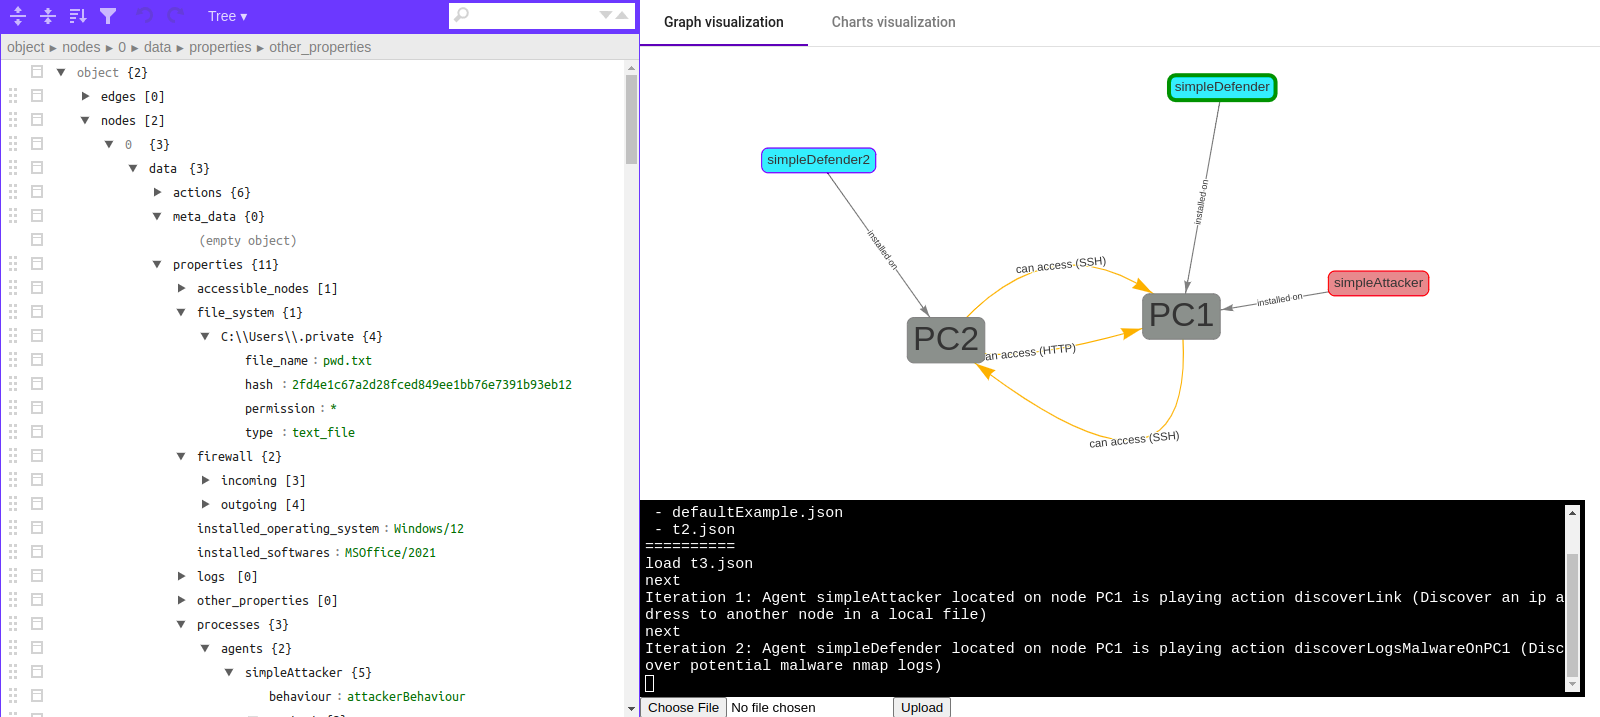
\includegraphics[width=\linewidth]{figures/interface_MCAS.png}
%      \caption{Simulator interface overview}
%      \label{fig:simulator_interface}
% \end{figure}

The development of our model has led to the \textquote{Multi Cyber Agent Simulator} (MCAS)~\cite{MCASWebsite} simulator. In the current state of development, this simulator allows loading/saving a \textit{json} file describing the nodes properties and actions of the environment and the defined agents with their behaviors; and launching the execution of the agents of this environment in turn-by-turn mode via the terminal. It is possible to view the environment properties in real time and visualize the environment in the form of a graph. Metrics are displayed as well.



\subsection{MITRE ATT\&CK based case study}

% \rem{Expliquer pourquoi on veut tester les capacités du simulateur -> illustration de comment fonctionne le simulateur}
% \rem{Gallium APT, pourquoi ce choix ? pourquoi ce cas d'étude inspiré de ça ? Qu'est-ce qui est interessant dans Gallium APT ? Type d'attaque/ coordination d'attaque ?}

\noindent
Intending to assess coordinated attacks and collective defense, we chose GALLIUM APT (a cyberespionage group active since 2012), for it allows defining several concurrent attacks.


\subsubsection{Network topology}

% \rem{Pour chaque élément présent dans la figure, faire le lien avec les éléments cités dans la présentation de la topologie...}

\noindent
Based on some GALLIUM APT tactics we selected some associated techniques/sub-techniques to propose a small company like networked environment, presented in Figure~\ref{fig:scenario_network_topology}. It is divided in 5 subnets communicating through implicit routers positioned after a firewall:
The outside subnet used to represent external attackers as if in the same network for convenience. It includes two desktop computers (At1 and At2).
The Demilitarized Zone (DMZ) subnet is used to separate devices that are accessible from the Internet from the rest of the company's network. The servers in the DMZ include a web server (WS), an email server (ES), a VPN server (VPN), and a FTP server (FTP), all connected bidirectionally both to outside and inside the company network.
The first local area network (ACC) subnet used to connect devices within the accounting department of the company where employee are working in. It contains two employee workstations (E1 and E2) and a Chief Technical Officer workstation (CTO), all connected bidirectionally to the DMZ. % and only accessible from SRV (defined below);
The second local area network (MAR) subnet used to connect devices within the marketing department of the company. It contains a printer server (PS), one employee workstations (E3) and tablet terminal (TAB) connected via a wireless access point, all connected bidirectionally to the DMZ. %and only accessible from SRV (defined below);
The third local area network (SRV) subnet used to connect the company devices providing services. It contains an API server (API), a database server (DB), and a domain controller (DC).

\begin{figure}
    \centering
    \includesvg[width=\linewidth]{figures/topology.svg}
    \caption{Proposed small-scale company network topology}
    \label{fig:scenario_network_topology}
\end{figure}


%These devices are accessible from the DMZ and from the CTO. API is also accessible via a VPN tunnel from the outside.

% The simulated machines are populated with files, folders, firewall rules, network services, and so on, so both attackers and defenders can have more actions to interact.


\subsubsection{Scenario and agent implementation with evaluation}

\begin{figure}
    \centering
    \includesvg[width=\linewidth]{figures/graphs.svg}
    \caption{An evolution of the rewards average according to episodes in small-scale tests with MARL and Decision Tree Approaches with inactive cyber-defense
    }
    \label{fig:graphs}
\end{figure}

\noindent
The cyber-attacker agents are initially deployed on At1 and At2 and the cyber-defender agents are deployed on WS and DB. The ultimate attackers' goals is to get data from the DB server and installing one spyware on the printer server PS. Following our approach in ~\ref{sec:ad_integration} we propose an AD tree presented in Figure~\ref{fig:ADTree}. It only shows the paths of the attacks to follow to reach the ultimate goal while the defender actions can prevent these at several stages of the attack.
We first interested in setting up the two cyber-attackers behaviors, then the two cyber-defenders' ones. We simulated an abstracted version of the scenario over 1000 episodes.

% In addition, we implemented some other common actions to interact with the file system, OS configuration, firewall configuration, and network services. These actions can be derived from the attack/defense actions but are implicitly not shown in the AD tree. Yet, they are taken into account in the simulation so agents can explore action paths even if this does not lead to an ultimate attacker goal.


%\subsubsection{Scenario execution and evaluation}

\noindent
\textbf{Random approach}: \quad The random agent only choose its actions by exploring the whole action space without any criteria until reaching the goal. In our case study, the shortest action path for attackers to reach the ultimate goal contains 16 different actions among the 30 defined actions, hence a low probability of $(1/30)^{16}$.
This approach allows getting a benchmark of unexpected edge failure cases and to compare with other types of agent.

\noindent
\textbf{Decision Tree (DT) approach}: \quad The decision tree was applied to get a reference when cyber-attackers or cyber-defenders already know the best action to take as the role of each agent is defined by a DT.
In Figure~\ref{fig:graphs}, the $DT\_attacker1$ follows an action path to reach the goal of installing a custom spyware in PS. In the same time, $DT\_attacker2$ reaches the goal of exfiltrating data in DB and completing the action path by getting the flag. Then we added the defenders $DT\_defender1$ which has to detect malicious logs on WS and $DT\_defender2$ which has to use privilege account management or monitor the executed commands and arguments on DB. We observed the attackers to be unable to reach the ultimate goal.

\noindent
\textbf{Multi-Agent Reinforcement Learning (MARL) approach}: \quad Q-Learning~\cite{CWatkins1992} was applied with curriculum learning for first the attackers learn how to reach the ultimate attack goal before adding defenders.
In the Figure~\ref{fig:graphs}, $MARL\_attacker1$ and $MARL\_attacker2$ follow a same behavior ultimately refining the applied actions to the relevant ones to reach the ultimate goal. After several episodes, chosen action paths by the attackers tend to be as efficient as the DT paths. When adding the defenders $MARL\_defender1$ and $MARL\_defender2$, we verified the attackers to be less and less able to reach the ultimate goal.


\subsection{Conclusion and perspectives}

\noindent
We proposed a Dec-POMDP modeling of networked node likely to be attacked and defended by agents. This model aims to integrate scenarios. The implementation of this model led to a simulator whose some capabilities have been assessed through a MITRE ATT\&CK scenario. Using three approaches, we briefly checked how decision tree, random and reinforcement learning approaches can be applied to agent for comparison.
Willing to take advantage of this simulation approach to address realistic issues related to cyber-defenders, particularly in the AICA context, we identified the main limitations to overcome:
automating the integration of more realistic scenarios leveraging on a basis of common actions and properties so agents can explore and act as in seemingly similar to reality information systems;
establishing a way to use the benefits of results obtained with simulations for emulated or real systems while maintaining agent behaviors during deployment;
having more coordination between agents, such as several entry points or scenarios with needed communication to reach a goal\dots;
and introducing new constraints in actions (such as cost, execution duration, etc.).

\section{Un scénario d'essaim de drones}

\textit{Autonomous Intelligent Cyberdefense Agents}~\cite{Kott2023} (AICA) are agents to be deployed in networked environments to detect, identify, and characterize anomalies/attacks, develop countermeasures, and execute them
%
\footnote{
    Theorized by the \textit{AICA International Work Group} (cf. \url{https://www.aica-iwg.org/}) and based on the results of NATO's \textit{Research Task Group IST-152}.
}.
Related AICA research highlights the increasing need for \textit{Autonomous Cyberdefense} to protect decentralized environments where traditional centralized approaches are ineffective, such as in IoT-based systems. A Multi-Agent System (MAS) offers robust and adaptive defense mechanisms by decomposing the complexity of Cyberdefense into sub-tasks delegated to collaborative agents deployed throughout the system.

The top-down approach involves designing Cyberdefense MAS from predefined architectures and functionalities. The \textit{MAS Centric AICA Reference Architecture} (MASCARA)~\cite{Kott2023} describes an AICA-like MAS with components that enable collaborative mechanisms based on explicitly defined plans or processes. However, this approach can be costly as it requires comprehensive knowledge of the deployment environment, which must be regularly updated due to frequent changes, such as topology modifications or new vulnerabilities.

The bottom-up approach may include Multi-Agent Reinforcement Learning (MARL)~\cite{Albrecht2024}, where agents learn to achieve Cyberdefense goals autonomously, enhancing MAS autonomy~\cite{hammar_stadle4_noms_23}. Despite promising simulation results, this approach lacks the safety guarantees necessary for real-world applications and does not provide explicit means to justify the MAS's success or failure~\cite{dulacarnold2019}. These issues hinder the development of fully or semi-autonomous Cyberdefense MAS, such as AICA, in critical environments, where actions must be justified given their potentially irreversible consequences.

To address this concern, we propose combining these two points of view by extending the \textit{Partial Relation between Agents' History and Organizational Model}~\cite{soule2024} (PRAHOM). PRAHOM is a general approach that enables integrating the $\mathcal{M}OISE^+$ organizational model into the MARL framework, laying the foundation for constraining learning. However, this perspective remains limited in its implementation and faces scalability issues with the number of organizational specifications, which limits its application in complex networked environments.

The main contribution of this paper is the \textit{Cyberdefense-oriented PRAHOM} (CoPRAHOM) inspired by PRAHOM and related works. This algorithm is specifically intended to address Cyberdefense scenarios relying on general Cyberdefense architectures such as MASCARA. This algorithm enables users to constrain agents to Cyberdefense roles and missions. We implemented practical means to apply CoPRAHOM also aiming to address scalability concerns. One of the main interests is to ensure safety guarantees by embedding domain-specific knowledge, such as rules, or accelerating or stabilizing the training by restricting the search space.

We assessed CoPRAHOM in the simulated scenario provided by the 3rd CAGE Challenge~\cite{cage_challenge_3_announcement}. It involves creating a Cyberdefense MAS for detecting, mitigating, and eliminating malware programs in a drone swarm. Using CoPRAHOM, we developed several Cyberdefense MAS models. These models are used by CoPRAHOM to guide and constrain agents' training to better achieve the scenario's goals and ensure safety requirements. We verify that the trained agents exhibit expected collective strategies while being also fine-tuned throughout the training, making the overall score comparable to leading entries on the leaderboard.


\subsection{MARL Background}\label{sec:marl_background}

Multi-Agent Reinforcement Learning (MARL) extends the principles of Reinforcement Learning (RL) to scenarios involving multiple interacting agents. Agents aim to maximize the overall cumulative reward through learning, but the presence of other agents introduces additional complexity due to the dynamic nature of the environment.

MARL is often modeled using the Decentralized Partially Observable Markov Decision Process (Dec-POMDP)~\cite{Beynier2013}, a framework suitable for environments where agents have limited and differing observations. A Dec-POMDP is formally defined as a tuple $(S, \{A_i\}, T, R, \{\Omega_i\}, O, \gamma)$:

\begin{itemize}
    \item $S$: A finite set of states describing the environment.
    \item $\{A_i\}$: A set of action sets, one for each agent $i$.
    \item $T$: The state transition probability function $T(s, \vec{a}, s') = P(s'|s, \vec{a})$, where $\vec{a}$ is the joint action of all agents.
    \item $R$: The reward function $R(s, \vec{a}, s')$, mapping states and actions to a reward.
    \item $\{\Omega_i\}$: A set of observation sets, one for each agent $i$.
    \item $O$: The observation probability function $O(\vec{o} | s', \vec{a})$, where $\vec{o}$ is the joint observation of all agents.
    \item $\gamma \in [0,1]$: The discount factor for future rewards.
\end{itemize}

In MARL, each agent $i$ maintains a policy $\pi_i: H \times \Omega \rightarrow A$, mapping an action $a \in A$ from an observation $\omega \in \Omega$ and optionally the agent's history $h \in H, h=\langle(\omega_0,a_0),(\omega_1,a_1)\dots(\omega_{n_e},a_{n_e})\rangle$ (with $n_e \in \mathbb{N}$, the number of steps per episode). A joint policy $\pi_{\text{joint}} = (\pi_1, \pi_2, \ldots, \pi_n)$ describes the behavior of all agents collectively.

The ultimate goal is to find a joint policy $\pi_{\text{joint}}$ that maximizes the expected cumulative reward $U(\pi^*_{\text{joint}}) = \mathbb{E}\left[\sum_{t=0}^{\infty} \gamma^t R(s_t, \vec{a}_t)\right]$. Instead of solely aiming for a global optimum, our approach emphasizes obtaining approximate solutions with sufficient reward.

Various methods have been proposed to address the challenges of MARL.
%
\textbf{Value-based methods}, such as QMIX~\cite{rashid2018}, estimate the value function $Q(s,\vec{a})$, which represents the expected cumulative reward for a given state $s$ and joint action $\vec{a}$. While these methods have shown promising results in simple scenarios, they often struggle to effectively utilize multi-agent communication to enhance overall rewards~\cite{oroojlooy2021review}.
%
\textbf{Policy-based methods}, including Multi-Agent Proximal Policy Optimization (MAPPO)\cite{yu2022surprising} and Multi-Agent Deep Deterministic Policy Gradient (MADDPG)\cite{lowe2017multi}, directly parameterize the policy as $\pi_\theta$ and optimize it, potentially using centralized training with decentralized execution. We have preferred these methods because they have demonstrated significant efficiency in various cooperative and competitive multi-agent contexts~\cite{yu2022surprising}\cite{lowe2017multi}.
%
Lastly, \textbf{Actor-Critic methods} combine value-based and policy-based approaches. For instance, in COMA (Counterfactual Multi-Agent Policy Gradients), the actor updates the policy parameters in the direction indicated by the critic, which evaluates the current policy. Although these methods have proven efficient in single-agent settings, additional efforts are needed to fully adapt them to multi-agent scenarios, particularly in managing the complexity introduced by agents' mutual influence~\cite{papoudakis2021agent}.


\subsection{Related Works}
\label{sec:related_works}

We define organizational-oriented MARL as the broad field of research encompassing studies that introduce explicit specifications (such as rules, roles, or protocols) to guide or restrict the MARL training process to meet requirements. While the explicit integration of organizational specifications in MARL is not extensively covered in the literature, several approaches have been proposed to embed some constraints within MAS to ensure that agents conform to specific requirements.

\textbf{Learning with Organizational Constraints} \quad
In \cite{cruz2020norms}, the authors present a method for incorporating norms into the learning algorithms of agents, ensuring that their behavior remains within acceptable bounds. Additionally, \cite{villatoro2011social} proposes a mechanism for agents to learn and adapt to social norms in dynamic environments, highlighting the importance of norm adaptation in MAS.
%
A relevant subset of work belongs to \emph{Specification-Guided Reinforcement Learning}, which aims to generate policies that accomplish specific tasks using external specifications to guide learning in achieving objectives under given constraints~\cite{Bansal2022}. Jothimurugan et al.~\cite{Jothimurugan2021} propose logical specification learning, exploiting the compositional structure of specifications to generate policies for complex tasks. However, it does not completely fall into the MARL framework we set for it requires introducing logical specifications.

\textbf{MARL in Cybersecurity and Autonomous Cyber Operations} \quad
MARL has also been applied in cybersecurity to develop autonomous systems capable of defending against cyber threats. Albrecht et al.~\cite{Albrecht2024} explore the use of MARL for training agents in dynamic environments to achieve cybersecurity goals.
As previously stated in Kott et al.~\cite{Kott2023}, some works involved by AICAs include the development of simulation frameworks for hand-tailored training of autonomous agents in a decentralized environment~\cite{Drasar2020}.
Similarly, in \cite{Hammar2022}, the authors present a framework using \emph{system identification} methods for integrating digital twins with MARL to enhance cybersecurity automation and enhance MARL applicability in real systems.

\textbf{Policy-Based Approaches} \quad
Some works related to policy-based approaches foster ways to enforce organizational constraints by defining explicit policies that govern agent behavior. In \cite{krupanski2015norm}, the use of normative policies is investigated to guide agent interactions and decision-making processes. Moreover, \cite{vos2020governing} explores the use of governance mechanisms to enforce compliance with organizational policies in decentralized systems. However, these approaches face a lack of practicality in their use and may be difficult to explain since most policies are black-box and cannot be easily modified.

\textbf{Frameworks Integrating Organizational Aspects} \quad
Wang et al.~\cite{Wang2020} introduce an approach in which similar emerging roles are encouraged to jointly specialize in specific tasks. Tosic et al.~\cite{Tosic2010} propose a framework for coordination based on the communication capabilities of multi-agent systems. Zheng et al.~\cite{Zheng2018} present a platform for MARL that aims to facilitate research on artificial collective intelligence by providing a comprehensive set of evaluation metrics to compare the performance of MARL algorithms. However, it does not take into account specifications likely to entice agents to adhere to an expected behavior such as missions.


Despite these advancements, there is still a scarcity of research explicitly utilizing organizational specifications to constrain agent learning in accordance with requirements. To our knowledge, no existing work facilitates the generation of a MAS that explicitly satisfies additional organizational constraints. CoPRAHOM's originality lies in using an organizational model explicitly as a general way for constraining learning based on these requirements.

\subsection{Combining $\mathcal{M}OISE^+$ Model with MARL}
\label{sec:marl_moise_linking}

This section briefly presents the principles we propose for adapting MARL with organizational specifications to align policies with expected role behaviors and mission goals.

The $\mathcal{M}OISE^+$ model provides a structured framework for defining roles and interactions within a Multi-Agent System (MAS). It is compatible with MARL, allowing for formal descriptions of agent policies. The CoPRAHOM approach embeds $\mathcal{M}OISE^+$ specifications into MARL training, enabling agents to adhere to predefined roles and missions. $\mathcal{M}OISE^+$ defines \textbf{Organizational Specifications (OS)} as $\mathcal{OS} = \langle \mathcal{SS}, \mathcal{FS}, \mathcal{DS} \rangle$, where $\mathcal{SS}$ are \textbf{Structural Specifications}, $\mathcal{FS}$ are \textbf{Functional Specifications}, and $\mathcal{DS}$ are \textbf{Deontic Specifications}.

\subsubsection{Structural Specifications}

\textbf{Structural Specifications} ($\mathcal{SS} = \langle \mathcal{R}, \mathcal{IR}, \mathcal{G} \rangle$) describe organizational structure:
\begin{itemize}
    \item $\mathcal{R}_{ss}$: All roles ($\rho \in \mathcal{R}$).
    \item $\mathcal{IR}$: Role inheritance relation ($\rho_1 \sqsubset \rho_2$).
    \item $\mathcal{RG} \subseteq \mathcal{GR}$: Root groups, $\mathcal{GR} = \langle \mathcal{R}, \mathcal{SG}, \mathcal{L}^{intra}, \mathcal{L}^{inter}, \mathcal{C}^{intra}, \mathcal{C}^{inter}, np, ng \rangle$, where:
          \begin{itemize}
              \item $\mathcal{R}$: Non-abstract roles.
              \item $\mathcal{SG}$: Sub-groups.
              \item $\mathcal{L}^{intra}$ and $\mathcal{L}^{inter}$: Intra and inter group links denoted as a 3-tuple $(\rho_s, \rho_d, t)$, where $t \in \{acq, com, aut\}$.
              \item $\mathcal{C}^{intra}$ and $\mathcal{C}^{inter}$: Intra and inter group compatibilities denoted as $\rho_a \bowtie \rho_b$.
              \item $np$: Cardinality of agents in a role.
              \item $ng$: Cardinality of each sub-group.
          \end{itemize}
\end{itemize}

Direct policy constraints are impractical due to black-box models like neural networks. Instead, we represent roles as history subsets $\mathcal{P}(H)$ that agents should generate, characterizing expected behaviors. Each role maps to a history subset via $rh: \mathcal{R} \rightarrow \mathcal{P}(H)$. Agents' policies should generate histories belonging to these subsets.

We address large, complex observations by using labels to represent observations. The mapping $ol: \mathcal{P}(\Omega) \rightarrow \mathcal{P}(L)$ translates observations to labels, potentially using a trained Large Language Model (LLM). This simplifies defining history subsets, which can be represented by patterns, rules, or custom scripts.

\begin{figure}[h!]
    \centering
    


\tikzset{every picture/.style={line width=0.75pt}} %set default line width to 0.75pt        

\begin{tikzpicture}[x=0.75pt,y=0.75pt,yscale=-1,xscale=1]
%uncomment if require: \path (0,1800); %set diagram left start at 0, and has height of 1800

%Shape: Rectangle [id:dp9341453924522656] 
\draw  [fill={rgb, 255:red, 255; green, 255; blue, 255 }  ,fill opacity=1 ] (160,44) -- (510,44) -- (510,167) -- (160,167) -- cycle ;
%Shape: Rectangle [id:dp4628140741854456] 
\draw  [fill={rgb, 255:red, 184; green, 233; blue, 134 }  ,fill opacity=0.34 ] (374,52) -- (504,52) -- (504,162) -- (374,162) -- cycle ;
%Shape: Rectangle [id:dp6461749357206974] 
\draw  [fill={rgb, 255:red, 184; green, 233; blue, 134 }  ,fill opacity=0.34 ] (378,78) -- (500,78) -- (500,158) -- (378,158) -- cycle ;
%Shape: Rectangle [id:dp47018118728898073] 
\draw  [fill={rgb, 255:red, 248; green, 231; blue, 28 }  ,fill opacity=0.4 ] (164,48) -- (314,48) -- (314,162) -- (164,162) -- cycle ;
%Straight Lines [id:da37904402438854] 
\draw    (400,150.31) -- (400,193.69) ;
\draw [shift={(400,195.69)}, rotate = 270] [color={rgb, 255:red, 0; green, 0; blue, 0 }  ][line width=0.75]    (10.93,-3.29) .. controls (6.95,-1.4) and (3.31,-0.3) .. (0,0) .. controls (3.31,0.3) and (6.95,1.4) .. (10.93,3.29)   ;
\draw [shift={(400,148.31)}, rotate = 90] [color={rgb, 255:red, 0; green, 0; blue, 0 }  ][line width=0.75]    (10.93,-3.29) .. controls (6.95,-1.4) and (3.31,-0.3) .. (0,0) .. controls (3.31,0.3) and (6.95,1.4) .. (10.93,3.29)   ;
%Straight Lines [id:da30557994145553513] 
\draw    (368,140) -- (386,140) ;
\draw [shift={(388,140)}, rotate = 180] [color={rgb, 255:red, 0; green, 0; blue, 0 }  ][line width=0.75]    (10.93,-3.29) .. controls (6.95,-1.4) and (3.31,-0.3) .. (0,0) .. controls (3.31,0.3) and (6.95,1.4) .. (10.93,3.29)   ;
%Shape: Rectangle [id:dp15689957472567295] 
\draw  [fill={rgb, 255:red, 248; green, 231; blue, 28 }  ,fill opacity=0.4 ] (169.56,76) -- (309.06,76) -- (309.06,157) -- (169.56,157) -- cycle ;
%Shape: Rectangle [id:dp6202366628126772] 
\draw  [fill={rgb, 255:red, 255; green, 255; blue, 255 }  ,fill opacity=1 ] (372,196) -- (414,196) -- (414,216) -- (372,216) -- cycle ;

%Shape: Rectangle [id:dp20067598884831228] 
\draw  [fill={rgb, 255:red, 248; green, 231; blue, 28 }  ,fill opacity=0.4 ] (212.06,129) -- (234.06,129) -- (234.06,149) -- (212.06,149) -- cycle ;

%Shape: Rectangle [id:dp5970765798398485] 
\draw  [fill={rgb, 255:red, 248; green, 231; blue, 28 }  ,fill opacity=0.4 ] (178.06,129) -- (203.06,129) -- (203.06,149) -- (178.06,149) -- cycle ;
%Shape: Rectangle [id:dp92237875722883] 
\draw  [fill={rgb, 255:red, 248; green, 231; blue, 28 }  ,fill opacity=0.4 ] (178.06,102) -- (218.06,102) -- (218.06,122) -- (178.06,122) -- cycle ;

%Shape: Rectangle [id:dp6591761395302378] 
\draw  [fill={rgb, 255:red, 248; green, 231; blue, 28 }  ,fill opacity=0.4 ] (178.06,80) -- (218.06,80) -- (218.06,100) -- (178.06,100) -- cycle ;

%Shape: Rectangle [id:dp11794703752595392] 
\draw  [fill={rgb, 255:red, 248; green, 231; blue, 28 }  ,fill opacity=0.4 ] (258.5,80) -- (298.5,80) -- (298.5,100) -- (258.5,100) -- cycle ;

%Shape: Rectangle [id:dp6557958558103134] 
\draw  [fill={rgb, 255:red, 248; green, 231; blue, 28 }  ,fill opacity=0.4 ] (259,102) -- (299,102) -- (299,122) -- (259,122) -- cycle ;

%Shape: Rectangle [id:dp8284992701408749] 
\draw  [fill={rgb, 255:red, 65; green, 117; blue, 5 }  ,fill opacity=1 ] (388,129) -- (410,129) -- (410,149) -- (388,149) -- cycle ;

%Shape: Rectangle [id:dp7066110016250453] 
\draw  [fill={rgb, 255:red, 248; green, 231; blue, 28 }  ,fill opacity=0.4 ] (244,129) -- (266,129) -- (266,149) -- (244,149) -- cycle ;

%Shape: Rectangle [id:dp4021333114319714] 
\draw  [fill={rgb, 255:red, 248; green, 231; blue, 28 }  ,fill opacity=0.4 ] (170.31,53) -- (195.69,53) -- (195.69,73) -- (170.31,73) -- cycle ;

%Shape: Rectangle [id:dp8476756388266236] 
\draw  [fill={rgb, 255:red, 248; green, 231; blue, 28 }  ,fill opacity=0.4 ] (200,53) -- (226,53) -- (226,73) -- (200,73) -- cycle ;

%Shape: Rectangle [id:dp07470576340681823] 
\draw  [fill={rgb, 255:red, 74; green, 144; blue, 226 }  ,fill opacity=1 ] (324,101) -- (364,101) -- (364,121) -- (324,121) -- cycle ;

%Shape: Rectangle [id:dp31407652093057714] 
\draw  [fill={rgb, 255:red, 74; green, 144; blue, 226 }  ,fill opacity=1 ] (324,129) -- (364,129) -- (364,149) -- (324,149) -- cycle ;

%Shape: Rectangle [id:dp053729126169398844] 
\draw  [fill={rgb, 255:red, 184; green, 233; blue, 134 }  ,fill opacity=0.34 ] (378,55) -- (404,55) -- (404,75) -- (378,75) -- cycle ;

%Shape: Rectangle [id:dp7720103442630182] 
\draw  [fill={rgb, 255:red, 184; green, 233; blue, 134 }  ,fill opacity=0.34 ] (405.94,103) -- (431.94,103) -- (431.94,123) -- (405.94,123) -- cycle ;

%Shape: Rectangle [id:dp3183552657000306] 
\draw  [fill={rgb, 255:red, 184; green, 233; blue, 134 }  ,fill opacity=0.34 ] (447.44,103) -- (473.44,103) -- (473.44,123) -- (447.44,123) -- cycle ;

%Shape: Rectangle [id:dp10802424702469593] 
\draw  [fill={rgb, 255:red, 184; green, 233; blue, 134 }  ,fill opacity=0.34 ] (466,129) -- (488,129) -- (488,149) -- (466,149) -- cycle ;

%Shape: Rectangle [id:dp16589412198505937] 
\draw  [fill={rgb, 255:red, 184; green, 233; blue, 134 }  ,fill opacity=0.34 ] (428,129) -- (450,129) -- (450,149) -- (428,149) -- cycle ;

%Shape: Rectangle [id:dp1270989692188249] 
\draw  [fill={rgb, 255:red, 255; green, 255; blue, 255 }  ,fill opacity=1 ] (258,196) -- (300,196) -- (300,216) -- (258,216) -- cycle ;

%Straight Lines [id:da40017392935840324] 
\draw    (286,149.69) -- (286,193.69) ;
\draw [shift={(286,195.69)}, rotate = 270] [color={rgb, 255:red, 0; green, 0; blue, 0 }  ][line width=0.75]    (10.93,-3.29) .. controls (6.95,-1.4) and (3.31,-0.3) .. (0,0) .. controls (3.31,0.3) and (6.95,1.4) .. (10.93,3.29)   ;
\draw [shift={(286,147.69)}, rotate = 90] [color={rgb, 255:red, 0; green, 0; blue, 0 }  ][line width=0.75]    (10.93,-3.29) .. controls (6.95,-1.4) and (3.31,-0.3) .. (0,0) .. controls (3.31,0.3) and (6.95,1.4) .. (10.93,3.29)   ;
%Shape: Rectangle [id:dp21027747628033966] 
\draw  [fill={rgb, 255:red, 245; green, 166; blue, 35 }  ,fill opacity=1 ] (276,129) -- (298,129) -- (298,149) -- (276,149) -- cycle ;

%Shape: Rectangle [id:dp5582162899072272] 
\draw  [fill={rgb, 255:red, 255; green, 255; blue, 255 }  ,fill opacity=1 ] (172,178) -- (184,178) -- (184,190) -- (172,190) -- cycle ;
%Straight Lines [id:da3472969066473863] 
\draw    (170,210) -- (192,210) ;
\draw [shift={(194,210)}, rotate = 180] [color={rgb, 255:red, 0; green, 0; blue, 0 }  ][line width=0.75]    (6.56,-1.97) .. controls (4.17,-0.84) and (1.99,-0.18) .. (0,0) .. controls (1.99,0.18) and (4.17,0.84) .. (6.56,1.97)   ;
\draw [shift={(168,210)}, rotate = 0] [color={rgb, 255:red, 0; green, 0; blue, 0 }  ][line width=0.75]    (6.56,-1.97) .. controls (4.17,-0.84) and (1.99,-0.18) .. (0,0) .. controls (1.99,0.18) and (4.17,0.84) .. (6.56,1.97)   ;
%Shape: Rectangle [id:dp07012270906311535] 
\draw  [fill={rgb, 255:red, 255; green, 255; blue, 255 }  ,fill opacity=1 ] (332,197) -- (354,197) -- (354,217) -- (332,217) -- cycle ;

%Straight Lines [id:da7534392810513293] 
\draw    (344,164) -- (344,194) ;
\draw [shift={(344,196)}, rotate = 270] [color={rgb, 255:red, 0; green, 0; blue, 0 }  ][line width=0.75]    (10.93,-3.29) .. controls (6.95,-1.4) and (3.31,-0.3) .. (0,0) .. controls (3.31,0.3) and (6.95,1.4) .. (10.93,3.29)   ;
\draw [shift={(344,162)}, rotate = 90] [color={rgb, 255:red, 0; green, 0; blue, 0 }  ][line width=0.75]    (10.93,-3.29) .. controls (6.95,-1.4) and (3.31,-0.3) .. (0,0) .. controls (3.31,0.3) and (6.95,1.4) .. (10.93,3.29)   ;
%Straight Lines [id:da4125176624573814] 
\draw    (320,140) -- (300,140) ;
\draw [shift={(298,140)}, rotate = 360] [color={rgb, 255:red, 0; green, 0; blue, 0 }  ][line width=0.75]    (10.93,-3.29) .. controls (6.95,-1.4) and (3.31,-0.3) .. (0,0) .. controls (3.31,0.3) and (6.95,1.4) .. (10.93,3.29)   ;
%Shape: Rectangle [id:dp005426842763594397] 
\draw  [fill={rgb, 255:red, 80; green, 227; blue, 194 }  ,fill opacity=0.36 ] (320,76) -- (368,76) -- (368,162) -- (320,162) -- cycle ;
%Straight Lines [id:da9128713017721406] 
\draw    (478,150.31) -- (478,193.69) ;
\draw [shift={(478,195.69)}, rotate = 270] [color={rgb, 255:red, 0; green, 0; blue, 0 }  ][line width=0.75]    (10.93,-3.29) .. controls (6.95,-1.4) and (3.31,-0.3) .. (0,0) .. controls (3.31,0.3) and (6.95,1.4) .. (10.93,3.29)   ;
\draw [shift={(478,148.31)}, rotate = 90] [color={rgb, 255:red, 0; green, 0; blue, 0 }  ][line width=0.75]    (10.93,-3.29) .. controls (6.95,-1.4) and (3.31,-0.3) .. (0,0) .. controls (3.31,0.3) and (6.95,1.4) .. (10.93,3.29)   ;
%Shape: Rectangle [id:dp7604827971406838] 
\draw  [fill={rgb, 255:red, 255; green, 255; blue, 255 }  ,fill opacity=1 ] (450,196) -- (492,196) -- (492,216) -- (450,216) -- cycle ;



% Text Node
\draw (465,179) node   [align=left] {$gh$};
% Text Node
\draw (181.5,204) node  [font=\tiny] [align=left] {$name$};
% Text Node
\draw (334,179) node   [align=left] {$da$};
% Text Node
\draw (222,207) node  [font=\footnotesize] [align=left] {\begin{minipage}[lt]{29.67pt}\setlength\topsep{0pt}
\begin{center}
{\small Relation}
\end{center}

\end{minipage}};
% Text Node
\draw (202,185) node  [font=\footnotesize] [align=left] {\begin{minipage}[lt]{13.75pt}\setlength\topsep{0pt}
\begin{center}
{\small Set}
\end{center}

\end{minipage}};
% Text Node
\draw (343.5,61) node   [align=left] {$\mathcal{OS}$};
% Text Node
\draw (190.56,139) node   [align=left] {$\mathcal{SG}$};
% Text Node
\draw (345,85) node   [align=left] {$\mathcal{DS}$};
% Text Node
\draw (245.5,61) node   [align=left] {$\mathcal{SS}$};
% Text Node
\draw (387,179) node   [align=left] {$mh$};
% Text Node
\draw (275.5,177) node   [align=left] {$rh$};
% Text Node
\draw (237.56,91) node   [align=left] {$\mathcal{G}r$};
% Text Node
\draw (440.5,65) node   [align=left] {$\mathcal{FS}$};
% Text Node
\draw (439.44,90) node   [align=left] {$\mathcal{SCH}$};
% Text Node
\draw (472,205) node   [align=left] {$\mathcal{P}(H)$};
% Text Node
\draw (343,207) node   [align=left] {$\mathcal{A}$};
% Text Node
\draw (287,139) node   [align=left] {$\mathcal{R}$};
% Text Node
\draw (280,205) node   [align=left] {$\mathcal{P}(H)$};
% Text Node
\draw (439,139) node   [align=left] {$\mathcal{P}$};
% Text Node
\draw (477,139) node   [align=left] {$\mathcal{G}$};
% Text Node
\draw (460.44,113) node   [align=left] {$nm$};
% Text Node
\draw (418.94,113) node   [align=left] {$mo$};
% Text Node
\draw (391,65) node   [align=left] {$\mathcal{PO}$};
% Text Node
\draw (345,139) node   [align=left] {$\mathcal{OBL}$};
% Text Node
\draw (345,111) node   [align=left] {$\mathcal{PER}$};
% Text Node
\draw (214,62) node   [align=left] {$\mathcal{R}_{ss}$};
% Text Node
\draw (183,63) node   [align=left] {$\mathcal{IR}$};
% Text Node
\draw (255,139) node   [align=left] {$\mathnormal{ng}$};
% Text Node
\draw (399,139) node   [align=left] {$\mathcal{M}$};
% Text Node
\draw (280,112) node   [align=left] {$\mathcal{C}^{inter}$};
% Text Node
\draw (279.5,90) node   [align=left] {$\mathcal{C}^{intra}$};
% Text Node
\draw (199.06,90) node   [align=left] {$\mathcal{L}^{intra}$};
% Text Node
\draw (199.06,112) node   [align=left] {$\mathcal{L}^{inter}$};
% Text Node
\draw (223.06,139) node   [align=left] {$np$};
% Text Node
\draw (394,205) node   [align=left] {$\mathcal{P}(H)$};


\end{tikzpicture}
    \caption{Relations between organizational specifications and history subsets}
    \label{fig:PRAHOM_osm_rels}
\end{figure}

A history subset constrains a policy to a role. We introduce \textbf{observable policy constraints} $c\pi: H \times \Omega \rightarrow \mathcal{P}(A)$, dictating allowable actions per observation. These constraints integrate into policies in three modes:
\begin{itemize}
    \item \textbf{Correct}: Adjusts any chosen action $\pi(\omega)$ to an expected one in $c\pi(\omega)$, ensuring safety.
    \item \textbf{Penalize}: Adds a penalty for actions $\pi(\omega) \notin c\pi(\omega)$, encouraging agents to learn constraints.
    \item \textbf{Correct\_Policy}: Creates a \textbf{constrained policy} $\pi_c$ where $c\pi$ corrects $\pi$, ensuring internal safety.
\end{itemize}

\subsubsection{Functional Specifications}

\textbf{Functional Specifications} ($\mathcal{FS} = \langle \mathcal{SCH}, \mathcal{PO} \rangle$) define tasks and goals:
\begin{itemize}
    \item $\mathcal{SCH} = \langle \mathcal{G}, \mathcal{M}, \mathcal{P}, mo, nm \rangle$: Social schemes, where:
          \begin{itemize}
              \item $\mathcal{G}$: Global goals.
              \item $\mathcal{M}$: Mission labels.
              \item $\mathcal{P}$: Plans $(g_f, \{g_i\}_{0 \leq i \leq s}, op, ps)$.
              \item $mo$: Goals for each mission.
              \item $nm$: Cardinality of agents per mission.
          \end{itemize}
    \item $\mathcal{PO}$: Preference orders $(m_1 \prec m_2)$.
\end{itemize}

Goals are represented as history subsets, $gh: \mathcal{G} \rightarrow \mathcal{P}(H)$. Missions map to expected histories $mh: \mathcal{M} \rightarrow \mathcal{P}(H)$. Goals impact MARL by updating the reward function, enticing agents to generate desired histories. We introduce \textbf{observable reward functions} $R_g: H \rightarrow \mathbb{R}$, measuring the closeness of generated histories to expected ones. Mission rewards are weighted sums of goal rewards, promoting faster convergence.

\subsubsection{Deontic Specifications}

\textbf{Deontic Specifications} ($\mathcal{DS} = \langle \mathcal{OBL}, \mathcal{PER} \rangle$) define permissions and obligations:
\begin{itemize}
    \item $\mathcal{TC}$: Time constraints.
    \item $\mathcal{OBL}$: Obligations $(obl(\rho_a, m, tc))$.
    \item $\mathcal{PER}$: Permissions $(per(\rho_a, m, tc))$.
\end{itemize}

The relation $da: \mathcal{PER} \cup \mathcal{OBL} \rightarrow \mathcal{P}(\mathcal{A})$ constrains roles and missions with time limits, managed by $dttl: \mathcal{PER} \cup \mathcal{OBL} \times \mathcal{A} \rightarrow \mathbb{N}$. Obligations have higher reward multipliers than permissions, prioritizing mission adherence.

These principles integrate organizational specifications into the MARL framework, forming the CoPRAHOM algorithm.

\subsection{A Cyberdefense-oriented MARL Algorithm}\label{sec:coprahom}

In this section, we shortly recap the MASCARA architecture as a general abstract Cyberdefense organizational $\mathcal{M}OISE^+$ model to be used jointly with CoPRAHOM.
Then, we detail the CoPRAHOM algorithm as well as its practical implementation for concrete Cyberdefense scenarios.
%we introduce CoPRAHOM, a novel algorithm that integrates the MASCARA architecture with the principles of $\mathcal{M}OISE^+$ to address Cyberdefense challenges in Multi-Agent Reinforcement Learning (MARL). This integration facilitates the training of agents that adhere to predefined organizational roles and missions in the context of Cyberdefense.

\subsubsection{A General Cyberdefense Architecture as a foundation}

The MASCARA architecture is designed for AICAs. It includes components such as a Decision-Making Engine, Knowledge Base, Online Learning Engine, Agent Behavior Engine, Orchestrator, Workspace, Collaboration Interface, and Internal Communication Protocol. These components work together to monitor, detect, and respond to cyber threats.
%
% Converting the MASCARA architecture into the $\mathcal{M}OISE^+$ model is advantageous for addressing various Cyberdefense challenges because:

% \begin{itemize}
%     \item \textbf{Structured Representation}: $\mathcal{M}OISE^+$ provides a structured representation of roles, interactions, and goals, which aligns well with the hierarchical and functional nature of MASCARA.
%     \item \textbf{Role and Mission Specification}: $\mathcal{M}OISE^+$ allows for precise specification of roles and missions, ensuring that each agent's behavior is aligned with the overall Cyberdefense strategy.
%     \item \textbf{Deontic Relations}: The deontic specification in $\mathcal{M}OISE^+$ helps in defining permissions and obligations for agents, which is crucial in a dynamic and reactive Cyberdefense environment.
% \end{itemize}

The abstract general Cyberdefense organizational model derived from MASCARA can be represented using $\mathcal{M}OISE^+$. The most important ones include:
%
% \begin{itemize}
%     \item \textbf{Structural Specifications} ($\mathcal{SS}$): Define roles such as \textit{Intrusion Detector}, \textit{Traffic Analyzer}, \textit{Response Coordinator}, and their relationships.
%     \item \textbf{Functional Specifications} ($\mathcal{FS}$): Define missions like \textit{Detect Intrusion}, \textit{Analyze Malicious Traffic}, and \textit{Mitigate Attack}, each with specific goals and plans.
%     \item \textbf{Deontic Specifications} ($\mathcal{DS}$): Define permissions and obligations for roles to commit to missions based on situational awareness and predefined rules.
% \end{itemize}
%
% Linking each role or mission to an expected history subset requires defining patterns, protocols, logic, and rules that agents must follow. Below, we outline a framework for linking roles to expected history subsets:
%
\textbf{Intrusion Detector} which involves monitoring network traffic continuously; generating alerts upon detecting anomalies; and employing statistical models and anomaly detection algorithms.
%
\textbf{Traffic Analyzer} which focuses on analyzing packet contents for malicious signatures; correlating data from multiple sources; and using deep packet inspection and signature matching techniques.
%
\textbf{Response Coordinator} which executes predefined response plans; coordinates with other agents for a synchronized response; and evaluates the impact of different response strategies.


Most relevant missions include:
%
\textbf{Detect Intrusion} which aims at identifying unauthorized access attempts; deploying honeypots to attract attackers; and updating detection rules based on emerging threats.
%
\textbf{Analyze Malicious Traffic} which aims at collecting and examining traffic data; using machine learning models to classify traffic; and correlating findings with known attack patterns.
%
\textbf{Mitigate Attack} which aims at deploying countermeasures against identified threats; isolating affected systems and rerouting traffic; and prioritizing measures that minimize service disruption.

This overview presents an abstract model termed \textit{MASCARA-$\mathcal{M}OISE^+$}, designed as a flexible framework for specifying customized roles, missions, and interactions across various scenarios. The core concept of CoPRAHOM leverages the capability to partially define roles or missions of the aforementioned model through their associated expected history subsets. This partial definition allows for adaptive fine-tuning as new or unexpected situations arise that were not originally covered. Consequently, this premise led to the CoPRAHOM algorithm for implementing mechanisms to guide and constrain agents, compelling them to adhere to these predefined roles and missions. This approach not only facilitates real-time monitoring of agent activities but also ensures that their behaviors remain aligned with requirements.


\subsubsection{CoPRAHOM for Cyberdefense Scenarios}

The CoPRAHOM algorithm first requires defining a concrete $\mathcal{M}OISE^+$ organizational model (from the \textit{MASCARA-$\mathcal{M}OISE^+$} model) and describing how each role or mission should be in terms of history subsets in MARL.
% Then, it enables systematically integrating organizational specifications into the learning process by enforcing constraints on joint policies based on predefined roles, missions, and permission/obligation relationships.
This integration ensures that agents' behaviors are not only optimized for performance but also adhere to organizational requirements.
%
In this section, we informally present a detailed, step-by-step description of the CoPRAHOM algorithm and discuss its implementation in the \textit{CoPRAHOM Wrapper}.\\

\textbf{Initialization and Input Parameters}:
First, CoPRAHOM initializes the joint policy with the initial joint policy, and sets the episode counter to zero. Also, sets a boolean variable called "sufficient" to False, indicating that the cumulative reward expectancy has not yet been met. It is initialized with the role-to-history $rh$, mission-to-history $mh$, and deontic specifications to agent $da$ that describe how agents should be impacted during learning by predefined roles and missions.

\textbf{Step 1: Determine Joint Observable Policy Constraints}:
Identify the joint observable policy constraints from the organizational specifications using $rh$ and $da$ relations.

\textbf{Step 2: Initialize Constrained Policy}:
If the mode of constraint integration is set to "correct policy," create and use a joint constrained policy based on the initial policy and the observable policy constraints.

\textbf{Step 3: Determine Observable Reward Functions}:
Establish the observable reward functions from the organizational specifications. Integrate these observable reward functions within the global reward function.

\textbf{Step 4: Main Training Loop}:
Run the main training loop for a maximum number of episodes or until the cumulative reward expectancy is met.

\textbf{Initialize Episode}:
At the beginning of each episode, reinitialize the environment, observation, and action histories. Reset the cumulative reward and penalty. Initialize time-to-live values for permissions/obligations, and set the initial observation and action by the environment.

\textbf{Step Through Episode}:
During each episode, perform the following steps for a maximum number of steps:

\begin{itemize}
    \item Update the joint policy using the MARL algorithm based on the current history and last rewards;
    \item Select the next action based on the current observation;
    \item Identify the expected actions from the observable policy constraints. If the selected action is not among the expected ones, correct or penalize it based on the mode of constraint integration;
    \item Update the current history and apply the action to the environment to get the next observation and reward, adding any incurred penalties;
    \item Decrease time-to-live values, and update the reward functions and policies if some organizational specifications have changed.
\end{itemize}

\textbf{Check for Sufficiency}:
After each episode, check whether the cumulative reward meets the expectancy and increment the episode counter.


% \quad \emph{Implementation}:
% The wrapper uses the proposed \textit{train\_under\_constraint()} function to manage these initializations, accepting input parameters and setting the episode counter and sufficiency condition. This functions takes at least two arguments: the \textit{ol\_mngr} and the \textit{os} objects:

% The \textit{ol\_mngr} singleton is part of the API. It uses the HuggingFace transformer model \textit{tiiuae/falcon-7b} to learn mappings between real observations and short-way labels in conjunction with a simple dictionary. It also provides an interactive process for users to label each observation during the labeling procedure, essential for accurately detecting and categorizing cyber threats in a dynamic environment. Its interest lies in its use within a \textit{history\_subset}. This class handles history subsets based on predefined patterns or rules via an implemented history graph when dealing with patterns. \textit{ol\_mngr} eases the creation of a pattern letting users utilize explicit labels to craft an expected behavior conveniently. Alternatively, custom functions can be used within a history\_subset, providing flexibility to adapt to various Cyberdefense scenarios.

% The \textit{osr} class represents a $\mathcal{M}OISE^+$ organizational model in a JSON-like representation and is the backbone of the \emph{CoPRAHOM Wrapper}. In this class, roles and goals are directly mapped to observable policy constraints \textit{opc} and observable reward functions \textit{orf} objects using patterns, rules, or custom functions. This class implements role-to-history (rh), goal-to-history (gh), and mission-to-history (mh) mappings. Permissions and obligations are also defined here, with each obligation or permission mapped to agents, thus implementing the deontic-specification-to-agents relation (da).

\

To implement CoPRAHOM, we favored the \emph{PettingZoo} library, which offers a widely used and standardized API for developing multi-agent environments and using MARL algorithms~\cite{Terry2021}. We integrated the MARLlib~\cite{hu2022marllib} library that offers a significant amount of implemented MARL algorithms such as MAPPO or MADDPG as well as fine-tuned models for a wide range of environments. This implementation results in the \textit{CoPRAHOM Wrapper}, which extends the PettingZoo API with additional CoPRAHOM-specific features.
%
The CoPRAHOM Wrapper provides an API with additional auxiliary classes to define organizational specifications and link them to their expected behavior in a Cyberdefense context. These two main classes are the \textit{ol\_mngr} and the \textit{osr} objects.

The singleton class \textit{ol\_mngr}, as a part of the API, uses the HuggingFace transformer model \textit{tiiuae/falcon-7b} to learn mappings in conjunction with a simple dictionary.
%It also provides an interactive process for users to label each observation during the labeling procedure, essential for accurately detecting and categorizing cyber threats in a dynamic environment.
The \textit{osr} class gathers all previously instantiated elements into a complete $\mathcal{M}OISE^+$ organizational model, which is JSON-representable. In this class, roles and goals are directly mapped to observable policy constraint \textit{opc} and observable reward function \textit{orf} objects using patterns, rules, or custom functions. This class implements role-to-history (rh), goal-to-history (gh), and mission-to-history (mh) mappings. Permissions and obligations are also defined here, with each obligation or permission mapped to agents, thus implementing the deontic allocation (da) relation.

Once the PettingZoo environment is wrapped with the CoPRAHOM Wrapper and all auxiliary classes have been instantiated to get an \textit{ol\_mngr} and \textit{os}, the wrapper's API provides the \textit{train\_under\_constraint()} function. This function enables executing the CoPRAHOM algorithm, taking \textit{ol\_mngr} and \textit{os} objects as arguments, in addition to other MARLlib parameters. Ultimately, it generates MARLlib policy objects and statistical data, ensuring that agents are trained to meet the stringent requirements of Cyberdefense operations.

\subsection{Experimental Setup}\label{sec:experimental_setup}

In order to meet the requirements of the 3rd CAGE Challenge, our experimental setup involves creating Cyberdefense MAS models using $\mathcal{M}OISE^+$ organizational specifications. We established models with varying levels of constraints, including different roles and missions. For inspiration, we referred to the MASCARA architecture while developing these models. After implementing CoPRAHOM, we demonstrated its use in integrating the defined models to constrain agents' learning. Finally, we evaluated the impact of these models both during training and after deployment.

\subsubsection{3rd CAGE Challenge}

As illustrated in \autoref{fig:cage_challenge},
The 3rd CAGE Challenge simulates a fictional border conflict where Florin uses autonomous drones for military communication. The CybORG simulator models a drone swarm forming an ad-hoc network, which must be defended against malware programs (red agents) planted by Guilder's spies. The objective is to create autonomous defense systems (blue agents) that detect, respond to, and mitigate attacks, ensuring continuous communication for Florin's troops (green agents).

\begin{figure}
    \centering
    \begin{tikzpicture}
    % Define the positions of the drones
    \coordinate (A) at (0,2);
    \coordinate (B) at (2,2);
    \coordinate (C) at (1,3);
    \coordinate (D) at (3,3);
    \coordinate (E) at (4,2);
    \coordinate (F) at (5,3);
    \coordinate (G) at (6,2);
    
    % Draw the drones with the drone image
    \foreach \pos in {A,B,C,D,E,F,G} {
        \node at (\pos) {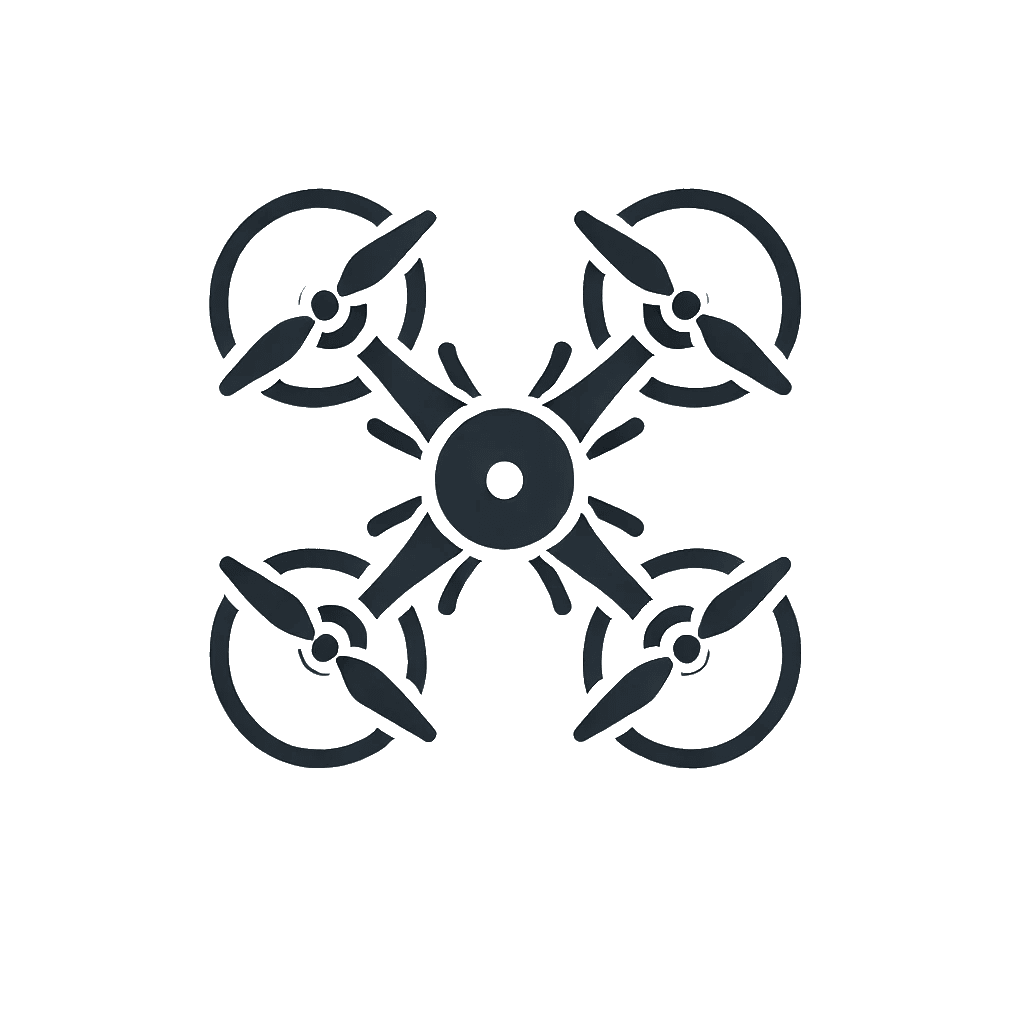
\includegraphics[width=1cm]{figures/drone_scheme.png}};
    }
    
    % Draw the connections
    \draw[dotted] (A) -- (B);
    \draw[dotted] (B) -- (C);
    % \draw[dotted] (B) -- (D);
    \draw[dotted] (D) -- (E);
    \draw[dotted] (E) -- (F);
    % \draw[dotted] (F) -- (G);
    
    % Add agent symbols as green circles
    \node[fill=green, circle, minimum size=7pt, inner sep=0pt] at (0.41,2.41) {};
    \node[fill=green, circle, minimum size=7pt, inner sep=0pt] at (2.41,2.41) {};
    \node[fill=green, circle, minimum size=7pt, inner sep=0pt] at (1.41,3.41) {};
    \node[fill=green, circle, minimum size=7pt, inner sep=0pt] at (3.41,3.41) {};
    \node[fill=green, circle, minimum size=7pt, inner sep=0pt] at (4.41,2.41) {};
    \node[fill=green, circle, minimum size=7pt, inner sep=0pt] at (5.41,3.41) {};
    \node[fill=green, circle, minimum size=7pt, inner sep=0pt] at (6.41,2.41) {};
    
    % Add blue circles to the left of some green circles
    \node[fill=blue, circle, minimum size=7pt, inner sep=0pt] at (0.11,2.41) {};
    \node[fill=blue, circle, minimum size=7pt, inner sep=0pt] at (2.11,2.41) {};
    \node[fill=blue, circle, minimum size=7pt, inner sep=0pt] at (3.11,3.41) {};
    \node[fill=blue, circle, minimum size=7pt, inner sep=0pt] at (5.11,3.41) {};
    
    % Add one additional circle to the left of an existing circle
    \node[fill=red, circle, minimum size=7pt, inner sep=0pt] at (4.11,2.41) {}; % Example: red circle added

    % Add the legend
    \node[fill=red, circle, minimum size=7pt, inner sep=0pt, label=right:{\small red agent}] at (0,1) {};
    \node[fill=blue, circle, minimum size=7pt, inner sep=0pt, label=right:{\small blue agent}] at (3,1) {};
    \node[fill=green, circle, minimum size=7pt, inner sep=0pt, label=right:{\small green agent}] at (6,1) {};
    
    \node at (1,0.5) {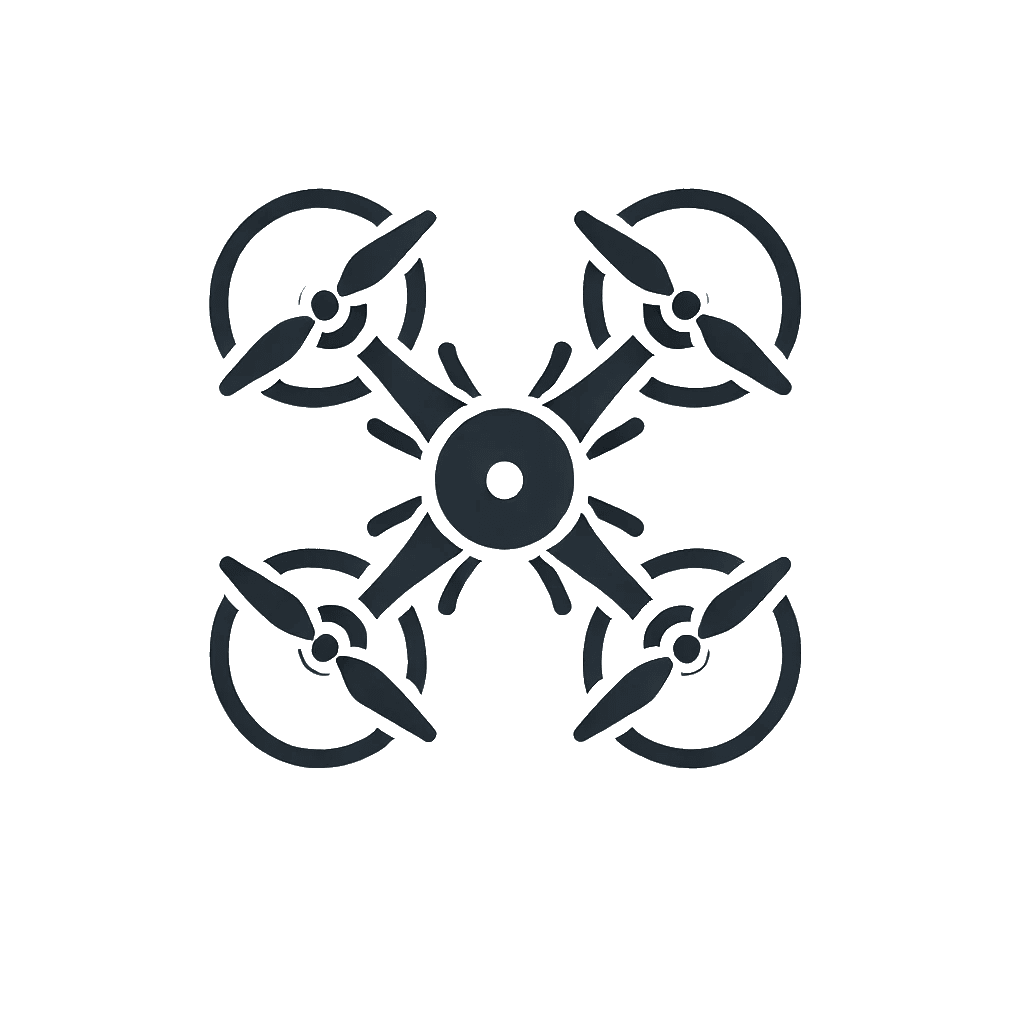
\includegraphics[width=1cm]{figures/drone_scheme.png}};
    \node[anchor=west] at (2,0.5) {\small drone};

    % Communication lines in legend
    \begin{scope}
        \draw[dotted] (4,0.5) -- (5,0.5);
        \node[anchor=west] at (5.1,0.5) {\small communication};
    \end{scope}
    
\end{tikzpicture}
    \caption{An illustrative view of the 3rd CAGE Challenge Scenario}\label{fig:cage_challenge}
\end{figure}

The scenario features three types of agents:
\begin{itemize}
    \item \textbf{Blue Agents (Defenders)}: Tasked with maintaining the security and functionality of the drone network. Their roles include controlling drones, preventing unauthorized access, and ensuring data integrity. They can perform actions such as \textit{RetakeControl}, \textit{RemoveOtherSessions}, and \textit{BlockTraffic}.
    \item \textbf{Red Agents (Attackers)}: Aim to compromise the drones to disrupt communication and control. They exploit vulnerabilities and can perform actions like \textit{ExploitDroneVulnerability}, \textit{SeizeControl}, and \textit{FloodBandwidth}.
    \item \textbf{Green Agents (Data Transfer)}: Simulate legitimate data communication to test the network's integrity, primarily through the \textit{SendData} action.
\end{itemize}

Each agent has a partial view of the environment, focusing on aspects such as network state, drone status, and communication observations. The reward structure for Blue agents is based on successful data transfers, control over drones, network security, and bandwidth management. Positive rewards are given for maintaining secure and functional communication, while penalties are imposed for losses in control, security breaches, and inefficient bandwidth usage.

This challenge emphasizes the need for advanced cybersecurity measures, efficient resource management, and effective multi-agent coordination, making it a relevant testbed for CoPRAHOM development.

\subsubsection{Organizational Models}

\begin{figure*}[h!]
    \centering
    


\tikzset{every picture/.style={line width=0.75pt}} %set default line width to 0.75pt        

\begin{tikzpicture}[x=0.75pt,y=0.75pt,yscale=-1,xscale=1]
%uncomment if require: \path (0,1662); %set diagram left start at 0, and has height of 1662

%Rounded Rect [id:dp17386115134623514] 
\draw  [fill={rgb, 255:red, 245; green, 166; blue, 35 }  ,fill opacity=1 ] (424.61,402.58) .. controls (424.61,397.69) and (428.57,393.73) .. (433.46,393.73) -- (633.15,393.73) .. controls (638.04,393.73) and (642,397.69) .. (642,402.58) -- (642,429.15) .. controls (642,434.04) and (638.04,438) .. (633.15,438) -- (433.46,438) .. controls (428.57,438) and (424.61,434.04) .. (424.61,429.15) -- cycle ;
%Straight Lines [id:da8877910798706699] 
\draw    (547.33,451.83) -- (547.33,440) ;
\draw [shift={(547.33,438)}, rotate = 90] [color={rgb, 255:red, 0; green, 0; blue, 0 }  ][line width=0.75]    (10.93,-3.29) .. controls (6.95,-1.4) and (3.31,-0.3) .. (0,0) .. controls (3.31,0.3) and (6.95,1.4) .. (10.93,3.29)   ;
%Shape: Rectangle [id:dp44726237549140535] 
\draw   (376,452.18) -- (654,452.18) -- (654,488.66) -- (376,488.66) -- cycle ;
%Shape: Rectangle [id:dp2820683536345354] 
\draw   (402,290.27) -- (664,290.27) -- (664,379.64) -- (402,379.64) -- cycle ;
%Right Arrow [id:dp4162270206865013] 
\draw   (330,436.09) -- (417,436.09) -- (417,434.78) -- (425.91,437.39) -- (417,440) -- (417,438.7) -- (330,438.7) -- cycle ;
%Straight Lines [id:da8267677953106705] 
\draw    (548,393.83) -- (548,382) ;
\draw [shift={(548,380)}, rotate = 90] [color={rgb, 255:red, 0; green, 0; blue, 0 }  ][line width=0.75]    (10.93,-3.29) .. controls (6.95,-1.4) and (3.31,-0.3) .. (0,0) .. controls (3.31,0.3) and (6.95,1.4) .. (10.93,3.29)   ;
%Straight Lines [id:da6319519397458309] 
\draw    (218,456) -- (218,414) ;
\draw [shift={(218,412)}, rotate = 90] [color={rgb, 255:red, 0; green, 0; blue, 0 }  ][line width=0.75]    (10.93,-3.29) .. controls (6.95,-1.4) and (3.31,-0.3) .. (0,0) .. controls (3.31,0.3) and (6.95,1.4) .. (10.93,3.29)   ;
\draw [shift={(218,458)}, rotate = 270] [color={rgb, 255:red, 0; green, 0; blue, 0 }  ][line width=0.75]    (10.93,-3.29) .. controls (6.95,-1.4) and (3.31,-0.3) .. (0,0) .. controls (3.31,0.3) and (6.95,1.4) .. (10.93,3.29)   ;


% Text Node
\draw (68.5,471.5) node  [font=\footnotesize] [align=left] {\begin{minipage}[lt]{35.92pt}\setlength\topsep{0pt}
\begin{center}
{\small Labels ($\displaystyle L$)}
\end{center}

\end{minipage}};
% Text Node
\draw (372.5,426.5) node  [font=\small] [align=left] {\textit{\textbf{Fine-tuning}}};
% Text Node
\draw  [fill={rgb, 255:red, 74; green, 144; blue, 226 }  ,fill opacity=1 ]  (411,311) -- (652,311) -- (652,374) -- (411,374) -- cycle  ;
\draw (531.5,342.5) node  [font=\scriptsize] [align=left] {... "security\_measures":\\\{"firewall\_status": "enabled",\\"antivirus\_status": "enabled",\\"quarantine\_status": "trojan.exploit quarantined"\}\}\}};
% Text Node
\draw  [fill={rgb, 255:red, 80; green, 227; blue, 194 }  ,fill opacity=1 ]  (532,461.66) -- (623,461.66) -- (623,480.66) -- (532,480.66) -- cycle  ;
\draw (577.5,471.16) node  [font=\scriptsize] [align=left] {Quarantine Active};
% Text Node
\draw (536,302.25) node  [font=\footnotesize] [align=left] {{\small "The associated observations are"}};
% Text Node
\draw (671,417) node  [font=\small] [align=left] {\begin{minipage}[lt]{36.9pt}\setlength\topsep{0pt}
\begin{center}
\textit{\textbf{Regular}}\\\textit{\textbf{use}}
\end{center}

\end{minipage}};
% Text Node
\draw (512,471.16) node  [font=\footnotesize] [align=left] {{\small "What are the observation of \ \ \ \ \ \ \ \ \ \ \ \ \ \ \ \ \ \ \ \ \ \ \ \ \ ?"}};
% Text Node
\draw (46,356.32) node  [font=\footnotesize] [align=left] {\begin{minipage}[lt]{59.79pt}\setlength\topsep{0pt}
\begin{center}
{\small Observations ($\displaystyle \Omega $)}
\end{center}

\end{minipage}};
% Text Node
\draw (164,440.5) node  [font=\small] [align=left] {\textit{\textbf{Labeling}}};
% Text Node
\draw (267.5,433) node  [font=\footnotesize] [align=left] {{\footnotesize "$\displaystyle \Omega $ to be associated}\\{\footnotesize with labels $\displaystyle L$..."}};
% Text Node
\draw (533.3,415.86) node  [font=\footnotesize] [align=left] {\begin{minipage}[lt]{99.33pt}\setlength\topsep{0pt}
\begin{center}
tiiuae/falcon-7b (chat LLM)
\end{center}

\end{minipage}};
% Text Node
\draw  [fill={rgb, 255:red, 80; green, 227; blue, 194 }  ,fill opacity=1 ]  (100,456) -- (352,456) -- (352,489) -- (100,489) -- cycle  ;
\draw (226,472.5) node  [font=\scriptsize] [align=left] {\mbox{-} Malware Detected \ \ \ \ \ \ \ \ \ \ \ \ \ \ - \ Quarantine Active\\\mbox{-} Unusual Network Activity \ \ \ - Blocked Suspicious IP};
% Text Node
\draw  [fill={rgb, 255:red, 74; green, 144; blue, 226 }  ,fill opacity=1 ]  (94,290) -- (390,290) -- (390,412) -- (94,412) -- cycle  ;
\draw (242,351) node  [font=\scriptsize] [align=left] {\{"timestamp": "2024-07-29T11:30:00Z", "drone\_id": "drone\_4",\\ \ "observations": \{ "anomalous\_behavior\_detected": true,\\ \ \ \ "malware\_alert": \{ "detected\_malware": "trojan.exploit",\\ \ \ \ \ \ "detection\_time": "2024-07-29T11:28:00Z",\\ \ \ \ \ \ "detection\_method": "signature\_based"\}...\\ \ \ \ "security\_measures": \{\\ \ \ \ \ \ "firewall\_status": "enabled", "antivirus\_status": "enabled",\\ \ \ \ \ \ "quarantine\_status": "trojan.exploit quarantined"\}\}\}};


\end{tikzpicture}
    \caption{LLM training and use for applying CoPRAHOM to the 3rd CAGE Challenge}\label{fig:llm_process}
\end{figure*}


We implemented and evaluated two organizational models using the \textit{MASCARA-$\mathcal{M}OISE^+$} model and tailored for the CybORG 3rd CAGE Challenge environment:

The "\textbf{Active Defense}" model implements proactive measures for threat anticipation, detection, and mitigation. It focuses on maintaining network security and functionality through predefined three roles:
%
\textit{Threat Assessor}: Monitors the network, identifying potential threats using advanced analytics;
\textit{Response Strategist}: Oversees response strategies to neutralize identified threats;
\textit{Network Guardian}: Ensures network integrity and availability by implementing security measures.
%
This model also includes the \textit{Proactive Threat Detection} mission which contains goals for early detecting of threats using predictive analytics.

The "\textbf{Suspect Isolation}" emphasizes identifying and isolating compromised network elements to contain threats through three roles:
%
\textit{Anomaly Detector}: Identifies anomalies indicating potential breaches;
\textit{Isolation Specialist}: Isolates compromised systems to prevent threat spread;
\textit{Incident Responder}: Coordinates response and executes isolation protocols.
%
This model also includes the \textit{Compromised Drone Detection} mission which contains goals for detecting compromised drones and isolating them from the network as well as the \textit{Containment and Isolation} mission which contains goals for isolating compromised systems from the network.

Additionally, we established a non MASCARA-based model called "\textbf{Manual}" based on our empirical understanding of the environment, serving as a baseline model.
We also considered a totally non-constrained case as "\textbf{Free}" to serve as a regular MARL reference for comparison.


\subsubsection{Experimental Procedure}

We trained each organizational model using the \textit{CoPRAHOM Wrapper} with the provided \textit{CybORG} simulator. The wrapper integrates organizational specifications and constraints during learning, enabling agents to learn and adapt their behavior based on predefined roles and missions.

We selected the MAPPO algorithm for its proven efficiency in cooperative multi-agent environments without the need for domain-specific algorithmic modifications or architectures~\cite{Yu2022}. We used the MAPPO-implemented algorithm model provided by MARLlib. Specifically, we configured the MAPPO model with a two-layer MLP network, comprising 128 neurons in the first layer and 256 in the second, optimized using Adam with a learning rate of 0.0003. These configurations were chosen based on preliminary experiments and available MARLlib fine-tuned hyper-parameters models. We launched the training over 70 iterations (each consisting of 128 episodes) in a Centralized Learning and Decentralized Execution manner.\\

To train the LLM with \texttt{ol\_mngr}, we explored the environment manually, step-by-step, using controlled policies. This approach allowed the agent to encounter the most relevant situations for detecting and mitigating malware programs. For example, these include situations where an agent receives messages we think to be suspicious or situations where an agent receives a confirmation to kill a process. Throughout this exploration, we collected, displayed (as JSON or graph representation), interpreted, and labeled several observations to a few keywords. This labeling helps in easily identifying collective behaviors based on visual observations, enabling better control of agents' actions. The whole training and use process is summarized in \autoref{fig:llm_process}

\subsubsection{Evaluation metrics}

We used various metrics to measure the impact of CoPRAHOM during and after training:
\begin{itemize}
    \item \textbf{Scalability}: Assesses the ability to manage a growing number of agents and obstacles based on computational resource usage.
    \item \textbf{Convergence Time}: The number of episodes required for the algorithm to reach a stable solution. Shorter convergence times indicate faster learning.
    \item \textbf{Standard Deviation}: Indicates the variability in the rewards obtained by the agents. A lower standard deviation signifies more consistent performance and potentially more stable organization.
    \item \textbf{Average Reward}: The mean reward obtained per episode reflects the overall performance of the algorithm.
    \item \textbf{Constraint Respect}: Assesses how well the agents adhere to the given organizational constraints. %It is calculated as the inverse of the number of times the constraints are not satisfied. High constraint respect means that the agents are effectively following the rules.
\end{itemize}

We also included these two Cyberdefense-specific metrics:
\begin{itemize}
    \item \textbf{Average Percentage of Infected Drones by Malware}: Measures the proportion of drones infected by malware during the simulation.
    \item \textbf{Average Percentage of Successful Malware Attacks}: Indicates the success rate of attacks on the drone swarm.
\end{itemize}

\subsubsection{Criteria for validation}

Using the aforementioned metrics, we defined criteria to assess the enhancement in Cyberdefense provided by CoPRAHOM compared to regular MARL learning, particularly focusing on the "Active Defense" model. The criteria are:

\begin{itemize}
    \item $\mathbf{C_1}$: We expect to manually notice some collective strategies, such as isolating suspicious activities or coordinating defensive maneuvers.
    \item $\mathbf{C_2}$: We expect to see faster convergence in the "Active Defense" or "Suspect Isolation" models than in the "Free" case, and "Manual" one to show a constant learning curve.
    \item $\mathbf{C_3}$: We expect higher rewards in the "Active Defense" or "Suspect Isolation" models compared to the "Free" case.
    \item $\mathbf{C_{4}}$: We expect the standard deviation to decrease from "Free" to "Active Defense" or "Suspect Isolation" models and from "Active Defense" or "Suspect Isolation" models to the "Manual" model, since agents are increasingly more constrained in their behavior.
    \item $\mathbf{C_{5}}$: We expect the constraint respect to be fully covered in \textit{correct} and \textit{correct\_policy} modes but not in the \textit{penalize} mode.
    \item $\mathbf{C_{6}}$: We expect the scalability to be handled in all of the cases.
    \item $\mathbf{C_7}$: Lower average percentage of infected drones in "Active Defense" or "Suspect Isolation" models compared to the "Free" case.
    \item $\mathbf{C_8}$: Lower average percentage of successful malware attacks in "Active Defense" or "Suspect Isolation" models compared to the "Free" case.

\end{itemize}

\subsection{Results and Discussion}\label{sec:results_and_discussion}

\autoref{fig:learning_curves} illustrates the learning curves for the "Suspect Isolation", "Active Defensive", and "Manual" models, indicating their convergence rates over training episodes.
\autoref{tab:metrics_comparison} summarizes the convergence time during training as well as the average rewards, standard deviation, average infection drone, and average malware attack achieved models after training over a dozen episodes.

\begin{figure}[ht]
    \centering
    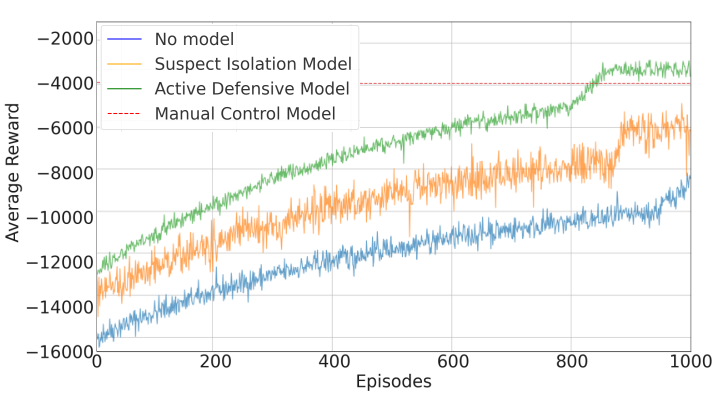
\includegraphics[width=1\linewidth]{figures/learning_curves.png}
    \caption{Learning curves for \textit{Free}, \textit{Suspect Isolation}, \textit{Active Defense}, \textit{Manual} using the \textit{correct\_policy} mode}
    \label{fig:learning_curves}
\end{figure}

\begin{table*}[t]
    \centering
    \setlength{\tabcolsep}{4.5pt}
    \caption{Comparison of models and constraint modes with respect to metrics.}
    \label{tab:metrics_comparison}
    \begin{tabular}{lcccccccccccc}
                               & {Free}      & \multicolumn{3}{c}{Suspect Isolation} & \multicolumn{3}{c}{Active Defense} & {Manual}                                                       \\
        % \cline{2-13}
        Metric                 &             & Penalize                              & Correct                              & Correct\_Policy  & Penalize & Correct  & Correct\_Policy &             \\
        \midrule
        Average Reward         & -8727.49    & -5900.00                              & -6085.12                             & -6088.00         & -3055.36 & -3100.00 & -3060.00        & -3906.00    \\
        Standard Deviation     & 138.00      & 2148.0                               & 2027.0                              & 2018.00          & 962.   & 940.00   & 945.00          & 570.33     \\
        Scalability            & Medium      & High                                  & Medium                               & Medium  & High     & Medium   & Medium & Medium      \\
        Convergence Time & >1000 & 1000 & 950 & 950 & 800 & 850 & 850 & $\emptyset$ \\
        Constraint Respect     & $\emptyset$ & Low                                   & High                                 & High             & Medium   & High     & High            & $\emptyset$      \\
        Avg. Inf. Drones (\%)  & 61.0        & 43.0                                  & 30.0                                 & 23.0             & 24.0     & 25.0     & 20.0            & 40.0        \\
        Avg. Malware Att. (\%) & 72.0        & 55.0                                  & 52.0                                 & 45.0             & 38.0     & 45.0     & 40.0            & 51.0        \\
    \end{tabular}
\end{table*}

The organizational models effectively influenced drone behavior in the CybORG CAGE Challenge 3 environment. The "Suspect Isolation" model demonstrated effective identification and isolation of drones exhibiting suspicious activities, enhancing overall security. This model ensured that potential threats were quickly identified and neutralized, preventing the spread of malicious activities within the drone swarm ($\mathbf{C_1}$).

\autoref{fig:learning_curves} provides a comprehensive view of the learning curves for each model. The "Free" model (blue) exhibited the slowest convergence and the lowest average rewards. Moreover, it also shows a low variability in rewards indicating that agents are slowly trained with limited changes at each step. This result is expected as the learning rate for MAPPO is relatively low.

In contrast, the "Suspect Isolation" model (orange) showed faster convergence and higher average rewards compared to the "Free" model. Yet, the increased variability (compared to "Free") suggests that since agents are forced/enticed to satisfy some rules to identify and isolate suspicious activities, their policies may require time to get used to these rules to reach a more stable behavior.

The "Active Defense" model (green) exhibited the highest average rewards and the fastest convergence among all models. The steadily increasing rewards demonstrate the efficiency of proactive defense strategies implemented by the agents. This model showed the greatest improvement in performance, underscoring the benefits of using structured organizational constraints to guide agent behavior. The "Active Defense" model also shows a lower variability in rewards compared to "Suspect Isolation" model but higher compared to the "Free" model. This suggests that while agents are still adapting to the constraints, their possible behaviors is more limited in "Active Defense" model than in "Suspect Isolation" model.

The "Manual" model (red dashed line) served as a baseline for comparison. It performed better than the "Free" and "Suspect Isolation" models but was outperformed by the "Active Defense" model. This can be explained as the manual control strategy, although effective, lacked the adaptability and efficiency provided by the learned organizational models.

From a quantitative perspective, the metrics also provide evidence for the advantages of applying organizational constraints. As illustrated in \autoref{fig:learning_curves}, in the constrained policy case, agents exhibited faster convergence compared to the "Free" model across all modes. This confirms that organizational constraints can accelerate learning ($\mathbf{C_2}$). The manually crafted policy case achieved immediate convergence, as expected, due to the absence of learning.

The average reward metrics reveal that agents guided by the "Suspect Isolation" model consistently outperformed those in the "Free" model, achieving higher rewards ($\mathbf{C_3}$). This indicates that organizational constraints not only improve learning efficiency but also enhance overall performance. The manually crafted policies consistently achieved the highest rewards, highlighting the efficiency of well-defined constraints.

Concerning constrained models, the standard deviation in \autoref{tab:metrics_comparison} decreased progressively from the less constrained model such as "Suspect Isolation" to the most constrained model such "Active Defense" ($\mathbf{C_4}$). This reduction in variability suggests that organizational constraints contribute to more stable and consistent agent behavior.

The criterion of constraint respect was fully met in the \textit{correct} and \textit{correct\_policy} modes, but not in the \textit{penalize} mode ($\mathbf{C_5}$). This demonstrates that while agents can learn to follow constraints effectively, the mode of constraint integration plays a crucial role. In our evaluation, the \textit{correct} and \textit{correct\_policy} modes demonstrated full adherence to organizational constraints, as evidenced by zero deviations in agent behavior from prescribed roles and missions. In contrast, the \textit{penalize} mode showed occasional deviations, particularly under high lesser constrained models such as "Suspect Isolation". This suggests that agents occasionally prioritize reward maximization over strict constraint adherence. Further analysis for penalization strategies would improve compliance.

Scalability, assessed by evaluating the system's performance under increased numbers of agents and obstacles, was effectively managed across all models ($\mathbf{C_6}$). Particularly, the \textit{penalize} mode showed superior scalability due to built-in efficient computation of policy updates, unlike the \textit{correct} and \textit{correct\_policy} modes that require aside correction functions.

Both "Active Defense" and "Suspect Isolation" models impacted the metrics for "Average Percentage of Infected Drones" and "Average Percentage of Successful Malware Attacks" ($\mathbf{C_7}$ and $\mathbf{C_8}$). Yet, it is important to note these two metrics are not directly related to the overall reward, since they are calculated separately. The "Active Defense" model achieved the best results, reducing the percentage of infected drones to 23\% and successful malware attacks to 38\%. This significant reduction, compared to the 61\% infection rate and 72\% success rate in the "Free" model, demonstrates the efficacy of proactive defensive strategies in preventing malware propagation and successful attacks. The "Suspect Isolation" model also showed lower infection and attack success rates than the "Free" model.

% These findings underscore the importance of implementing structured organizational constraints and proactive defense mechanisms within autonomous systems. The integration of $\mathcal{M}OISE^+$ organizational models within the MARL framework, as demonstrated by CoPRAHOM, proves to significantly enhance the efficiency and coordination of autonomous cyber defense agents. The experimental results highlight that structured organizational constraints not only improve agent performance and stability but also ensure that their behavior aligns with mission objectives and cybersecurity goals.

% The results suggest that further refinement of organizational specifications and incorporation of more sophisticated rules and protocols could yield even greater enhancements in agent behavior and coordination. This ongoing development promises to bolster the resilience and robustness of cyber defense strategies against increasingly sophisticated threats.
% However, CoPRAHOM's generalizability to different real-world Cyberdefense scenarios, such as IoT security or industrial control systems, may require adjustments in organizational specifications and policy constraints. Future work should explore these adaptations to validate CoPRAHOM's broad applicability.

\subsection{Conclusion}\label{sec:conclusion}

Our contribution is motivated by the high cost of designing Cyberdefense Multi-Agent Systems (MAS) in various scenarios, particularly when dealing with constantly evolving threats. To address this issue, we propose a dedicated algorithm called CoPRAHOM, that leverages Multi-Agent Reinforcement Learning (MARL) according to organizational specifications. CoPRAHOM ensures that some constraints are met in the agents' behavior, helping in the monitoring and understanding of the trained agents.

CoPRAHOM was evaluated using our proposed PoC implementation for the 3rd CAGE Challenge, a cooperative Cyberdefense drone swarm scenario designed to limit/eliminate malware programs and their impact. We established various organizational models, ranging from minimally constrained to fully constrained ones. We conducted an evaluation of the emergent, fine-tuned, or predefined collective strategies based on performance criteria during and after the training.

The results indicate that constraints-balanced models like the "Active Defensive Model" achieve a significant tradeoff between constraints and autonomous learning. This model employs straightforward predefined rules to detect and address threats when observations are unambiguous, while still allowing the agent to learn how to respond in other scenarios.

In addition to constraining agents according to organizational specifications, we aim to consider explainability mechanisms to understand newly learned organizational patterns. The idea of iterative improvement between training and explainability could greatly benefit from hierarchical learning, which helps characterize and bring out strategies during learning.
%Furthermore, while the initial results obtained with LLM show it as a promising complementary tool for CoPRAHOM, it may also offer new avenues for explaining collective behavior, especially in Cyberdefense scenarios where most networked environments are not visually or intuitively representable.

% Ultimately, we also aim to improve the applicability of PRAHOM by developing dedicated interfaces built around PRAHOM making it more accessible to industrial and research contexts.



\section{Un scénario d'Architecture de microservices}

% Contexte
Cloud-native critical systems are increasingly reliant on Kubernetes to orchestrate and manage interdependent services~\cite{Pahl2019}. HPA is a widely adopted mechanism to dynamically adjust the number of pods based on resource usage, enabling systems to handle highly dynamic workloads~\cite{Toka2020}. However, failures such as pod crashes, resource contention, and bottlenecks can severely jeopardize the performance of all of the cluster's functionalities we globally refer to as operational resilience~\cite{burns2016borg}. Worse, these failures may be exploited by attackers to degrade performance or induce outages, as seen in adversarial contexts like DDoS attacks~\cite{David2021}.

In such adversarial scenarios, malicious actors can exploit scaling mechanisms, exposing the limitations of conventional HPA systems. Modern approaches have sought to address these gaps using Reinforcement Learning (RL), where an agent optimizes a single global goal such as minimizing latency or resource usage~\cite{Gari2021}. While these methods demonstrate adaptability, they often fall short in handling diverse failure scenarios to maintain \textit{Quality of Service} (QoS)~\cite{Liu2024}. For example, prioritizing responses to cascading pod crashes during an attack may be far more critical than reducing latency. These challenges highlight the need for an autoscaling system capable of dynamically balancing multiple sub-goals to maintain all of the QoS to maximize operational resilience.

Achieving this shift from single-goal optimization to a multi-goal approach is complex~\cite{Shoham2009MAS}. A single-agent RL system struggles to address such complexity due to the difficulty of coordinating responses to diverse and context-dependent failures~\cite{Jennings1998}. In contrast, MASs offer a promising paradigm by decomposing the overarching operational resilience maximization goal into sub-goals handled by specialized agents~\cite{Shoham2009MAS}. Considering an adversarial scenario, each defender agent can collaboratively contribute to complementary scaling actions to reach its own sub-goal, enabling more resilient and context-specific responses face to an attacker agent~\cite{Jennings1998}. We refer to the set of these collaborative agents as an HPA MAS. An HPA MAS actually builds upon the cyberdefense framework of Autonomous Intelligent Cybersecurity Agents (AICAs), which can be viewed as agents with specialized roles and missions collaboratively defending systems against attackers~\cite{Kott2018}.

% Problématique
However, designing HPA MASs tailored to a cluster presents significant challenges such as the need for detailed cluster knowledge, the time-consuming nature of manual design processes, and the difficulty of ensuring optimal agent behavior. Moreover, cluster changes require repeating the design process, increasing operational costs and complexity.

% Contribution
Among methdological works, we inspired from the \textit{Assisted MAS Organization Engineering Approach} (AOMEA)~\cite{soule2024aomea} that shows to align the most with automation and safety challenges. Based on AOMEA, we propose the \textit{Kubernetes Autoscaling with Resilient Multi-Agent system} (KARMA) to automate the design and implementation process through four sequential activités:
\begin{enumerate}[label=\textbf{\arabic*)}, itemjoin={;\quad }]
    \item \textbf{Modeling}: Creating a digital twin of the cluster from real-world traces to simulate failure scenarios
    \item \textbf{Training}: Training agents in simulation using roles and missions that integrate explicit rule-based and guidance strategies
    \item \textbf{Analyzing}: Validating trained agents' behaviors and extracting design insights through empirical analysis
    \item \textbf{Transferring}: Running trained agents to apply their learned behaviors via the real Kubernetes API.
\end{enumerate}

This framework enables to iteratively updates the simulation model with newly collected traces, enabling adaptation to cluster changes. We validated our approach on adversarial scenarios from the "Chained Service" Kubernetes environment. The MASs were generated with minimal manual intervention and demonstrate originality. They compete with state-of-the-art HPA systems, including AWARE~\cite{aware2023}, Gym-HPA~\cite{gymhpa2022}, and Rlad-core~\cite{Rossi2019}, in maximizing operational resilience.

% Organisation
The remainder is structured as follows:
\autoref{sec:related_work} reviews existing HPA techniques and their limitations in dynamic environments.
\autoref{sec:proposed_approach} details our framework leveraging related concepts for each activité.
\autoref{sec:experiments} describes the experimental setup.
\autoref{sec:results} presents and discusses results.
\autoref{sec:conclusion} concludes and provides future directions.

% ===================================

\subsection{Related Work}
\label{sec:related_work}

\begin{table}[h!]
    \centering
    \caption{A KARMA overview regarding selected HPA Systems}
    \label{tab:autoscaling_criteria}
    {\footnotesize
    \renewcommand{\arraystretch}{1.1}
    % \resizebox{0.5\textwidth}{!}{%
    \begin{tabular}{>{\raggedright\arraybackslash}m{1.3cm}>{\centering\arraybackslash}m{0.6cm}>{\centering\arraybackslash}m{0.6cm}>{\centering\arraybackslash}m{0.6cm}>{\centering\arraybackslash}m{0.6cm}>{\centering\arraybackslash}m{0.6cm}>{\centering\arraybackslash}m{0.6cm}>{\centering\arraybackslash}m{0.6cm}>{\centering\arraybackslash}m{0.6cm}>{\centering\arraybackslash}m{0.6cm}}
    \hline
    \textbf{Criterion} & \vspace{-0.3cm}\textbf{\cite{gymhpa2022}} & \vspace{-0.3cm}\textbf{\cite{aware2023}} & \vspace{-0.3cm}\textbf{\cite{Rossi2019}} & \vspace{-0.3cm}\textbf{\cite{QoSRL}} & \vspace{-0.3cm}\textbf{\cite{Zhou2024}} & \vspace{-0.3cm}\textbf{\cite{KOSMOS}} & \vspace{-0.3cm}\textbf{\cite{COPA}} \\
    \hline
    \hline
    Adversarial Scenarios & No & Partial & No & No & No & No & Partial \\
    \hline
    Multi-goal & No & Yes & Partial & Yes & No & Yes & No \\
    \hline
    Automation & High & Mid. & Mid. & High & Mid. & Mid. & Mid. \\
    \hline
    Learning & Yes & Yes & Yes & Yes & No & No & No \\
    \hline
    MAS & No & No & No & No & No & No & No \\
    \hline
    Simulation & Yes & No & Yes & Yes & No & No & No \\
    \hline
    Real env. & No & Yes & Yes & Yes & Yes & Yes & Yes \\
    \hline
    Explainable & No & No & No & No & No & No & No \\
    \hline
    Adaptation & High & Mid. & Mid. & Mid. & High & High & Mid. \\
    \hline
    Safety Guarantees & No & No & No & No & No & No & No \\
    \hline
    \end{tabular}%
    }
  \end{table}


\noindent Autoscaling in Kubernetes has traditionally relied on metrics-based approaches, such as the default Kubernetes Horizontal Pod Autoscaler (KHPA), which adjusts the number of pods based on CPU and memory utilization~\cite{Carrion2022}. While effective for basic scaling, such methods fail to address dynamic or adversarial workloads, as they rely on reactive, threshold-based rules~\cite{Tran2022}. To overcome these limitations, recent research has turned to Machine Learning (ML) and RL.

% \subsection*{Reinforcement Learning-Based Systems}
Three RL-based systems stand out for their innovative approaches, applicability, and relevance:
%
\begin{itemize}
    \item \textbf{Gym-HPA}~\cite{gymhpa2022} serves as a benchmark RL environment, enabling experimentation with various RL algorithms. It excels in adaptability to simulated workloads with a high degree of automation but lacks multi-goal support, explainability, and real-world applicability
    \item \textbf{AWARE}~\cite{aware2023} incorporates RL to optimize autoscaling decisions while balancing QoS goals, such as response time and throughput. It partially considers adversarial scenarios but struggles with high automation levels and multi-agent coordination
    \item \textbf{Rlad-core}~\cite{Rossi2019} focus on both horizontal and vertical scaling introducing a self-adaptive system that dynamically adjusts resource allocation in response to workload variations, optimizing performance while minimizing costs.
\end{itemize}

These systems highlight significant progress in RL-based autoscaling but share common limitations: a lack of comprehensive adversarial adaptability, limited support for MAS, and no explicit focus on explainability or safety guarantees.
%
% \subsection*{Hybrid and Rule-Based Approaches}
Other notable systems combine ML or rule-based strategies with traditional autoscaling:
%
\begin{enumerate}[label={}, itemjoin={;\quad }]
    \item \textbf{QoS-Aware RL}~\cite{QoSRL} focus on maintaining QoS under dynamic workloads but does not integrate seamlessly with Kubernetes-native features or consider adversarial scenarios
    \item \textbf{AHPA}~\cite{Zhou2024} and \textbf{KOSMOS}~\cite{KOSMOS} explore adaptive and combined vertical-horizontal scaling strategies, offering high adaptability but lacking learning capabilities
    \item \textbf{COPA}~\cite{COPA} emphasize combined metrics-based autoscaling but remains reactive and limited in adversarial scenarios.
\end{enumerate}

% \subsection*{Positioning Our Contribution}
KARMA addresses key gaps in \textbf{(1) operational resilience} for autoscaling by introducing an automated HPA MAS design framework. Unlike conventional approaches, which often fail under \textbf{(2) adversarial conditions}, KARMA decomposes maintaining operational resilience into failure-specific missions and roles, enabling agents to handle coordinate response to \textbf{bottlenecks}, \textbf{resource contention}, \textbf{DDoS}, and \textbf{pod crashes}. It combines \textbf{(3) digital twin modeling} with \textbf{(4) automated MAS generation} via Multi-Agent Reinforcement Learning (MARL) integrating \textbf{constraint satisfaction} to these roles and missions, streamlining HPA MAS design with minimal manual intervention. Leveraging this decomposition, KARMA seeks for a better \textbf{(5) adaptability} while also enabling a better \textbf{(6) explainability} as for decision making in the whole HPA MAS.


% ===================================
\subsection{KARMA: A framework for HPA MAS design and development}
\label{sec:proposed_approach}

This section overviews the KARMA framework to helps in designing a HPA MAS then details each one of its activité.

\subsubsection{KARMA Overview}

\begin{figure}[h!]
    \centering
    


\tikzset{every picture/.style={line width=0.75pt}} %set default line width to 0.75pt        

\begin{tikzpicture}[x=0.75pt,y=0.75pt,yscale=-1.2,xscale=1.2]
%uncomment if require: \path (0,1414); %set diagram left start at 0, and has height of 1414

%Straight Lines [id:da5609883377896374] 
\draw [color={rgb, 255:red, 74; green, 144; blue, 226 }  ,draw opacity=1 ][line width=2.25]    (317.22,111.13) -- (360.07,111.13) ;
\draw [shift={(365.07,111.13)}, rotate = 180] [fill={rgb, 255:red, 74; green, 144; blue, 226 }  ,fill opacity=1 ][line width=0.08]  [draw opacity=0] (5.72,-2.75) -- (0,0) -- (5.72,2.75) -- cycle    ;
%Image [id:dp9396292457736715] 
\draw (106.77,60.95) node  {
\includegraphics[width=18.66pt,height=18.36pt]{figures/karma_architecture/pod.png}};
%Image [id:dp3874378335758297] 
\draw (145.86,60.95) node  {
\includegraphics[width=18.66pt,height=18.36pt]{figures/karma_architecture/pod.png}};
%Shape: Rectangle [id:dp4562827234223257] 
\draw  [color={rgb, 255:red, 74; green, 144; blue, 226 }  ,draw opacity=1 ][line width=1.5]  (89,28.36) .. controls (89,25.6) and (91.24,23.36) .. (94,23.36) -- (255,23.36) .. controls (257.76,23.36) and (260,25.6) .. (260,28.36) -- (260,132) .. controls (260,134.76) and (257.76,137) .. (255,137) -- (94,137) .. controls (91.24,137) and (89,134.76) .. (89,132) -- cycle ;
%Image [id:dp9455935833751838] 
\draw (172.5,16.24) node  {
\includegraphics[width=18.66pt,height=18.36pt]{figures/karma_architecture/kubernetes.png}};
%Shape: Rectangle [id:dp9564725691593288] 
\draw  [color={rgb, 255:red, 74; green, 144; blue, 226 }  ,draw opacity=1 ][line width=1.5]  (92.55,50.21) .. controls (92.55,47.45) and (94.79,45.21) .. (97.55,45.21) -- (155.08,45.21) .. controls (157.84,45.21) and (160.08,47.45) .. (160.08,50.21) -- (160.08,70.81) .. controls (160.08,73.57) and (157.84,75.81) .. (155.08,75.81) -- (97.55,75.81) .. controls (94.79,75.81) and (92.55,73.57) .. (92.55,70.81) -- cycle ;
%Image [id:dp9120856447688912] 
\draw (126.32,39.97) node  {
\includegraphics[width=18.66pt,height=18.36pt]{figures/karma_architecture/node.png}};
%Image [id:dp5738167237736518] 
\draw (106.77,119.52) node  {
\includegraphics[width=18.66pt,height=18.36pt]{figures/karma_architecture/pod.png}};
%Image [id:dp2199681121060142] 
\draw (145.86,119.52) node  {
\includegraphics[width=18.66pt,height=18.36pt]{figures/karma_architecture/pod.png}};
%Shape: Rectangle [id:dp12159705904547402] 
\draw  [color={rgb, 255:red, 74; green, 144; blue, 226 }  ,draw opacity=1 ][line width=1.5]  (92.55,108.78) .. controls (92.55,106.02) and (94.79,103.78) .. (97.55,103.78) -- (155.08,103.78) .. controls (157.84,103.78) and (160.08,106.02) .. (160.08,108.78) -- (160.08,129.38) .. controls (160.08,132.14) and (157.84,134.38) .. (155.08,134.38) -- (97.55,134.38) .. controls (94.79,134.38) and (92.55,132.14) .. (92.55,129.38) -- cycle ;
%Image [id:dp37768653229718074] 
\draw (126.32,98.54) node  {
\includegraphics[width=18.66pt,height=18.36pt]{figures/karma_architecture/node.png}};
%Shape: Rectangle [id:dp20840815212238661] 
\draw  [color={rgb, 255:red, 74; green, 144; blue, 226 }  ,draw opacity=1 ][line width=1.5]  (264,28.36) .. controls (264,25.6) and (266.24,23.36) .. (269,23.36) -- (411.78,23.36) .. controls (414.54,23.36) and (416.78,25.6) .. (416.78,28.36) -- (416.78,132) .. controls (416.78,134.76) and (414.54,137) .. (411.78,137) -- (269,137) .. controls (266.24,137) and (264,134.76) .. (264,132) -- cycle ;
%Straight Lines [id:da9232180983272227] 
\draw [color={rgb, 255:red, 74; green, 144; blue, 226 }  ,draw opacity=1 ][line width=2.25]    (164,112) -- (201,112) ;
\draw [shift={(206,112)}, rotate = 180] [fill={rgb, 255:red, 74; green, 144; blue, 226 }  ,fill opacity=1 ][line width=0.08]  [draw opacity=0] (5.72,-2.75) -- (0,0) -- (5.72,2.75) -- cycle    ;
%Straight Lines [id:da6082715106712999] 
\draw [color={rgb, 255:red, 74; green, 144; blue, 226 }  ,draw opacity=1 ][line width=2.25]    (180,90.22) -- (167,90.22) ;
\draw [shift={(162,90.22)}, rotate = 360] [fill={rgb, 255:red, 74; green, 144; blue, 226 }  ,fill opacity=1 ][line width=0.08]  [draw opacity=0] (5.72,-2.75) -- (0,0) -- (5.72,2.75) -- cycle    ;
%Straight Lines [id:da30764510910060716] 
\draw [color={rgb, 255:red, 74; green, 144; blue, 226 }  ,draw opacity=1 ][line width=2.25]    (210,72) -- (199,72) ;
\draw [shift={(194,72)}, rotate = 360] [fill={rgb, 255:red, 74; green, 144; blue, 226 }  ,fill opacity=1 ][line width=0.08]  [draw opacity=0] (5.72,-2.75) -- (0,0) -- (5.72,2.75) -- cycle    ;
%Straight Lines [id:da5394403186779959] 
\draw [color={rgb, 255:red, 74; green, 144; blue, 226 }  ,draw opacity=1 ][line width=2.25]    (178,56.22) -- (167,56.22) ;
\draw [shift={(162,56.22)}, rotate = 360] [fill={rgb, 255:red, 74; green, 144; blue, 226 }  ,fill opacity=1 ][line width=0.08]  [draw opacity=0] (5.72,-2.75) -- (0,0) -- (5.72,2.75) -- cycle    ;
%Straight Lines [id:da6399475815904785] 
\draw [color={rgb, 255:red, 74; green, 144; blue, 226 }  ,draw opacity=1 ][line width=2.25]    (272,72) -- (235,72) ;
\draw [shift={(230,72)}, rotate = 360] [fill={rgb, 255:red, 74; green, 144; blue, 226 }  ,fill opacity=1 ][line width=0.08]  [draw opacity=0] (5.72,-2.75) -- (0,0) -- (5.72,2.75) -- cycle    ;
%Straight Lines [id:da24320102833940327] 
\draw [color={rgb, 255:red, 74; green, 144; blue, 226 }  ,draw opacity=1 ][line width=2.25]    (267,112) -- (230,112) ;
\draw [shift={(272,112)}, rotate = 180] [fill={rgb, 255:red, 74; green, 144; blue, 226 }  ,fill opacity=1 ][line width=0.08]  [draw opacity=0] (5.72,-2.75) -- (0,0) -- (5.72,2.75) -- cycle    ;
%Shape: Rectangle [id:dp9149123987409296] 
\draw  [color={rgb, 255:red, 255; green, 255; blue, 255 }  ,draw opacity=1 ][fill={rgb, 255:red, 255; green, 255; blue, 255 }  ,fill opacity=1 ] (328.83,106.67) -- (353.11,106.67) -- (353.11,114) -- (328.83,114) -- cycle ;
%Image [id:dp7127891043436136] 
\draw (341.68,109.47) node  {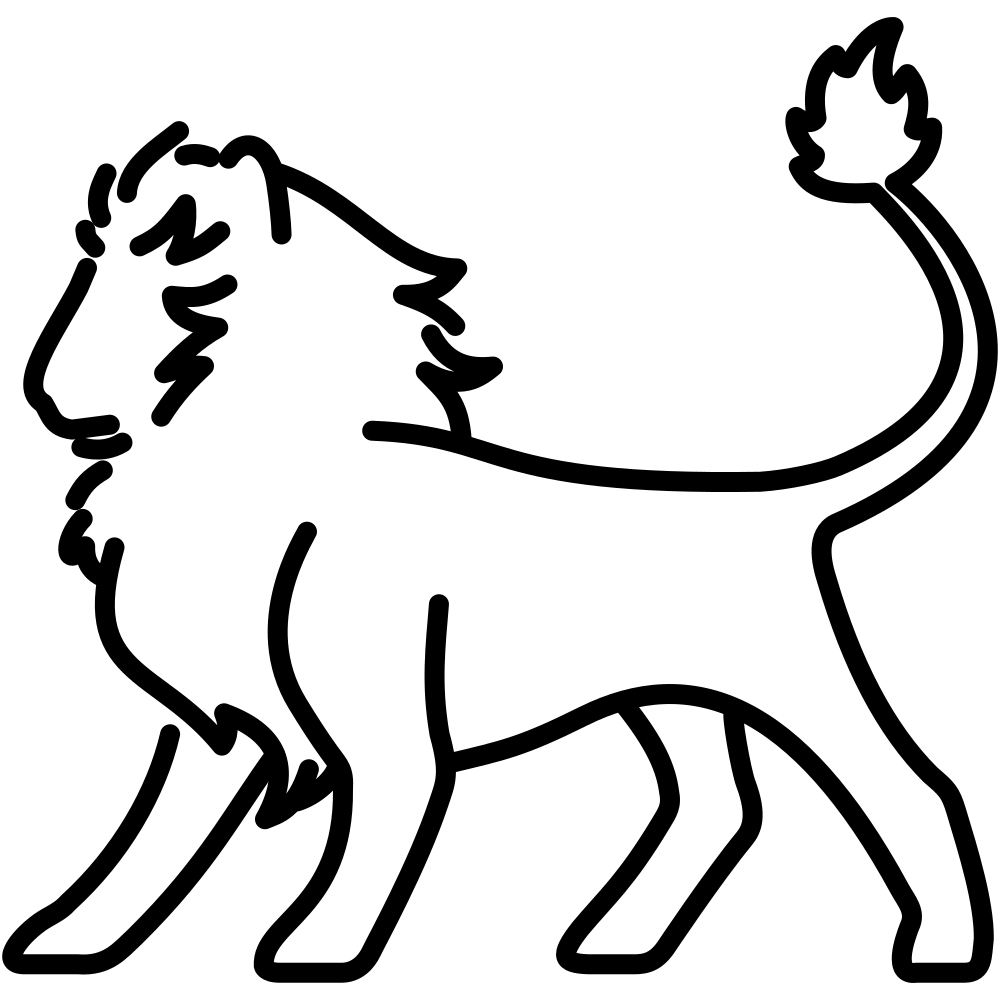
\includegraphics[width=14.57pt,height=15.21pt]{figures/karma_architecture/pettingzoo.png}};
%Straight Lines [id:da5757027637146572] 
\draw [color={rgb, 255:red, 74; green, 144; blue, 226 }  ,draw opacity=1 ][line width=2.25]    (357.9,41) -- (364.9,41) ;
\draw [shift={(352.9,41)}, rotate = 0] [fill={rgb, 255:red, 74; green, 144; blue, 226 }  ,fill opacity=1 ][line width=0.08]  [draw opacity=0] (5.72,-2.75) -- (0,0) -- (5.72,2.75) -- cycle    ;
%Straight Lines [id:da29364722138505184] 
\draw [color={rgb, 255:red, 74; green, 144; blue, 226 }  ,draw opacity=1 ][line width=2.25]    (390.99,97.77) -- (390.99,57.25) ;
\draw [shift={(390.99,52.25)}, rotate = 90] [fill={rgb, 255:red, 74; green, 144; blue, 226 }  ,fill opacity=1 ][line width=0.08]  [draw opacity=0] (5.72,-2.75) -- (0,0) -- (5.72,2.75) -- cycle    ;
%Straight Lines [id:da5470457469462804] 
\draw [color={rgb, 255:red, 74; green, 144; blue, 226 }  ,draw opacity=1 ][line width=2.25]    (390.9,71) -- (325.9,71) ;
\draw [shift={(320.9,71)}, rotate = 360] [fill={rgb, 255:red, 74; green, 144; blue, 226 }  ,fill opacity=1 ][line width=0.08]  [draw opacity=0] (5.72,-2.75) -- (0,0) -- (5.72,2.75) -- cycle    ;
%Shape: Rectangle [id:dp8476965567779329] 
\draw  [color={rgb, 255:red, 255; green, 255; blue, 255 }  ,draw opacity=1 ][fill={rgb, 255:red, 255; green, 255; blue, 255 }  ,fill opacity=1 ] (378.41,65.11) -- (397.83,65.11) -- (397.83,92) -- (378.41,92) -- cycle ;
%Shape: Smiley Face [id:dp8656850497140396] 
\draw  [fill={rgb, 255:red, 255; green, 255; blue, 255 }  ,fill opacity=1 ][line width=0.75]  (380.35,69.4) .. controls (380.35,67.3) and (382.09,65.6) .. (384.24,65.6) .. controls (386.38,65.6) and (388.12,67.3) .. (388.12,69.4) .. controls (388.12,71.5) and (386.38,73.2) .. (384.24,73.2) .. controls (382.09,73.2) and (380.35,71.5) .. (380.35,69.4) -- cycle ; \draw  [fill={rgb, 255:red, 255; green, 255; blue, 255 }  ,fill opacity=1 ][line width=0.75]  (382.53,68.11) .. controls (382.53,67.9) and (382.7,67.73) .. (382.92,67.73) .. controls (383.13,67.73) and (383.31,67.9) .. (383.31,68.11) .. controls (383.31,68.32) and (383.13,68.49) .. (382.92,68.49) .. controls (382.7,68.49) and (382.53,68.32) .. (382.53,68.11) -- cycle ; \draw  [fill={rgb, 255:red, 255; green, 255; blue, 255 }  ,fill opacity=1 ][line width=0.75]  (385.17,68.11) .. controls (385.17,67.9) and (385.34,67.73) .. (385.56,67.73) .. controls (385.77,67.73) and (385.95,67.9) .. (385.95,68.11) .. controls (385.95,68.32) and (385.77,68.49) .. (385.56,68.49) .. controls (385.34,68.49) and (385.17,68.32) .. (385.17,68.11) -- cycle ; \draw  [line width=0.75]  (382.29,70.92) .. controls (383.59,71.94) and (384.88,71.94) .. (386.18,70.92) ;
%Shape: Smiley Face [id:dp9163740789669144] 
\draw  [fill={rgb, 255:red, 255; green, 255; blue, 255 }  ,fill opacity=1 ][line width=0.75]  (392.01,69.4) .. controls (392.01,67.3) and (393.75,65.6) .. (395.89,65.6) .. controls (398.04,65.6) and (399.78,67.3) .. (399.78,69.4) .. controls (399.78,71.5) and (398.04,73.2) .. (395.89,73.2) .. controls (393.75,73.2) and (392.01,71.5) .. (392.01,69.4) -- cycle ; \draw  [fill={rgb, 255:red, 255; green, 255; blue, 255 }  ,fill opacity=1 ][line width=0.75]  (394.18,68.11) .. controls (394.18,67.9) and (394.36,67.73) .. (394.57,67.73) .. controls (394.79,67.73) and (394.96,67.9) .. (394.96,68.11) .. controls (394.96,68.32) and (394.79,68.49) .. (394.57,68.49) .. controls (394.36,68.49) and (394.18,68.32) .. (394.18,68.11) -- cycle ; \draw  [fill={rgb, 255:red, 255; green, 255; blue, 255 }  ,fill opacity=1 ][line width=0.75]  (396.82,68.11) .. controls (396.82,67.9) and (397,67.73) .. (397.21,67.73) .. controls (397.43,67.73) and (397.6,67.9) .. (397.6,68.11) .. controls (397.6,68.32) and (397.43,68.49) .. (397.21,68.49) .. controls (397,68.49) and (396.82,68.32) .. (396.82,68.11) -- cycle ; \draw  [line width=0.75]  (393.95,70.92) .. controls (395.24,71.94) and (396.54,71.94) .. (397.83,70.92) ;
%Shape: Smiley Face [id:dp8186451078369623] 
\draw  [fill={rgb, 255:red, 255; green, 255; blue, 255 }  ,fill opacity=1 ][line width=0.75]  (386.18,77.44) .. controls (386.18,75.34) and (387.92,73.64) .. (390.06,73.64) .. controls (392.21,73.64) and (393.95,75.34) .. (393.95,77.44) .. controls (393.95,79.54) and (392.21,81.24) .. (390.06,81.24) .. controls (387.92,81.24) and (386.18,79.54) .. (386.18,77.44) -- cycle ; \draw  [fill={rgb, 255:red, 255; green, 255; blue, 255 }  ,fill opacity=1 ][line width=0.75]  (388.36,76.15) .. controls (388.36,75.94) and (388.53,75.77) .. (388.74,75.77) .. controls (388.96,75.77) and (389.13,75.94) .. (389.13,76.15) .. controls (389.13,76.36) and (388.96,76.53) .. (388.74,76.53) .. controls (388.53,76.53) and (388.36,76.36) .. (388.36,76.15) -- cycle ; \draw  [fill={rgb, 255:red, 255; green, 255; blue, 255 }  ,fill opacity=1 ][line width=0.75]  (391,76.15) .. controls (391,75.94) and (391.17,75.77) .. (391.39,75.77) .. controls (391.6,75.77) and (391.77,75.94) .. (391.77,76.15) .. controls (391.77,76.36) and (391.6,76.53) .. (391.39,76.53) .. controls (391.17,76.53) and (391,76.36) .. (391,76.15) -- cycle ; \draw  [line width=0.75]  (388.12,78.96) .. controls (389.42,79.98) and (390.71,79.98) .. (392.01,78.96) ;
%Flowchart: Punched Tape [id:dp6020643269389074] 
\draw  [fill={rgb, 255:red, 255; green, 255; blue, 255 }  ,fill opacity=1 ] (313.9,33.81) .. controls (313.9,35.03) and (318.18,36.02) .. (323.45,36.02) .. controls (328.73,36.02) and (333,35.03) .. (333,33.81) .. controls (333,32.58) and (337.28,31.59) .. (342.55,31.59) .. controls (347.83,31.59) and (352.1,32.58) .. (352.1,33.81) -- (352.1,51.52) .. controls (352.1,50.3) and (347.83,49.31) .. (342.55,49.31) .. controls (337.28,49.31) and (333,50.3) .. (333,51.52) .. controls (333,52.75) and (328.73,53.74) .. (323.45,53.74) .. controls (318.18,53.74) and (313.9,52.75) .. (313.9,51.52) -- cycle ;
%Straight Lines [id:da950307097731951] 
\draw [line width=0.75]    (324.14,41.04) -- (341.9,41) ;
%Shape: Smiley Face [id:dp8914579811118104] 
\draw  [line width=0.75]  (320.58,40.88) .. controls (320.58,39.7) and (321.59,38.73) .. (322.85,38.73) .. controls (324.1,38.73) and (325.11,39.7) .. (325.11,40.88) .. controls (325.11,42.07) and (324.1,43.03) .. (322.85,43.03) .. controls (321.59,43.03) and (320.58,42.07) .. (320.58,40.88) -- cycle ; \draw  [line width=0.75]  (321.85,40.15) .. controls (321.85,40.03) and (321.95,39.94) .. (322.08,39.94) .. controls (322.2,39.94) and (322.3,40.03) .. (322.3,40.15) .. controls (322.3,40.27) and (322.2,40.37) .. (322.08,40.37) .. controls (321.95,40.37) and (321.85,40.27) .. (321.85,40.15) -- cycle ; \draw  [line width=0.75]  (323.39,40.15) .. controls (323.39,40.03) and (323.49,39.94) .. (323.62,39.94) .. controls (323.74,39.94) and (323.84,40.03) .. (323.84,40.15) .. controls (323.84,40.27) and (323.74,40.37) .. (323.62,40.37) .. controls (323.49,40.37) and (323.39,40.27) .. (323.39,40.15) -- cycle ; \draw  [line width=0.75]  (321.71,41.74) .. controls (322.47,42.31) and (323.22,42.31) .. (323.98,41.74) ;
%Shape: Smiley Face [id:dp07941198495535606] 
\draw  [line width=0.75]  (329.9,45.15) .. controls (329.9,43.96) and (330.92,43) .. (332.17,43) .. controls (333.42,43) and (334.44,43.96) .. (334.44,45.15) .. controls (334.44,46.33) and (333.42,47.29) .. (332.17,47.29) .. controls (330.92,47.29) and (329.9,46.33) .. (329.9,45.15) -- cycle ; \draw  [line width=0.75]  (331.17,44.42) .. controls (331.17,44.3) and (331.28,44.2) .. (331.4,44.2) .. controls (331.53,44.2) and (331.63,44.3) .. (331.63,44.42) .. controls (331.63,44.54) and (331.53,44.63) .. (331.4,44.63) .. controls (331.28,44.63) and (331.17,44.54) .. (331.17,44.42) -- cycle ; \draw  [line width=0.75]  (332.72,44.42) .. controls (332.72,44.3) and (332.82,44.2) .. (332.94,44.2) .. controls (333.07,44.2) and (333.17,44.3) .. (333.17,44.42) .. controls (333.17,44.54) and (333.07,44.63) .. (332.94,44.63) .. controls (332.82,44.63) and (332.72,44.54) .. (332.72,44.42) -- cycle ; \draw  [line width=0.75]  (331.04,46.01) .. controls (331.79,46.58) and (332.55,46.58) .. (333.3,46.01) ;
%Shape: Smiley Face [id:dp8353415903298282] 
\draw  [line width=0.75]  (341.9,40.85) .. controls (341.9,39.67) and (342.92,38.71) .. (344.17,38.71) .. controls (345.42,38.71) and (346.44,39.67) .. (346.44,40.85) .. controls (346.44,42.04) and (345.42,43) .. (344.17,43) .. controls (342.92,43) and (341.9,42.04) .. (341.9,40.85) -- cycle ; \draw  [line width=0.75]  (343.17,40.12) .. controls (343.17,40) and (343.28,39.91) .. (343.4,39.91) .. controls (343.53,39.91) and (343.63,40) .. (343.63,40.12) .. controls (343.63,40.24) and (343.53,40.34) .. (343.4,40.34) .. controls (343.28,40.34) and (343.17,40.24) .. (343.17,40.12) -- cycle ; \draw  [line width=0.75]  (344.72,40.12) .. controls (344.72,40) and (344.82,39.91) .. (344.94,39.91) .. controls (345.07,39.91) and (345.17,40) .. (345.17,40.12) .. controls (345.17,40.24) and (345.07,40.34) .. (344.94,40.34) .. controls (344.82,40.34) and (344.72,40.24) .. (344.72,40.12) -- cycle ; \draw  [line width=0.75]  (343.04,41.71) .. controls (343.79,42.28) and (344.55,42.28) .. (345.3,41.71) ;
%Straight Lines [id:da21936285199788075] 
\draw [line width=0.75]    (324.19,41.87) -- (329.9,45) ;
%Image [id:dp05694376090002984] 
\draw (218.44,70.24) node  {
\includegraphics[width=18.66pt,height=18.36pt]{figures/karma_architecture/api.png}};
%Image [id:dp7747210194064744] 
\draw (186.74,54.54) node  {
\includegraphics[width=18.66pt,height=18.36pt]{figures/karma_architecture/deploy.png}};
%Image [id:dp5268588430037433] 
\draw (186.74,87.76) node  {
\includegraphics[width=18.66pt,height=18.36pt]{figures/karma_architecture/deploy.png}};
%Image [id:dp7447308292951857] 
\draw (218.44,111.76) node  {
\includegraphics[width=18.66pt,height=18.36pt]{figures/karma_architecture/prometheus.png}};
%Shape: Rectangle [id:dp7837974954754439] 
\draw  [color={rgb, 255:red, 75; green, 101; blue, 225 }  ,draw opacity=1 ][fill={rgb, 255:red, 74; green, 144; blue, 226 }  ,fill opacity=1 ] (202.37,94.64) -- (208.29,94.64) -- (208.29,101.67) -- (202.37,101.67) -- cycle ;
%Shape: Rectangle [id:dp780870970882084] 
\draw  [color={rgb, 255:red, 75; green, 101; blue, 225 }  ,draw opacity=1 ][fill={rgb, 255:red, 74; green, 144; blue, 226 }  ,fill opacity=1 ] (286.37,126) -- (292.29,126) -- (292.29,133.03) -- (286.37,133.03) -- cycle ;

%Shape: Rectangle [id:dp7051683429553395] 
\draw  [color={rgb, 255:red, 75; green, 101; blue, 225 }  ,draw opacity=1 ][fill={rgb, 255:red, 74; green, 144; blue, 226 }  ,fill opacity=1 ] (397.37,124.64) -- (403.29,124.64) -- (403.29,131.67) -- (397.37,131.67) -- cycle ;

%Shape: Rectangle [id:dp5578959475333973] 
\draw  [color={rgb, 255:red, 75; green, 101; blue, 225 }  ,draw opacity=1 ][fill={rgb, 255:red, 74; green, 144; blue, 226 }  ,fill opacity=1 ] (368.37,54.64) -- (374.29,54.64) -- (374.29,61.67) -- (368.37,61.67) -- cycle ;

%Shape: Rectangle [id:dp2822949836407178] 
\draw  [color={rgb, 255:red, 75; green, 101; blue, 225 }  ,draw opacity=1 ][fill={rgb, 255:red, 74; green, 144; blue, 226 }  ,fill opacity=1 ] (324.37,78) -- (330.29,78) -- (330.29,85.03) -- (324.37,85.03) -- cycle ;

%Shape: Rectangle [id:dp9339299822588341] 
\draw  [color={rgb, 255:red, 75; green, 101; blue, 225 }  ,draw opacity=1 ][fill={rgb, 255:red, 74; green, 144; blue, 226 }  ,fill opacity=1 ] (205.37,48) -- (211.29,48) -- (211.29,55.03) -- (205.37,55.03) -- cycle ;



% Text Node
\draw (205.5,98.5) node  [font=\fontsize{0.33em}{0.4em}\selectfont,color={rgb, 255:red, 255; green, 255; blue, 255 }  ,opacity=1 ] [align=left] {1};
% Text Node
\draw (244,58.5) node  [font=\normalsize] [align=left] {{\tiny Scaling}};
\draw (244,64.5) node  [font=\normalsize] [align=left] {{\tiny actions}};
% Text Node
\draw (244,99.5) node  [font=\normalsize] [align=left] {{\tiny Metrics}};
\draw (244,105.5) node  [font=\normalsize] [align=left] {{\tiny data}};
% Text Node
\draw (344.5,36) node  [font=\fontsize{0.33em}{0.4em}\selectfont] [align=left] {\begin{minipage}[lt]{8.66pt}\setlength\topsep{0pt}
\begin{center}
{\fontsize{0.33em}{0.4em}\selectfont $\displaystyle \mathbf{\textcolor[rgb]{0.82,0.01,0.11}{\pi }\textcolor[rgb]{0.82,0.01,0.11}{_{3}}}$}
\end{center}

\end{minipage}};
% Text Node
\draw (341,46.5) node  [font=\fontsize{0.33em}{0.4em}\selectfont] [align=left] {\begin{minipage}[lt]{8.66pt}\setlength\topsep{0pt}
\begin{center}
{\fontsize{0.33em}{0.4em}\selectfont $\displaystyle \mathbf{\textcolor[rgb]{0.82,0.01,0.11}{\pi }\textcolor[rgb]{0.82,0.01,0.11}{_{2}}}$}
\end{center}

\end{minipage}};
% Text Node
\draw (320.9,48) node  [font=\fontsize{0.33em}{0.4em}\selectfont] [align=left] {\begin{minipage}[lt]{8.66pt}\setlength\topsep{0pt}
\begin{center}
{\fontsize{0.33em}{0.4em}\selectfont $\displaystyle \mathbf{\textcolor[rgb]{0.82,0.01,0.11}{\pi }\textcolor[rgb]{0.82,0.01,0.11}{_{1}}}$}
\end{center}

\end{minipage}};
% Text Node
\draw  [color={rgb, 255:red, 75; green, 101; blue, 225 }  ,draw opacity=1 ][fill={rgb, 255:red, 136; green, 197; blue, 246 }  ,fill opacity=1 ][line width=1.5]   (322.77,14.89) .. controls (322.77,13.78) and (323.67,12.89) .. (324.77,12.89) -- (355.77,12.89) .. controls (356.88,12.89) and (357.77,13.78) .. (357.77,14.89) -- (357.77,26.89) .. controls (357.77,27.99) and (356.88,28.89) .. (355.77,28.89) -- (324.77,28.89) .. controls (323.67,28.89) and (322.77,27.99) .. (322.77,26.89) -- cycle  ;
\draw (340.27,20.89) node  [font=\tiny] [align=left] {\begin{minipage}[lt]{21.5pt}\setlength\topsep{0pt}
\begin{center}
KARMA
\end{center}

\end{minipage}};
% Text Node
\draw (290,40.5) node  [font=\tiny] [align=left] {\begin{minipage}[lt]{27.24pt}\setlength\topsep{0pt}
\begin{center}
Organizational\\Analysis
\end{center}

\end{minipage}};
% Text Node
\draw (388,86.39) node  [font=\tiny] [align=left] {\begin{minipage}[lt]{43.42pt}\setlength\topsep{0pt}
\begin{center}
Trained policies
\end{center}

\end{minipage}};
% Text Node
\draw (344.13,127.35) node  [font=\tiny] [align=left] {\begin{minipage}[lt]{60.78pt}\setlength\topsep{0pt}
\begin{center}
PettingZoo environment
\end{center}

\end{minipage}};
% Text Node
\draw (218,127) node  [font=\tiny] [align=left] {\begin{minipage}[lt]{30.31pt}\setlength\topsep{0pt}
\begin{center}
Prometheus
\end{center}

\end{minipage}};
% Text Node
\draw  [color={rgb, 255:red, 75; green, 101; blue, 225 }  ,draw opacity=1 ][fill={rgb, 255:red, 136; green, 197; blue, 246 }  ,fill opacity=1 ][line width=1.5]   (272.9,62) .. controls (272.9,60.9) and (273.8,60) .. (274.9,60) -- (317.9,60) .. controls (319.01,60) and (319.9,60.9) .. (319.9,62) -- (319.9,83) .. controls (319.9,84.1) and (319.01,85) .. (317.9,85) -- (274.9,85) .. controls (273.8,85) and (272.9,84.1) .. (272.9,83) -- cycle  ;
\draw (296.4,72.5) node  [font=\tiny,color={rgb, 255:red, 0; green, 0; blue, 0 }  ,opacity=1 ] [align=left] {Transfer\\Component};
% Text Node
\draw  [color={rgb, 255:red, 75; green, 101; blue, 225 }  ,draw opacity=1 ][fill={rgb, 255:red, 136; green, 197; blue, 246 }  ,fill opacity=1 ][line width=1.5]   (365.88,29.46) .. controls (365.88,28.35) and (366.78,27.46) .. (367.88,27.46) -- (410.88,27.46) .. controls (411.99,27.46) and (412.88,28.35) .. (412.88,29.46) -- (412.88,50.46) .. controls (412.88,51.56) and (411.99,52.46) .. (410.88,52.46) -- (367.88,52.46) .. controls (366.78,52.46) and (365.88,51.56) .. (365.88,50.46) -- cycle  ;
\draw (389.38,39.96) node  [font=\tiny,color={rgb, 255:red, 0; green, 0; blue, 0 }  ,opacity=1 ] [align=left] {Analyzing\\Component};
% Text Node
\draw  [color={rgb, 255:red, 75; green, 101; blue, 225 }  ,draw opacity=1 ][fill={rgb, 255:red, 136; green, 197; blue, 246 }  ,fill opacity=1 ][line width=1.5]   (365.88,98.24) .. controls (365.88,97.13) and (366.78,96.24) .. (367.88,96.24) -- (410.88,96.24) .. controls (411.99,96.24) and (412.88,97.13) .. (412.88,98.24) -- (412.88,119.24) .. controls (412.88,120.34) and (411.99,121.24) .. (410.88,121.24) -- (367.88,121.24) .. controls (366.78,121.24) and (365.88,120.34) .. (365.88,119.24) -- cycle  ;
\draw (389.38,108.74) node  [font=\tiny,color={rgb, 255:red, 0; green, 0; blue, 0 }  ,opacity=1 ] [align=left] {Training\\Component};
% Text Node
\draw (172.5,33.36) node  [font=\tiny] [align=left] {\begin{minipage}[lt]{16.92pt}\setlength\topsep{0pt}
\begin{center}
Cluster
\end{center}

\end{minipage}};
% Text Node
\draw  [color={rgb, 255:red, 75; green, 101; blue, 225 }  ,draw opacity=1 ][fill={rgb, 255:red, 136; green, 197; blue, 246 }  ,fill opacity=1 ][line width=1.5]   (272.9,99) .. controls (272.9,97.9) and (273.8,97) .. (274.9,97) -- (317.9,97) .. controls (319.01,97) and (319.9,97.9) .. (319.9,99) -- (319.9,120) .. controls (319.9,121.1) and (319.01,122) .. (317.9,122) -- (274.9,122) .. controls (273.8,122) and (272.9,121.1) .. (272.9,120) -- cycle  ;
\draw (296.4,109.5) node  [font=\tiny,color={rgb, 255:red, 0; green, 0; blue, 0 }  ,opacity=1 ] [align=left] {Modeling\\Component};
% Text Node
\draw (173,73.72) node  [font=\tiny,rotate=-90] [align=left] {{\LARGE {\fontfamily{helvet}\selectfont \textcolor[rgb]{0.29,0.56,0.89}{...}}}};
% Text Node
\draw (125.61,118.47) node  [font=\tiny] [align=left] {{\LARGE {\fontfamily{helvet}\selectfont \textcolor[rgb]{0.29,0.56,0.89}{...}}}};
% Text Node
\draw (147,89.5) node  [font=\tiny,rotate=-90] [align=left] {{\LARGE {\fontfamily{helvet}\selectfont \textcolor[rgb]{0.29,0.56,0.89}{...}}}};
% Text Node
\draw (125.61,59.9) node  [font=\tiny] [align=left] {{\LARGE {\fontfamily{helvet}\selectfont \textcolor[rgb]{0.29,0.56,0.89}{...}}}};
% Text Node
\draw (208.5,51.86) node  [font=\fontsize{0.33em}{0.4em}\selectfont,color={rgb, 255:red, 255; green, 255; blue, 255 }  ,opacity=1 ] [align=left] {6};
% Text Node
\draw (327.5,81.86) node  [font=\fontsize{0.33em}{0.4em}\selectfont,color={rgb, 255:red, 255; green, 255; blue, 255 }  ,opacity=1 ] [align=left] {5};
% Text Node
\draw (371.5,58.5) node  [font=\fontsize{0.33em}{0.4em}\selectfont,color={rgb, 255:red, 255; green, 255; blue, 255 }  ,opacity=1 ] [align=left] {4};
% Text Node
\draw (400.5,128.5) node  [font=\fontsize{0.33em}{0.4em}\selectfont,color={rgb, 255:red, 255; green, 255; blue, 255 }  ,opacity=1 ] [align=left] {3};
% Text Node
\draw (289.5,129.86) node  [font=\fontsize{0.33em}{0.4em}\selectfont,color={rgb, 255:red, 255; green, 255; blue, 255 }  ,opacity=1 ] [align=left] {2};


\end{tikzpicture}
    \caption{Overview of the KARMA framework in use with a Kubernetes cluster}
    \label{fig:karma_architecture}
\end{figure}

As illustrated in \autoref{fig:karma_architecture}, the KARMA framework operates alongside the Kubernetes cluster, comprising \textbf{worker nodes} that host \textbf{pods} (the atomic unit in Kubernetes containing \textbf{containers} running the actual processes). Pods are organized into \textbf{services} and managed by \textbf{deployments} to update the number of pod refered to as \textbf{replica}. The KARMA framework functions as a separate software layer, interfacing with both the Kubernetes API and Prometheus.

\textbf{1)} Metrics related to availability are gathered as states by \textit{Prometheus}~\cite{prometheus}, a widely adopted time-series metrics database, and processed by KARMA's \textbf{Modeling Component}.

\textbf{2)} Collected states are used to construct a \textit{digital twin} of the cluster as a state transition model. A reward function, defined as a weighted sum of QoS-specific sub-rewards, drives the operational resilience. The digital twin provides a controlled simulation environment to train agents safely without risking disruptions in the real cluster.

\textbf{3)} The \textbf{Training Component} trains agents to maximize rewards to improve operational resilience. Agents are optionally guided by \textit{roles} (constraints shaping their actions) and \textit{missions} (incremental goals facilitating policy convergence), following the AOMEA methodology~\cite{soule2024aomea}.

\textbf{4)} The \textbf{Analyzing Component} visualize the learned policies through trajectory clustering and hierarchical visualization, ensuring interpretability, alignment with goals, and resilience to dynamic workloads.

\textbf{5)} The \textbf{Transfer Component} deploys trained policies to the real Kubernetes cluster via the Kubernetes API, executing replica adjustments \textbf{(6)}. Continous interactions between agents and the cluster enables enriching the digital twin with newly collected traces, eventually updating the agents' policy regularly to meet environment's changes.

KARMA integrates simulation-based learning with real-world Kubernetes operations in a closed-loop process. Metrics collected from the cluster guide policy updates, while trained agents' decisions are applied back to the cluster. This iterative process aims to ensure ongoing adaptability, robustness, and resilience under diverse conditions.


\subsubsection{Modeling}
% Modeling:
%  - observation
%  - actions
%  - rewards -> Faire une récompense qui englobe toutes les QoS ayant pour père la QoS (ne pas faire encore référence aux fonctions de récompense pour l'instant) "availability"
%  - transition -> Transition modeling + MLP -> donner détails des paramètres

In this activité, we assume the initial defender and attacker agents have applied various action in the cluster, leading to a collection of representative amount of traces. Relying on the formalization of the environment as a zero-sum \textbf{Stochastic Game (SG)}~\cite{shapley1953stochastic}, we can provide a near-realistic simulation environment from these collected traces. The SG is characterized by the tuple $\mathcal{SG} = (\mathcal{A}, S, A, T, R, \gamma)$, where $\mathcal{A} = \{\mathcal{A}_d, \mathcal{A}_a\}$ is the agents set comprising $n = |\mathcal{A}_d|$ defender agents and one single attacker agent in $\mathcal{A}_a$; and $\gamma \in [0, 1]$ is the discount factor for future rewards.

\noindent \paragraph{\textbf{State Space}} $S$ is the state space of the Kubernetes cluster. A state denoted as $s \in S$, consists of metrics to characterizing system performance for each of the $d = |D|$ micro-service deployments:
$$
s = (n_{id}, d_{dep}, d_{des}, d_{err}, d_{rem}, r_{cpu}, r_{ram}, t_{in}, t_{out})^d
$$
$n_{id} \in \mathbb{N}$: the deployment number; \quad
$d_{dep} \in \mathbb{N}$: the number of deployed pods; \quad 
$d_{des} \in \mathbb{N}$: the number of desired pods; \quad
$d_{err} \in \mathbb{N}$: the number of failed pods; \quad
$d_{rem} \in \mathbb{N}$: the number of remaining requests to be processed in the queue; \quad
$r_{cpu} \in \mathbb{R}$: the total aggregated CPU (in m) of the pods; \quad
$r_{ram} \in \mathbb{R}$: the total aggregated memory (in Mi) of the pods; \quad
$t_{in} \in \mathbb{R}$: the average received traffic (in Kbps); \quad
$t_{out} \in \mathbb{R}$: the average transmitted traffic (in Kbps).
% TODO: ajouter les métriques spécifiques pour pouvoir vérifier s'il y a des goulots d'étranglement, 

% These metrics are continuously collected using Prometheus~\cite{prometheus}, a widely adopted monitoring and metrics database system, enabling the capture of time-series data for each pod, deployment, and the cluster as a whole.

\noindent \paragraph{\textbf{Action Space}} $A = A_d^n \times A_a$ is the action space with $A_d$ and $A_a$ are the action spaces for a defender and the attacker agents respectively:

\vspace{0.3cm}

\indent\begin{minipage}{0.15\linewidth}
    (1)
\end{minipage}
\begin{minipage}{0.9\linewidth}
    \raggedright
    $\displaystyle a_d \in A_d = (service\_id, replica\_change)$
\end{minipage}

\vspace{0.3cm}

\indent $\mathbf{service\_id} \in \mathbb{N}$ identifies the target service (through deployment), and $\mathbf{replica\_change} \in [-\alpha, +\alpha]$ indicates the change as for pod replica number. Actions from this space are one-hot encoded as a Box Gym Space~\cite{openAIGymActionSpaces}: for example, the defender actions $(2,1)$, $(0,-2), (1,0)$ mean the services with id numbers equal to $2$, $0$, and $1$ have their respective replica numbers changed by adding $1$, $-2$, $0$.

\

\indent\begin{minipage}{0.06\linewidth}
    (2)
\end{minipage}
\begin{minipage}{0.9\linewidth}
    \raggedright
    $\displaystyle a_a \in A_a = (\text{entry\_point\_id}, \text{rate\_change}, \text{data\_change})$
\end{minipage}

\vspace{0.3cm}

\indent $\mathbf{entry\_point\_id} \in \mathbb{N}$ specifies the service entry point;
$\mathbf{rate\_change} \in \{\textit{high\_decrease}, \textit{low\_decrease}, \textit{no\_change}, \allowbreak \textit{low\_increase}, \allowbreak \textit{high\_increase}\}$ changes the incoming traffic based on a factor $\kappa$; and $\mathbf{data\_change} \in \{\textit{no\_alteration}, \allowbreak \textit{low\_alteration}, \allowbreak \textit{high\_alteration}\}$ specifies the degree of data alteration based on factor $\sigma \in [2,\infty[$. Actions from this space are one-hot encoded as a Box Gym space: for example, the attacker actions $(0,1,2), (2,-1,0), (1,2,1)$ mean that entrypoint services id number 0, 2, and 1 would have their respective traffic-in rates increased by $1 \times \kappa, -1 \times \kappa, 2 \times \kappa$, and respective probabilities to crash due to data alteration are changed by $\frac{2}{\sigma}, \frac{0}{\sigma}, \frac{1}{\sigma}$.


\noindent \paragraph{\textbf{Reward Functions}} $R = \{R_d, R_a\}$, with $R_d: S \times A \to \mathbb{R}$ and $R_a: S \times A \to \mathbb{R} = - R_d$ are respectively the reward function for the defender agents based on operational resilience and the attacker one.
To measure operational resilience, we use the linear combination of the following metrics:
%
\begin{itemize}
    \vspace{0.15cm}
    \item $\text{Success Rate } (sr) : \frac{\text{Successful Requests}}{\text{Total Received Requests}}$
    \vspace{0.15cm}
    \item $\text{Pod Failure Rate } (pfr) : \frac{\text{Failed Pods}}{\text{Total Deployed Pods}}$
    \vspace{0.15cm}
    \item $\text{Latency Ratio } (lr) : \min\left(1,\frac{\text{Measured Latency}}{\text{Maximum Acceptable Latency}}\right)$
    \vspace{0.15cm}    
    \item $\text{Entry Point Availability } (epa) : \frac{\text{Available Entry Points}}{\text{Total Entry Points}}$
    \vspace{0.15cm}
    \item $\text{Traffic Capacity Ratio } (tcr) : \min\left(1, \frac{\text{Outgoing Traffic}}{\text{Expected Traffic}}\right)$
\end{itemize}

\vspace{0.3cm}

$\text{Operational Resilience }: or(s) = w_1 \times sr
\allowbreak + w_2 \times (1 - pfr)
\allowbreak + w_3 \times (1 - lr)
\allowbreak + w_4 \times epa
\allowbreak + w_5 \times tcr
\text{ where } (w_1, w_2, w_3, w_4, w_5) \text{ are relative weights.}$

\

Then, the reward function is formalized as follow:

$$
\begin{cases} 
    R_a(s, a_d, a_a) = -R_d(s, a_d, a_a) & \\
    R_a(s, a_d, a_a) = or(s)
\end{cases}
$$

where $s$ is the current state after applying actions, and the weights $(w_1, w_2, w_3, w_4, w_5)$ are empirically tuned to favor a balanced global functioning in the cluster.


\noindent \paragraph{\textbf{Transition Modeling}} $T: S \times A \rightarrow S$ is the real state transition function dictating the next state when the joint actions of the defender agents and the attacker's one are applied. Relying a representative set of collected transitions $\mathcal{T} = \langle(s, a_d^n, a_a, s')_{t\in \mathbb{N}}\rangle$ over a time window, we can form a partial state transition function $\hat{T}_t$ defined as:
%
$$
\hat{T}_t(s, a_d^n, a_a) =
\begin{cases} 
    s' & \text{if } (s, a_d^n, a_a, s') \in \mathcal{T} \\
    \emptyset & \text{ otherwise}
\end{cases}
$$

To cover no recorded transition, we introduce a Multi-Layer Perceptron (MLP)-based approximator $\hat{T}_a$ to learn from collected transitions and predict the next likely state. The choice of an MLP is motivated by its universal approximation capabilities and the assumption that the next state of a Kubernetes cluster depends only on the current state and the chosen actions. This assumption holds because:
\begin{enumerate}[label={\roman*)}, itemjoin={;\quad }]
    \item Kubernetes autoscaling decisions are primarily dictated by real-time resource metrics (CPU, memory, network) which do not depend on historical states beyond a small time window
    \item Previous works in reinforcement learning for autoscaling~\cite{Gari2021} have demonstrated that Markovian models effectively approximate real-world cluster behavior.
\end{enumerate}
The MLP approximator has three hidden layers, striking a balance between expressiveness and computational efficiency. The input and output layer dimensions correspond to the size of the state space, while each hidden layer consists of 128 neurons. Rectified Linear Unit (ReLU) activation functions are applied to the hidden layers, and a linear activation function is used at the output layer to produce the predicted next state. The model is optimized using the Adam optimizer with a learning rate of $10^{-3}$, minimizing the Mean Squared Error loss function, expressed as
$$
\mathcal{L} = \frac{1}{N} \sum_{i=1}^N |T(s_i, a_{d,i}, a_{a,i}) - s'_i|^2
$$
where $N$ is a number of representative transitions to ensure generalization.

The complete modeled transition function $\hat{T}$ is defined as:
$$
\hat{T}(s, a_d, a_a) = 
\begin{cases} 
\hat{T}_t(s, a_d, a_a) & \text{if } (s, a_d, a_a) \in \text{Domain}(\hat{T}_t), \\
\hat{T}_a(s, a_d, a_a) & \text{otherwise}.
\end{cases}
$$

\noindent \paragraph{\textbf{Digital Twin Environment}} The defined action and state spaces with the approximated transition function $\hat{T}$, combined with the reward functions $R_d$ and $R_a$, forms the basis of the digital twin environment implemented using the PettingZoo library~\cite{Terry2021}. This environment enables simulating the cluster from the defined SG, offering a safe space for defender agents to explore various strategies against the attacker agent.



\subsubsection{Training}
\label{sec:training}

In this activité, MARL algorithms are applied within the modeled environment to enable agents to learn by maximizing cumulative rewards. As suggested in AOMEA~\cite{soule2024aomea}, we leverage the $\mathcal{M}OISE^+$ organizational model to bring ways to control/guide the MARL training. In the KARMA framework it results in a decomposition of the overarching goal of \textit{operational resilience} into sub-goals. Each sub-goal is assigned to a specific agent as a mission, while roles define rule-based strategies to guide agent operations.\\

\noindent \textbf{Agent Roles and Missions}

\

A \textbf{role} is formally represented by a \textbf{Role Action Guide} (RAG), which restricts an agent's permissible actions:
$$
rag(h, \omega) = (\{a_1, a_2, \dots, a_i\}, ch)
$$
where $h$ represents the trajectory or history, \(\omega\) is the agent's observation, and \(ch \in \{0,1\}\) is the constraint hardness. A hard constraint (\(ch = 1\)) strictly limits the agent's available actions to authorized ones, while a soft constraint (\(ch = 0\)) allows for exploratory actions but adjusts rewards with bonuses or penalties based on compliance with the authorized action set. For example, the \textit{Bottleneck Manager} has a role restricting its actions to modifying pod replicas within a specific service graph, ensuring it does not affect unrelated services. If a bottleneck is detected in Service A that causes delays in Service B, the agent adheres to its role by increasing the pod replicas of Service A to resolve the issue without overstepping constraints.

\

A \textbf{mission} is a set of intermediate goals designed to assist in achieving the overarching operational resilience goal. A goal is represented by a \textbf{Goal Reward Guide} (GRG), which incentivizes achieving the expected outcome for this goal:
$$
grg(h) = r_b,
$$
where \(h \in H\) represents the current agent trajectory and \(r_b \in \mathbb{R}\) is the associated reward bonus or penalty. This mechanism narrows the optimization focus to critical resilience tasks. For instance, the \textit{DDoS Manager} is assigned a mission to maintain service availability during DDoS attacks. It earns a reward bonus for ensuring that a predefined percentage of incoming requests is successfully handled, despite the increased load, by dynamically adjusting replicas. The mission aligns the agent's focus on balancing load while avoiding resource over-provisioning.\\

By defining specific \textbf{(role, mission)} pairs, the KARMA framework assigns specialized tasks to agents to tackle distinct challenges in chained Kubernetes services. These roles and missions enable distributed yet coordinated policy learning, ensuring that agents align their actions to maximize overall \textit{operational resilience}. For example, while the \textit{Bottleneck Manager} alleviates bottlenecks to ensure steady service throughput, its actions complement those of the \textit{DDoS Manager}, which adjusts replicas to mitigate traffic surges. This interdependence highlights the importance of coordinating roles and missions to address shared challenges.

\paragraph*{Algorithms and training pipeline}

KARMA integrates \textit{Multi-Agent Proximal Policy Optimization}~\cite{Yu2022} (MAPPO), an Actor-Critic MARL algorithm where the centralized critic provides global feedback, helping agents learn cooperative strategies by optimizing a shared value function. Meanwhile, decentralized actors ensure independent decision-making, preserving realistic execution. This structure fosters emergent collaboration as agents implicitly coordinate through the centralized learning process~\cite{Yu2022}, which is critical in KARMA due to the interdependencies between roles and missions.

The training pipeline in KARMA follows a systematic sequence to optimize agent behaviors. Initially, policies (\(\pi_i\)), roles (RAG), and missions (GRG) are defined for all agents to establish a structured framework. Agents participate in simulation runs, generating trajectories within the digital twin environment. At each step, roles with hard constraints restrict the available actions to authorized ones, while soft constraints influence rewards by applying bonuses or penalties based on compliance. Missions add further reward shaping by incentivizing goal-aligned trajectories. The \textit{Optuna}~\cite{akiba2019optuna} framework is used for Hyper-Parameter Optimization, iteratively refining policies by adjusting hyperparameters and role specifications to improve convergence and enhance system resilience.

Convergence is deemed successful when the standard deviation of cumulative rewards across episodes falls below a predefined threshold $\mu \in \mathbb{R}$, and cumulative rewards exceed an empirically determined minimum value $\lambda \in \mathbb{R}$.


\subsubsection{Analysis}
\label{sec:analysis}

This activité aims to interpret agent behaviors as understandable roles and goals, particularly in dynamic, unstructured environments where loosely defined roles and goals lead to broad policy convergence. More complexity arises when agents must coordinate, as in DDoS scenarios, where prioritization emerges implicitly. Understanding these interactions can help ensuring structured coordination and optimal policy convergence~\cite{Shoham2009MAS}.

We propose a manual post-training method to analyze the trajectories of trained agents (comparable to sequences of actions) using unsupervised learning techniques to identify roles, missions, and inter-agent interactions based on a general definition of each, derived from their trajectories.

We also envisioned this method to reduce reliance on domain-specific knowledge by framing role and goal design as an optimization problem, where agent policies evolve within a policy space that is iteratively refined. Training begins with minimal constraints, allowing efficient behaviors to emerge, revealing abstract roles and goals that progressively narrow the search space. With each iteration, newly identified roles and goals further restrict the space, improving precision. Through repeated training, analysis, and refinement, this process aims to design relevant, domain-agnostic roles and goals with minimal manual intervention, enhancing KARMA's generalizability.

\paragraph*{\textbf{Identifying Roles}}

We propose that agents sharing the same role should exhibit similar trajectories. To identify recurring action sequences that define a common role among agents, we apply hierarchical clustering. The distance between these sequences is computed using Dynamic Time Warping~\cite{berndt1994using} (DTW), allowing for variations in timing across test episodes:
\[
d(\tau_i, \tau_j) = \min_{\pi} \sum_{k=1}^{|\pi|} \|a_{t_k}^i - a_{t_k}^j\|_2,
\]
where $\pi$ is the optimal alignment path. Clustering hyperparameters, such as the number of clusters, are empirically tuned to minimize noise and avoid generating rough roles. Clusters are annotated to define abstract roles if they do not match existing ones, such as \textit{Bottleneck Manager} or \textit{DDoS Manager}.

\paragraph*{\textbf{Identifying Missions}}

We propose that agents sharing the same goal should transition through at least one similar state, though possibly via different paths. To identify such similar states, we leverage K-means clustering to group trajectories of performing agents based on the similarity of visited states. Similar states in a cluster are used to define intermediate goals:
\[
g_i = \mathcal{S}_j, \quad \text{where } \mathcal{S}_j = \{s \in \tau_i | \mathbb{P}(s) > \epsilon\}.
\]
Here, $\mathbb{P}(s)$ represents the probability of visiting a state $s$ within successful trajectories. $\epsilon$ represents a threshold used to filter states $s$ based on their probability $\mathbb{P}(s)$ of being visited to minimize noise. Hyperparameters of K-means are empirically optimized to minimize noise. Sampled states are annotated to define abstract goals if they do not match existing ones.


\paragraph*{\textbf{Identifying Inter-Agent Interactions}}

Explainability in KARMA also requires an understanding of how agents coordinate their actions in different contexts. This is achieved by analyzing inter-agent relationships using the concepts of $\mathcal{M}OISE^+$~\cite{hubner2002moise}, which formalizes relations such as:
\begin{enumerate}[label=\textbf{\arabic*)}, itemjoin={;\quad }]
    \item \textbf{Acquaintance Relations}: Derived from shared observations or reward signals during training, these relations represent which agents are aware of each other's actions.
    \item \textbf{Authority Relations}: Captured through dependency patterns, authority relations prioritize one agent's decisions over another's in specific scenarios. For instance, an specific agent may hold authority during a DDoS attack.
    \item \textbf{Communication Relations}: Inferred from synchronized actions or information-sharing events. For example, agents sharing traffic load data to coordinate replica adjustments during surges.
\end{enumerate}

To visualize these relations, a directed graph can be constructed where nodes represent agents and edges represent relations, annotated with interaction type on a time window.
%Considering a time window, we can generate a graph based on detected relations and may evolves dynamically on the next time window, highlighting changes in interaction patterns.

% In addition, we also determine the \textbf{patterns of coordination} that aim to understand the mutual impact of an agent's actions onto another agent's trajectory  over time. Among Sequential Pattern Mining, we favoured the use of the \textit{PrefixSpan} algorithm to identify recurring action sequences across agents during specific scenarios. For example, patterns may show that one agent defers actions to another during adversarial conditions. Detected sequences can be represented as a sequence diagram illustrates how agents interact over time, showing causal relationships and dependencies in resolving challenges.



\subsubsection{Transfer}
\label{sec:transfer}

% Transfering: Processus de transfert des comportements appris au cluster réel.
%  - récupérer les politiques entrainés dans un sous-module
%  - lancer les politiques entrainés avec l'état courant collecté
%  - appliquer les actions choisies par ces politiques via l'API K8s

In this activité, policies interact with the real cluster:
\begin{enumerate}[label=\textbf{\arabic*)}, itemjoin={;\quad }]
    \item \textbf{State Collection:} Real-time metrics such as CPU usage, memory consumption, pod status, and network traffic are collected from the Prometheus server~\cite{prometheus}
    \item \textbf{Policy Execution:} Each agent's policy $\pi_i$ computes an action $a_t^i$ based on the current state $s_t$, selecting adjustments such as scaling pod replicas for a deployment
    \item \textbf{Action Application:} The computed actions are sent as API requests, directly modifying deployment.
\end{enumerate}

Agents in the transfer component continuously interact with the Kubernetes API, generating states that are stored in the modeling component's database. Initially, a large time window is used to collect representative traces for creating a near-realistic digital twin of the Kubernetes cluster. Subsequently, at shorter regular intervals, the modeling component updates the digital twin using the latest trace data. This iterative process aims to ensure agents dynamically adapt to workload.


%
% The agents interact seamlessly with Kubernetes:
% \begin{enumerate}[label={}, itemjoin={;\quad }]
%     \item Actions are applied to deployments via the API
%     \item Real-time metrics are gathered using Prometheus, ensuring up-to-date cluster state observations
%     \item KARMA operates independently of the native Kubernetes HPA mechanisms.
% \end{enumerate}

% \

% \noindent The framework integrates a feedback loop:
% \begin{enumerate}[label=\textbf{\arabic*)}, itemjoin={;\quad }]
%     \item Metrics from the live cluster are used to update the digital twin model.
%     \item Agents are periodically retrained on this updated model to refine their policies for new workload patterns or adversarial conditions.
%     \item Refined policies are redeployed to the cluster, maintaining high adaptability and resilience.
% \end{enumerate}

\footnotetext[1]{\label{lnk:footnote_1}Source code available with extra details at: \url{https://anonymous.4open.science/r/KARMA-040B/README.md}}

% =======================================
\subsection{Experimental Setup}
\label{sec:experiments}
% Experimental setup:
%  - Présenter "Chained Services"
%  - CybMASDE: présenter comme un moyen d'implémenter KARMA et présenter la configuration logicielle
%  - Configuration matérielle (pour entrainement et analyse)
%  - Protocole d'experimentation et d'analyse (prend en compte un espèce d'étude d'ablation dans les baselines)
%  - Métriques d'évaluation
%  - Baselines: MA x (Org. Spec.)
%     - modèle sans specifications organisationnelles avec 1 seul agent (état de l'art)
%     - modèle avec spécifications organisationnelles du modèle "fort" avec 1 seul agent (état de l'art?)
%     - modèle sans spécifications organisationnelles avec plusieurs agents (état de l'art?)
%     - modèle avec spécifications organisationnelles du modèle "faible" avec plusieurs agents
%     - modèle avec spécifications organisationnelles du modèle "fort" avec plusieurs agents

This section outlines the experimental setup for evaluating KARMA's ability to address initially defined gaps.

\subsubsection{Description of the Kubernetes Cluster and Configuration}

The evaluation environment consists of a Kubernetes cluster simulating a \textbf{Chained Services} (CS) architecture. Each service comprises a set of microservices hosted in pods and managed by deployments. For instance, \autoref{fig:chained_services_graph} illustrates the graph representation of a four services CS cluster. We considered using a cluster characterized by the following specifications:

\begin{itemize}
    \item \textbf{Topology:} Four interconnected running services configured to emulate real-world conditions, including resource contention, bottlenecks, and adversarial scenarios;
    \item \textbf{Failure Simulation:} Bottlenecks and cascading failures are induced by resource-intensive workloads, while adversarial conditions (e.g., DDoS attacks) are emulated using Locust~\cite{locust2021} and random-based custom scripts;
    \item \textbf{Worker Nodes:} 1 worker node with 8 vCPUs, 32 GB RAM, and 1 Gbps network bandwidth. This configuration is suitable for testing purposes on medium-sized clusters;
    \item \textbf{Training Node:} 1 high computing cluster comprising nodes with NVIDIA Tesla V100 GPUs (16GB), Intel Xeon Platinum CPUs (2.3 GHz, 16 cores), 128 GB RAM.
\end{itemize}

\begin{figure}[h!]
    \centering
    \hspace{-0.4cm}
    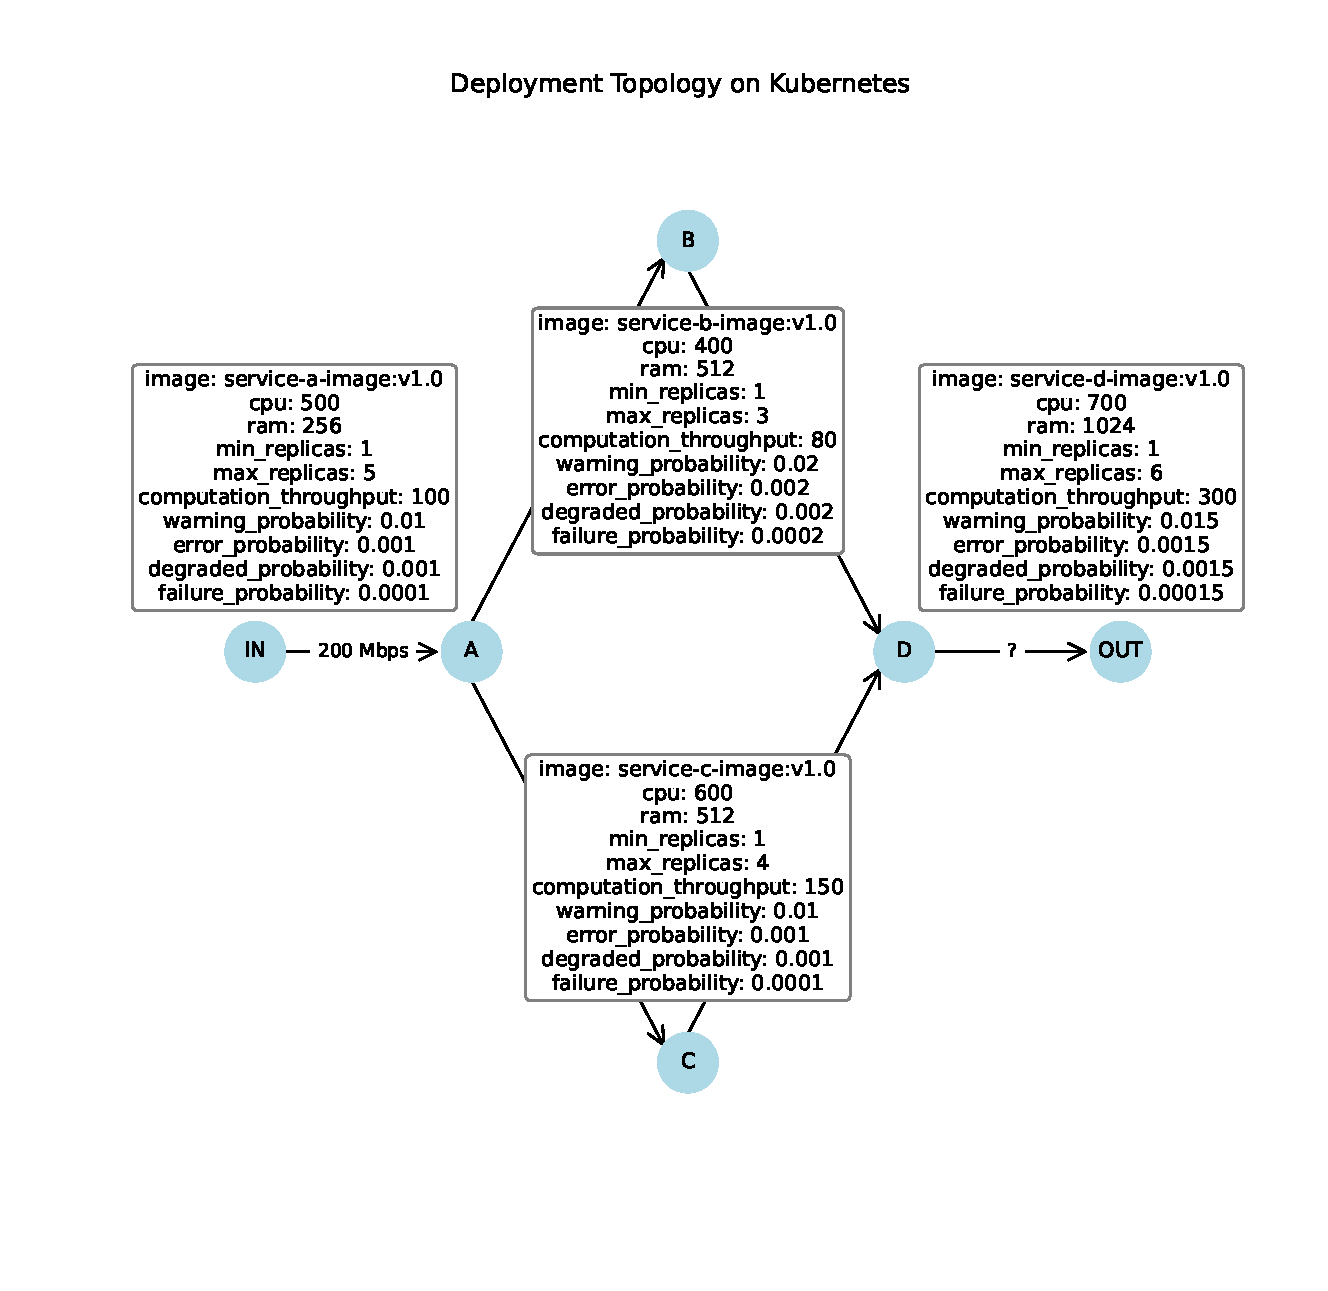
\includegraphics[trim=1.8cm 3.3cm 1.25cm 3.5cm, clip, width=0.5\textwidth]{figures/k8s_cluster_graph.pdf}
    \caption{A graph representation of a "Chained Services" cluster with four services}
    \label{fig:chained_services_graph}
\end{figure}

\subsubsection{Implementation of KARMA with CybMASDE}

% TODO:
% - Présenter le framework CybMASDE
% - Scénario normal, scénario DDoS (augmentation ponctuelle de volume données), scénario de défaillance (corruption ponctuelle des données), scénario de contention de ressources (priorisation), scénario mixte
% - Protocole d'expérimentation
%   - Baseline 1: Single-Agent w/o Soft Organizational Specifications
%   - Baseline 2: Single-Agent w/ Hard Organizational Specifications
%   - Baseline 3: Multi-Agent w/o Organizational Specifications
%   - Baseline 4: Multi-Agent w/ Organizational Specifications

\footnotetext[2]{\label{lnk:footnote_2}In our implementation by default $\alpha = 3$, $\sigma = 10$, $\kappa = 1$, and $ch = 1$}

The KARMA framework leverages \textit{Cyber Multi-Agent System Development Environment}~\textsuperscript{\autoref{lnk:footnote_1}} (CybMASDE) which is a general assisted-design MAS framework that seamlessly integrates into the KARMA framework~\textsuperscript{\autoref{lnk:footnote_2}}.
The framework includes:
\begin{enumerate}[label=\textbf{\arabic*)}, itemjoin={;\quad }]
    \item \textbf{Digital Twin Modeling:} A simulation environment replicates Kubernetes cluster using real-world traces
    \item \textbf{MARL Training:} \textit{MAPPO}~\cite{Yu2022} is used to train agents in the digital twin environment
    \item \textbf{Organizational Specifications:} Roles and missions defined for agents guide the training process, ensuring coordinated behavior and explainability
    \item \textbf{Deployment Integration:} Trained policies interact with the Kubernetes API to adjust pod replicas in real time.
\end{enumerate}

\subsubsection{Roles and Missions for Operational Resilience}

\noindent Following to the $\mathcal{M}OISE^+$~\cite{hubner2002moise} and the AICA architectural insights~\cite{kott2018autonomous}, we implemented four roles to address a specific degradation factor in a QoS.
% and defines the permissible actions of agents.
Each role is associated with a mission, containing a single sub-goal based on metrics.

\noindent \paragraph{\textbf{Bottleneck Manager}} 
%
The \textit{Bottleneck Manager} role is to monitor services for bottlenecks caused by imbalanced traffic flows. It is based on rules following these metrics:
\begin{enumerate}[label={}, itemjoin={;\quad }]
    \item \( T_{\text{in}}^i \): Incoming traffic for service \( i \) (Kbps)
    \item \( T_{\text{out}}^i \): Outgoing traffic for service \( i \)
    \item \( Q_{\text{pending}}^i \): Pending requests for service \( i \).
\end{enumerate}
A bottleneck is detected if: $Q_{\text{pending}}^i > Q_{\text{threshold}} \quad \text{or} \quad T_{\text{in}}^i > \alpha \cdot T_{\text{out}}^i$
where \( Q_{\text{threshold}} \) is the critical queue threshold, and \( \alpha > 1 \) is an amplification factor.

The associated mission aims to minimize the pending queue size to eliminate bottlenecks. The reward function is defined as: $R_{\text{bottleneck}} = - \sum_{i} Q_{\text{pending}}^i$
Agents are rewarded for reducing pending requests, optimizing the throughput~\cite{burns2016borg}.

\noindent \paragraph{\textbf{DDoS Manager}}

The \textit{DDoS Manager} role is to identify DDoS attacks by analyzing traffic anomalies:
\begin{enumerate}[label={}, itemjoin={;\quad }]
    \item \( R_{\text{rate}} \): Incoming request rate for the cluster.
    \item \( L_{\text{avg}} \): Average observed latency.
    \item \( \Delta T \): Change in traffic volume over a time window \( t \).
\end{enumerate}
A DDoS attack is detected when:
$R_{\text{rate}} > R_{\text{threshold}} \quad \text{and} \quad \Delta T > \Delta T_{\text{threshold}}$
where \( R_{\text{threshold}} \) is a critical traffic threshold.

The associated mission is to isolate affected services to minimize downtime with this reward function:
$R_{\text{ddos}} = - \left( \text{DownTime} \cdot w_{\text{d}} + L_{\text{avg}} \cdot w_{\text{l}} \right)$
where \( w_{\text{d}} \) and \( w_{\text{l}} \) are weights for downtime and latency, respectively~\cite{Liu2018}.

\noindent \paragraph{\textbf{Failure Manager}}

The \textit{Failure Manager} role is to monitor pod health and eliminates failed pods following this rule:
\begin{enumerate}[label={}, itemjoin={;\quad }]
    \item \( F_{\text{fail}}^i \): Number of failures for pod \( i \)
    \item \( S_{\text{status}}^i \): Status of pod \( i \) (e.g., \textit{CrashLoopBackOff}).
\end{enumerate}
A pod failure is detected if:
$F_{\text{fail}}^i > F_{\text{threshold}}$
where \( F_{\text{threshold}} \) is the maximum number of tolerated failures.

The associated mission minimizes downtime caused by repeated failures with this reward function:
$R_{\text{failure}} = - \sum_{i} T_{\text{downtime}}^i$
Agents are incentivized to quickly eliminate and restart failed services.

\noindent \paragraph{\textbf{Resource Manager}}

The \textit{Resource Manager} role is to prioritize critical services when resource contention occurs. The rules are based on:
\begin{enumerate}[label={}, itemjoin={;\quad }]
    \item \( U_{\text{cpu}}^i \): CPU utilization of service \( i \)
    \item \( U_{\text{mem}}^i \): Memory utilization of service \( i \)
    \item \( P_{\text{priority}}^i \): Priority level of service \( i \) (critical, normal, low).
\end{enumerate}
Contention is detected if total CPU usage exceeds a threshold:
$U_{\text{cpu}}^{\text{total}} > U_{\text{threshold}}$
Non-critical services are scaled down to free resources:
$\text{Replicas}_{\text{new}}^i = \max\left( \text{Replicas}_{\text{current}}^i - \delta, 1 \right)$

The associated mission ensures critical services by balancing resource usage with this reward function:
$R_{\text{resource}} = - \sum_{i \in \text{Critical}} \left( U_{\text{cpu}}^i + U_{\text{mem}}^i \right)$
Agents are rewarded for prioritizing services while maintaining efficient resource usage~\cite{shahrad2020resource}.

\

\subsubsection{Experimental Protocol}

\noindent To evaluate KARMA's performance in addressing the six gaps, we propose comparing baselines accross scenarios.

\paragraph{\textbf{Real-Cluster Integration \& Evaluation}}

KARMA couples simulation with real-cluster interaction by building a digital twin from real Kubernetes traces. Trained policies are deployed via the Kubernetes API, influencing the real cluster, while new traces refine the simulation. This ensures real-world applicability with agent training in a safe environment.

\paragraph{\textbf{Experimental Scenarios}}

\noindent Five experimental scenarios are defined to simulate key factors impacting operational resilience in Kubernetes:
%
\begin{enumerate}[label=\textbf{\arabic*)}, itemjoin={;\quad }]
    \item \textbf{Bottleneck Resolution:} Simulates scenarios where upstream services overload downstream services to maximize throughput by dynamically scaling replicas
    \item \textbf{DDoS Attack:} Models a sudden surge in traffic aimed at disrupting critical services to detect the attack, isolate affected services, and minimize downtime~\cite{Liu2018}
    \item \textbf{Pod Failures:} Pod crashes are triggered to evaluate the system's ability to restore affected services~\cite{burns2016borg}
    \item \textbf{Resource Contention:} Simulates high resource demand, requiring dynamic prioritization of critical services to maintain overall cluster functionality~\cite{Vhatkar2022}
    \item \textbf{Mixed Scenario:} Combines all scenarios to evaluate the system's adaptability and resilience.
\end{enumerate}

\paragraph{\textbf{Baselines from the literature}}
%
\noindent We selected three HPA systems as baselines:
\begin{enumerate}[label=\textbf{\arabic*)}, itemjoin={;\quad }]
    \item \textbf{AWARE:} An RL-based system that balances response time and throughput~\cite{aware2023}
    \item \textbf{Gym-HPA:} An RL environment for experimentation with various RL algorithms in simulation~\cite{gymhpa2022}
    \item \textbf{Rlad-core}~\cite{Rossi2019} A RL-based simulator which uses machine learning techniques to scale services, most notably Q-learning and Model-based algorithms.
\end{enumerate}

These baselines have been tested under the same five scenarios using source code when available.

\paragraph{\textbf{Baselines as ablation studies}}

\noindent To isolate the contributions of KARMA's components, ablation studies have been performed following these configurations:
%
\begin{itemize}
    \item \textbf{With/without MLP:} Evaluates the impact of using an MLP-based transitioner for digital-twin modeling.
    \item \textbf{With/without organizational specifications:} Tests hard and soft organizational constraints during training:
        \begin{itemize}
            \item \textit{Hard constraints:} Strictly enforce roles and missions.
            \item \textit{Soft constraints:} Allow exploratory actions with rewards based on organizational specifications.
        \end{itemize}
    \item \textbf{Multi-agent vs Mono-agent:} Compares a multi-agent configuration with a mono-agent baseline.
\end{itemize}

\paragraph{\textbf{Performance Metrics}}

\noindent For each scenario and baseline, the following metrics are collected:
%
\begin{enumerate}[label=\textbf{\arabic*)}, itemjoin={;\quad }]
    \item \textbf{Operational Resilience:} Based on the global reward from the success rate (\%), ratio of pending request (\%), average latency (ms)
    \item \textbf{Adversarial Robustness:} Based on the standard deviation of the reward and the recovery time after DDoS (s), percentage of services remaining available (\%)
    \item \textbf{Digital Twin Accuracy:} Based on the modeled transition model accuracy (\%), computed as the ratio of real cluster performance over the simulation's one
    \item \textbf{Automated MAS Generation:} Based on training convergence time (number of episodes)
    \item \textbf{Adaptability:} Based on the reward standard deviation variance over training episodes on all scenarios (\%)
    \item \textbf{Explainability:} Based on alignment of behaviors with roles/missions when given (\%), and qualitative evaluation of clustering of trajectories.
\end{enumerate}



\subsection{Results and Discussion}
\label{sec:results}

This section analyzes the performance of KARMA in addressing the six identified gaps.


\subsubsection{Gap 1: Operational Resilience}
Operational resilience evaluates the ability of the system to handle failures and maintain high QoS.
\begin{table}[h]
    \centering
    \caption{Operational resilience metrics across all scenarios.}
    \label{tab:operational_resilience}{\footnotesize
    \begin{tabular}{>{\raggedright\arraybackslash}m{2.7cm}>{\centering\arraybackslash}m{1.5cm}>{\centering\arraybackslash}m{1.5cm}>{\centering\arraybackslash}m{1.5cm}}
        \hline
        \textbf{Baseline} & \textbf{Success Rate (\%)} & \textbf{Latency Compliance (\%)} & \textbf{Pending Requests (\%)} \\
        \hline
        KHPA & 64.8 & 58.1 & 20.7 \\
        Gym-HPA & 73.1 & 65.7 & 20.8 \\
        Rlad-core & 77.4 & 70.1 & 15.9 \\
        AWARE & 80.6 & 73.8 & 13.3 \\
        Single-Agent w/o Org. Spec. & 72.6 & 65.4 & 17.0 \\
        Single-Agent w/ Hard Org. Spec. & 80.8 & 72.5 & 15.4 \\
        Multi-Agent w/o Org. Spec. & 87.7 & 81.5 & 9.3 \\
        Multi-Agent w/ Soft Org. Spec. & 82.0 & 74.7 & 15.0 \\
        \textbf{Multi-Agent w/ Hard Org. Spec. (KARMA)} & \textbf{90.9} & \textbf{85.7} & \textbf{5.9} \\
        \hline
    \end{tabular}}
\end{table}

\autoref{tab:operational_resilience} presents a comparison of KARMA against existing baselines. The results show that KARMA achieves the highest success rate (\textbf{90.9\%}), surpassing all baselines including AWARE (80.6\%) and Rlad-core (\textbf{77.4\%}). Similarly, the latency compliance of KARMA is the highest at \textbf{85.7\%}, while the lowest pending requests ratio (\textbf{5.9\%}) suggests efficient handling of workload variations.

KARMA's performance stems from its structured multi-agent coordination, which optimally distributes resources based on failure contexts, avoiding redundant or conflicting scaling actions—issues common in single-agent RL-based autoscalers.
%
Reactive, threshold-based autoscalers like KHPA and Gym-HPA struggle with dynamic workloads, leading to higher pending requests and lower success rates. AWARE and Rlad-core improve response time and throughput but lack multi-agent coordination, resulting in slower reactions in adversarial scenarios. Single-Agent w/o Organizational Specifications suffers from inefficient resource allocation, while Single-Agent w/ Hard Organizational Specifications benefits from structured decision-making but still lacks distributed coordination.

KARMA's role-based coordination minimizes inefficiencies and enhances decision stability. Its hierarchical decomposition of objectives enables independent yet complementary decisions, leading to more resilient autoscaling.

The results also underscore the value of organizational constraints. Multi-agent systems with soft constraints (82.0\% success rate) outperform single-agent approaches, but KARMA's hard constraints achieve the best results, eliminating conflicting agent behaviors and optimizing scaling.



\subsubsection{Gap 2: Adversarial Conditions}

Adversarial conditions evaluate the system's robustness against disruptive scenarios such as DDoS attacks.
\begin{table}[h]
    \centering
    \caption{Performance under adversarial conditions (DDoS scenario).}
    \label{tab:adversarial_conditions}{
        \footnotesize
    \begin{tabular}{>{\raggedright\arraybackslash}m{3.6cm}>{\centering\arraybackslash}m{1.8cm}>{\centering\arraybackslash}m{2cm}}
        \hline
        \textbf{Baseline} & \textbf{Recovery Time (s)} & \textbf{Service Availability (\%)} \\
        \hline
        KHPA & 80.7 & 65.6 \\
        Gym-HPA & 66.2 & 72.6 \\
        Rlad-core & 37.4 & 78.3 \\
        AWARE & 49.5 & 83.6 \\
        Single-Agent w/o Org. Spec. & 60.3 & 72.4 \\
        Single-Agent w/ Hard Org. Spec. & 48.5 & 77.5 \\
        Multi-Agent w/o Org. Spec. & 43.5 & 82.0 \\
        Multi-Agent w/ Soft Org. Spec. & 38.8 & 86.0 \\
        \textbf{Multi-Agent w/ Hard Org. Spec. (KARMA)} & \textbf{33.0} & \textbf{90.7} \\
        \hline
    \end{tabular}}
\end{table}

\autoref{tab:adversarial_conditions} compares recovery times and service availability in the \textit{DDoS Attack} scenario. KARMA achieves the fastest recovery time (\textbf{33.0s}), outperforming AWARE (\textbf{38.8s}) and Rlad-core (\textbf{43.5s}). It also ensures a good service availability at \textbf{90.7\%}, reducing downtime compared to AWARE (\textbf{83.6\%}).

Traditional autoscalers like KHPA and Gym-HPA rely on reactive threshold-based scaling, leading to slower recovery and lower service availability under attacks. RL-based methods such as Rlad-core and AWARE improve resilience but lack structured coordination, making them less effective against adversarial spikes. Single-agent approaches struggle with balancing attack mitigation and resource optimization, while multi-agent models with soft constraints allow exploratory actions that sometimes delay optimal responses.

KARMA's proactive adversarial learning and structured coordination enable it to anticipate attacks rather than react after degradation. Explicit role-based constraints ensure agents prioritize critical scaling actions, resulting in faster mitigation and higher availability. These results highlight the effectiveness of multi-agent structured learning in security-sensitive autoscaling, where traditional methods exhibit slower adaptation and prolonged downtime.


\subsubsection{Gap 3: Digital Twin Modeling}

The accuracy of the digital twin model is critical for training agents under realistic conditions.
\begin{table}[h]
    \centering
    \caption{Transition models accuracy across all scenarios.}
    \label{tab:digital_twin_accuracy}{
        \footnotesize
    \begin{tabular}{>{\raggedright\arraybackslash}m{6cm}>{\centering\arraybackslash}m{2cm}}
        \hline
        \textbf{Baseline} & \textbf{Accuracy (\%)} \\
        \hline
        Without MLP Transition Model & 83.5 \\
        \textbf{With MLP Transition Model (KARMA)} & \textbf{94.9} \\
        \hline
    \end{tabular}}
\end{table}

\autoref{tab:digital_twin_accuracy} compares the accuracy of different digital twin models. The results show that KARMA achieves \textbf{94.9\%} accuracy, outperforming the non-MLP model (\textbf{83.5\%}), which struggles to generalize across varying workloads.

The improvement stems from the MLP model's ability to capture non-linear dependencies between workload fluctuations, resource allocation, and scaling actions. Without this feature, the system fails to model complex cluster behaviors accurately.
%
By leveraging a neural network for transition modeling, KARMA ensures a more reliable digital twin, allowing agents to train under near-realistic conditions. This reduces the risk of poor decision-making when policies transfer to production, reinforcing the importance of high-fidelity simulations.



\subsubsection{Gap 4: Automated MAS Generation}

The efficiency of generating a MAS is evaluated in terms of convergence time and training overhead. \autoref{tab:mas_generation_efficiency} presents the results across concerned scenarios while \autoref{fig:learning_curves} shows learning curves in the mixed scenario over 2000 episodes.

\begin{table}[h]
    \centering
    \caption{MAS generation efficiency across all scenarios.}
    \label{tab:mas_generation_efficiency}{
        \footnotesize
    \begin{tabular}{>{\raggedright\arraybackslash}m{3.5cm}>{\centering\arraybackslash}m{2cm}>{\centering\arraybackslash}m{2cm}}
        \hline
        \textbf{Baseline} & \textbf{Convergence Time (episodes)} & \textbf{Training Overhead (hours)} \\
        \hline
        Multi-Agent w/o Org. Spec. & 1800 & 4 \\
        \textbf{Multi-Agent w/ Hard Org. Spec. (KARMA)} & \textbf{950} & \textbf{1.5} \\
        \hline
    \end{tabular}}
\end{table}

The role-guided learning narrows the search space for optimal policies, enabling faster convergence and reduced computational costs. These efficiency gains are particularly important for scaling MAS solutions to complex environments.

The learning curves in \autoref{fig:learning_curves} demonstrate that KARMA achieves stable convergence significantly faster than the baseline without organizational specifications. By episode 950, KARMA exhibits minimal variance in cumulative rewards, whereas the baseline requires nearly double the episodes (1800) to reach comparable performance. This highlights the role of organizational constraints in guiding agents toward effective policies, thereby reducing exploration overhead.

\autoref{tab:mas_generation_efficiency}, shows reduced \textit{Convergence Time} by approximately \textbf{47\%} compared to Multi-Agent w/o Org. Spec., showcasing the efficiency of role-guided learning in minimizing unnecessary exploration. Moreover, \textit{Training Overhead} is reduced by \textbf{62.5\%}, showing a better practicality for large-scale systems where computational resources are a limiting factor.

\begin{figure}[h!]
    \centering
    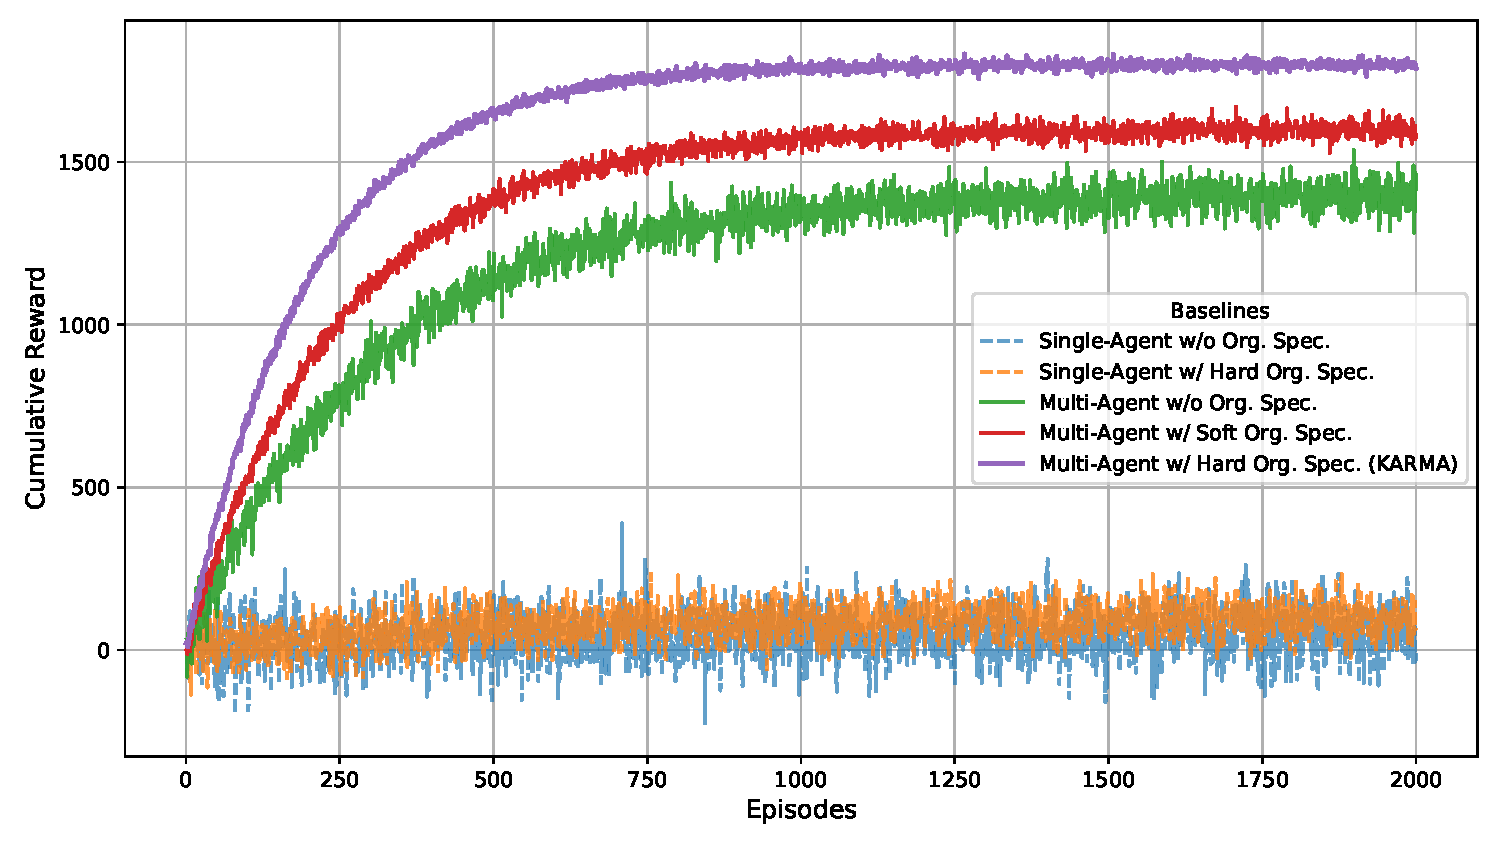
\includegraphics[width=0.49\textwidth]{figures/learning_curves.pdf}
    \caption{Learning curves across baselines for the mixed scenario over 2000 episodes.}
    \label{fig:learning_curves}
\end{figure}


\subsubsection{Gap 5: Adaptability}

Adaptability assesses the ability of the system to maintain performance under dynamic workloads accross scenarios.
\begin{table}[h]
    \centering
    \caption{Comparison of adaptability metrics in the mixed scenario.}
    \label{tab:adaptability_comparison}{
    \footnotesize
    \begin{tabular}{>{\raggedright\arraybackslash}m{5cm}>{\centering\arraybackslash}m{3cm}}
        \hline
        \textbf{Baseline} & \textbf{Reward s.t.d (\%)} \\
        \hline
        Single-Agent w/o Org. Spec. & 11.1 \\
        Single-Agent w/ Hard Org. Spec. & 11.1 \\
        Multi-Agent w/o Org. Spec. & 10.7 \\
        Multi-Agent w/ Soft Org. Spec. & 9.0 \\
        \textbf{Multi-Agent w/ Hard Org. Spec. (KARMA)} & \textbf{5.3} \\
        \hline
    \end{tabular}}
\end{table}

\autoref{tab:adaptability_comparison} shows that KARMA achieves the lowest reward standard deviation (\textbf{5.3\%}), indicating a highly stable performance, outperforming Multi-Agent w/ Soft Org. Spec. (\textbf{9.0\%}) and Multi-Agent w/o Org. Spec. (\textbf{10.7\%}).

In the \textit{Mixed Scenario}, single-agent models exhibit higher variance as they must balance multiple competing objectives without specialization. Multi-agent approaches improve adaptability, but without structured coordination, fluctuations remain. The use of soft organizational constraints stabilizes performance, though some exploratory variations persist.

KARMA's hierarchical reinforcement learning ensures lower variability by decomposing the overarching goal into specialized sub-goals. This structured approach enables agents to focus on well-defined objectives, reducing conflicting decisions and improving overall stability.
%
These findings underscore the importance of structured learning frameworks in autoscaling. By enforcing clear agent specializations, KARMA enhances adaptability, ensuring resilient performance across unpredictable workload conditions.


\subsubsection{Gap 6: Explainability}
\label{subsec:gap_explainability}

Explainability is qualitatively evaluated through trajectory clustering and quantitatively through the alignment of agent behaviors with predefined roles and missions.
\noindent \autoref{fig:trajectory_clustering_hrl} illustrates the dendrogram generated by hierarchical clustering of agents' action sequences with the four roles applied, using DTW as the similarity measure. The figure highlights the emergence of four distinct clusters, each corresponding to a specific organizational role, demonstrating the ability of the agents' behaviors to align with the predefined roles.

\begin{figure}[h!]
    \centering
    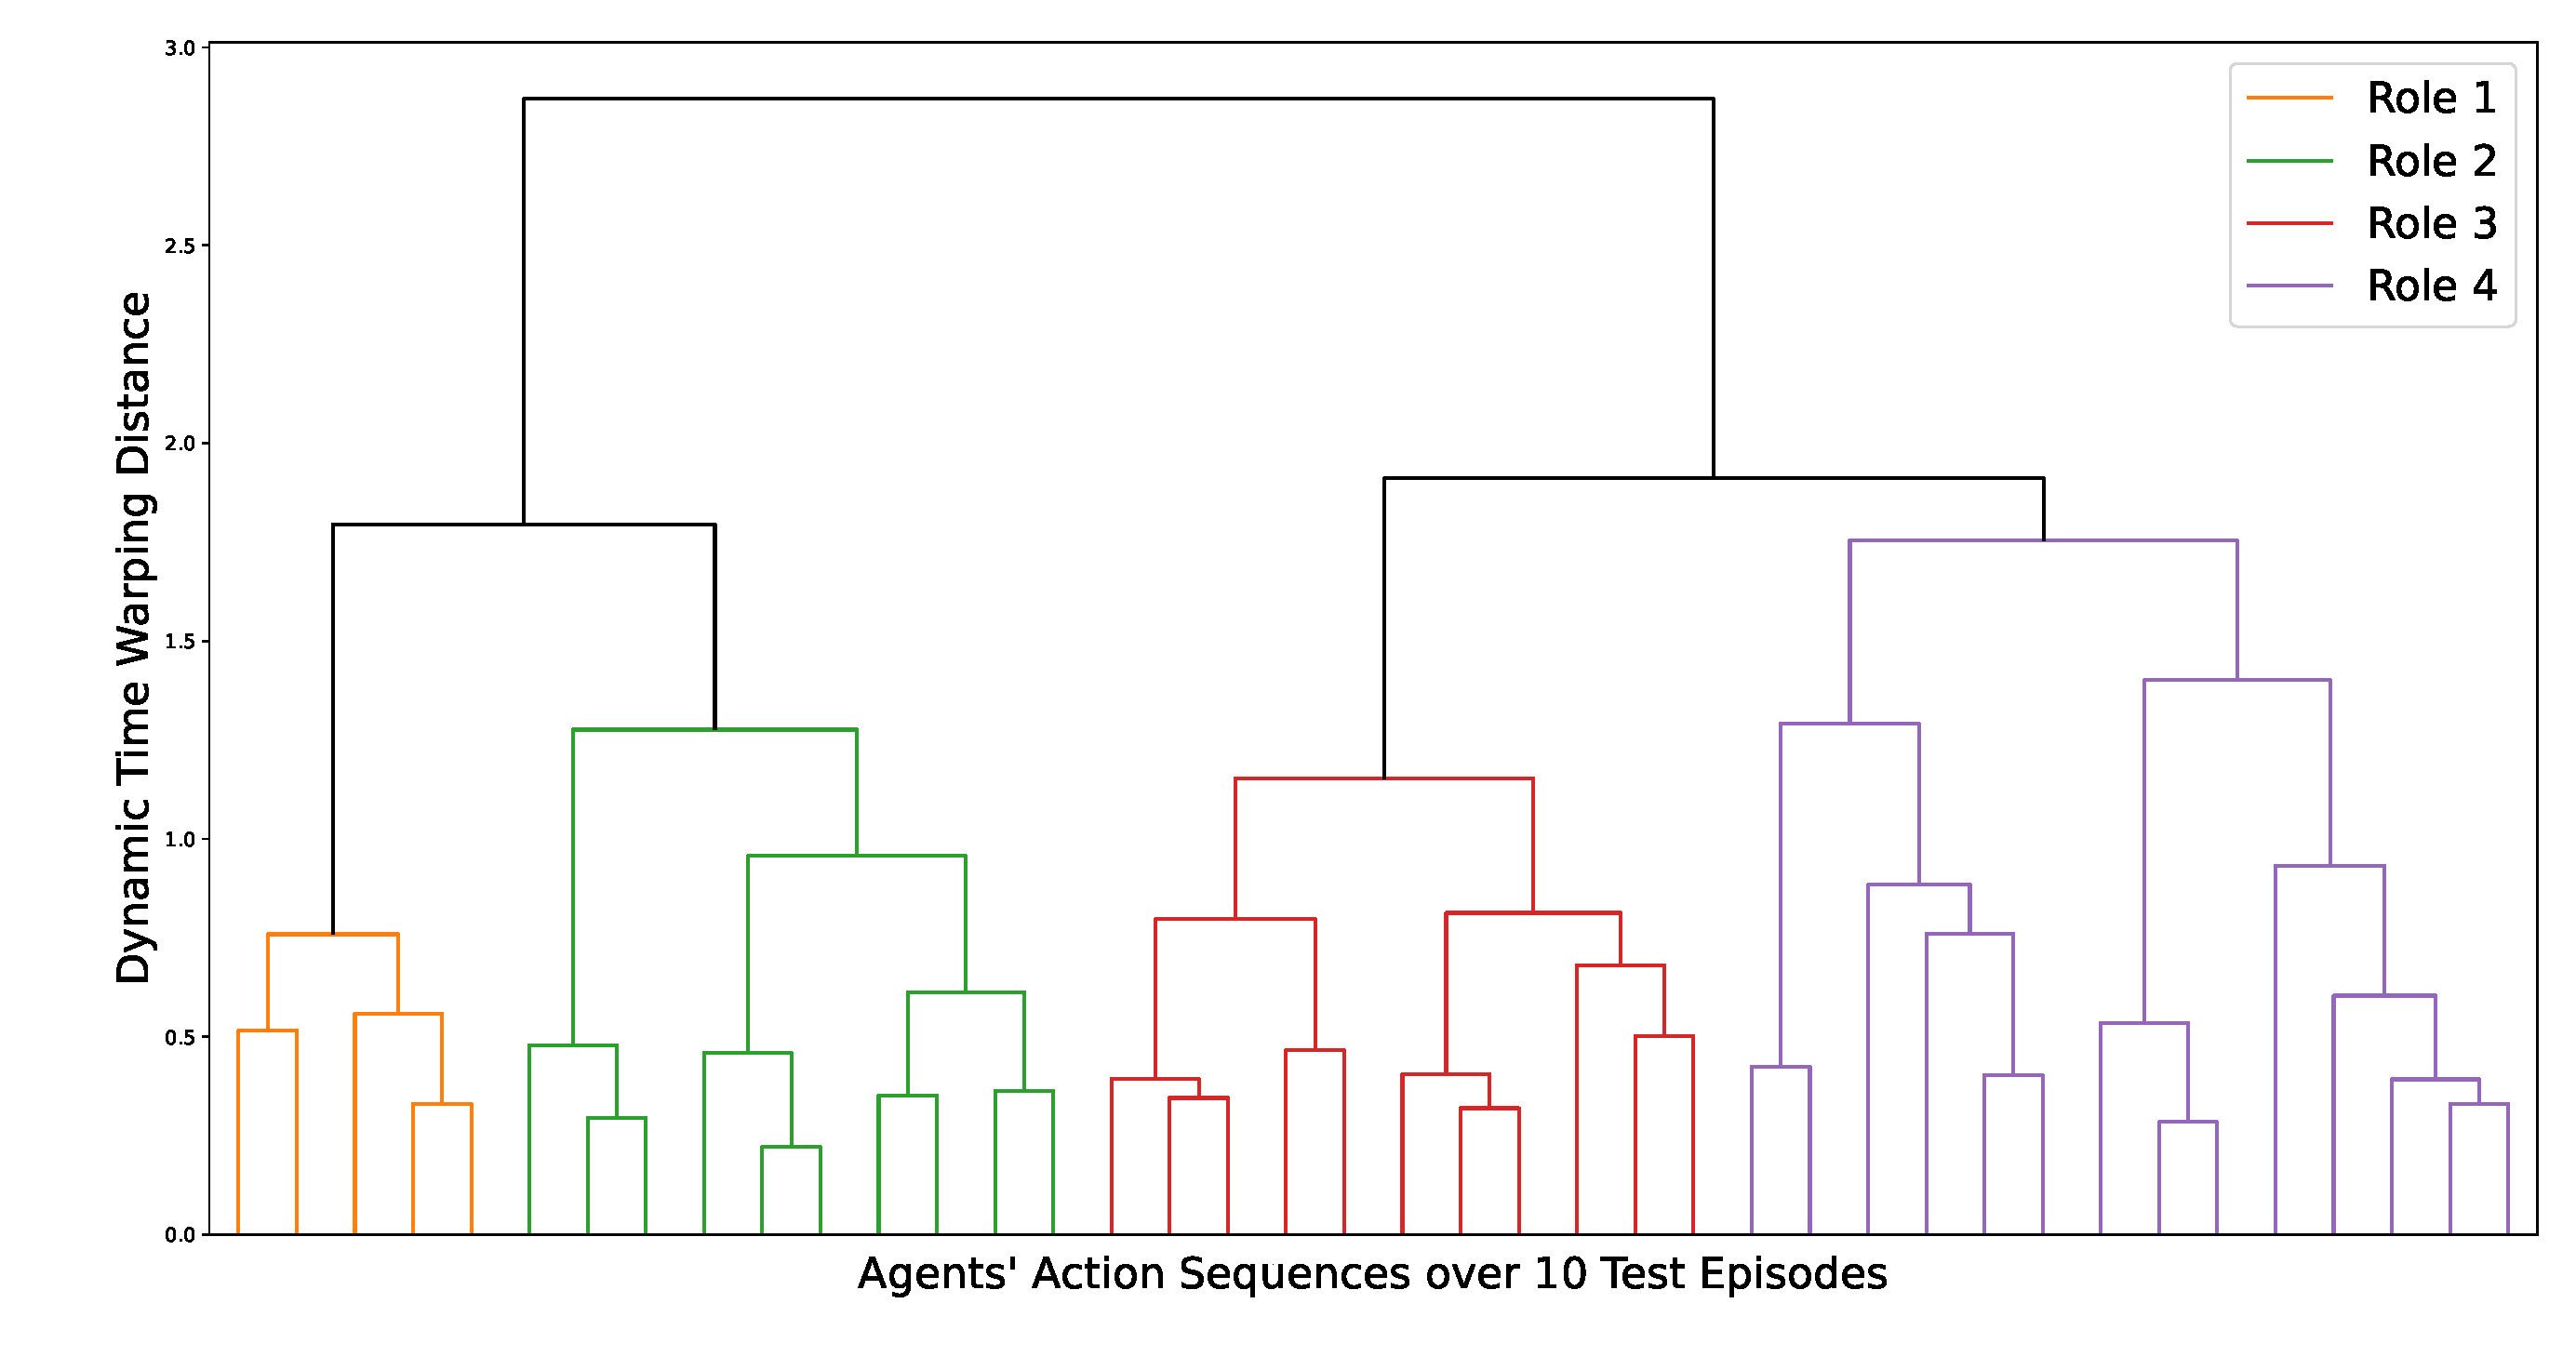
\includegraphics[width=0.49\textwidth]{figures/role_hierarchical_clustering.pdf}
    \caption{Dendrogram obtained after hierarchical clustering of agent trajectories for role inference in the mixed scenario.}
    \label{fig:trajectory_clustering_hrl}
\end{figure}

\begin{table}[h!]
    \centering
    \caption{Alignment of Agent Behavior with Roles and Missions.}
    \label{tab:alignment}
    {\footnotesize
    \begin{tabular}{>{\raggedright\arraybackslash}m{4.1cm}>{\centering\arraybackslash}m{1.5cm}>
    {\centering\arraybackslash}m{1.5cm}}
    \toprule
    \textbf{Baseline} & \textbf{Alignment Score (\%)} & \textbf{Clustering Purity (\%)} \\
    \midrule
    Multi-Agent w/o Org. Spec. & $\emptyset$ & 62.7 \\
    Multi-Agent w/ Soft Org. Spec. & 85.3 & 70.1 \\
    \textbf{Multi-Agent w/ Hard Org. Spec. (KARMA)} & \textbf{96.2} & \textbf{89.4} \\
    \bottomrule
    \end{tabular}
    }
\end{table}

KARMA shows the emergence of distinct behavioral patterns aligned with predefined roles validates KARMA's organizational model and has the highest alignment score (\textbf{96.2\%}), significantly outperforming Multi-Agent w/o Org. Spec. (\textbf{85.3\%}), showcasing well-coordinated agent behaviors. In adversarial scenarios, clustering purity is highest for KARMA, reflecting the clear differentiation of agent behaviors under organizational constraints.
%
Distinct clusters validate the role-specific behaviors and highlight the interpretability of agents. Baselines without organizational specifications show reduced explainability, as evidenced by lower clustering purity and alignment scores with soft organizational constraints.

% \subsubsection{General discussion}

% The experimental results demonstrate that KARMA effectively addresses several critical gaps in Kubernetes autoscaling. By integrating MARL with organizational principles, KARMA achieves notable improvements in operational resilience, adversarial robustness, and explainability. Its ability to decompose complex goals into roles and missions ensures coordinated agent behavior, as reflected in the high success rates, reduced recovery times, and alignment with predefined roles observed across all scenarios. The use of a digital twin environment, enhanced by an MLP-based transition model, further strengthens KARMA's capacity to simulate realistic conditions, facilitating robust training and better policy generalization.

% However, KARMA is not without limitations. While it shows advancements in adaptability, its dependence on domain expertise for defining roles and missions could limit its applicability in domains where such expertise is scarce. Additionally, the computational overhead required for multi-agent training and digital twin modeling remains a challenge for large-scale deployments. The results also indicate that while KARMA effectively reduces latency and pending requests, some baselines, such as Rlad-core, perform comparably in specific scenarios like resource contention, highlighting areas where further refinement may be needed.

\subsection{Conclusion}
\label{sec:conclusion}
% Conclusion
%  - Résumé
%  - Résumé des Points faibles et Perspectives

This paper presented KARMA, a framework aimed at improving the operational resilience of Kubernetes clusters through a MAS-based approach.
The experimental results demonstrate that KARMA effectively addresses several critical gaps in Kubernetes autoscaling. By integrating MARL with organizational principles, KARMA achieves improvements in adversarial robustness, and explainability. Its ability to decompose complex goals into roles and missions ensures coordinated agent behavior, as reflected in the high success rates, reduced recovery times. The use of MLP-based transition model, further strengthens KARMA's capacity to simulate realistic conditions, facilitating better policy generalization.
%
% The main contributions of this work include:
% \begin{itemize}
%     \item \textbf{Digital Twin Environment:} A realistic and representative simulation model derived from cluster traces, enabling safe and efficient policy learning through a digital twin.
%     \item \textbf{Organizationally Guided Design:} The use of roles and missions to decompose operational resilience into manageable sub-goals, providing a systematic method for agent coordination and decision-making.
%     \item \textbf{Multi-Agent Reinforcement Learning (MARL):} Leveraging MARL algorithms to train agents collaboratively, ensuring adaptability and robustness in complex, multi-goal scenarios.
%     \item \textbf{Explainability and Analysis:} Analyzing agent behaviors using trajectory clustering and inter-agent interaction detection, enhancing interpretability and trust in agent decisions.
%     \item \textbf{Adversarial Scenario Handling:} Demonstrating the resilience of the proposed framework in scenarios such as DDoS attacks, which are critical for the reliability of cloud-native systems.
% \end{itemize}
%
% \

However, some aspects need to be further explored:
\begin{enumerate}[label=\textbf{\arabic*)}, itemjoin={;\quad }]
    \item \textbf{Simulation-to-Reality Gap:} Even though we generate a near-realistic simulation model from environment traces, we still need to better simulate unaccounted API latencies and unexpected system failures
    \item \textbf{Dependence on Domain Expertise:} Defining roles, missions, and reward structures relies heavily on domain-specific knowledge, which may limit the framework's generalizability to other scenarios
    \item \textbf{Computational Overhead:} The training process with multi-agent configurations and organizational constraints requires substantial computational resources, posing challenges for real clusters.
    % \item \textbf{Sensitivity to Workload Shifts:} While KARMA demonstrates adaptability, abrupt changes in workload patterns or cluster configurations may require retraining or fine-tuning of agent policies.
    % \item \textbf{Evaluation Scope:} Although the framework was tested under diverse scenarios, including adversarial conditions, its performance on larger and more heterogeneous clusters remains to be validated.
\end{enumerate}

Building on these initial results, we plan to explore:
\begin{enumerate}[label=\textbf{\arabic*)}, itemjoin={;\quad }]
    \item \textbf{Automated Role and Mission Generation:} Improving non-supervised learning methods or pre-trained knowledge bases to automatically define roles and missions (Meta-learning), reducing the reliance on domain expertise
    % \item \textbf{Efficient Training Pipelines:} Exploring optimization techniques, such as transfer learning or distributed training, to mitigate the computational overhead of multi-agent training.
    \item \textbf{Dynamic Role Adjustment:} Investigating mechanisms for agents to dynamically adapt their roles and missions, enhancing flexibility and responsiveness
    \item \textbf{Generalization to Larger Clusters:} Extending the framework to more complex, large-scale Kubernetes deployments with heterogeneous configurations.
    % \item \textbf{Integration with Real-Time Monitoring:} Incorporating advanced monitoring systems to further refine the digital twin model and provide more accurate state representations.
\end{enumerate}

% While KARMA is not a universal solution to all Kubernetes autoscaling challenges, it provides a step forward in addressing key gaps in operational resilience, adaptability, and explainability. The framework's combination of MARL and organizational principles offers a promising foundation for future research and development.


\section{Résultats et discussion}
\begin{itemize}

    \item Montrer comment nous utilisons CybSMADE pour résoudre le problème
          \begin{itemize}
              \item En utilisant également le modèle AICA
          \end{itemize}
\end{itemize}

\section{Tendances générales qui ressortent des résultats et de la synthèse}
\begin{itemize}
    \item Discuter le niveau de l'impact de la méthode
          \begin{itemize}
              \item Sans spécifications initiales
              \item Avec spécifications initiales (incluant l'AICA)
          \end{itemize}
    \item Discuter des organisations qui semblent pertinentes avec une analyse quantitative sur les 3 cas d'étude
    \item Discuter des résultats et la cohérence de ces-derniers par rapport à d'autres résultats
\end{itemize}
%************************************************
\chapter{Conclusion et travaux futurs}\label{ch:conclusion} % $\mathbb{ZNR}$
%************************************************

\begin{itemize}
    \item Conclusion sur la partie "académique" de la contribution
    \item Expliquer qu'au-delà de répondre à la question de la thèse, la contribution permet aussi de répondre à des problèmes de l'industrie sur la protection de système sur certains aspects
\end{itemize}

\section{Vers une application industrielle pour la prise de décision en matière de Cyberdéfense}
\begin{itemize}
    \item Simuler des événements qui pourraient arriver et essayer de gagner de l'expérience en prévision du moment où l'attaque sera déjà en cours
    \item Parler de l'expérience de l'approche / outil en industrie avec Thales
\end{itemize}

\section{Limitations et perspectives}
\begin{itemize}
    \item Evoquer la difficulté du passage à l'échelle
    \item Le manque de maturité (TRL ne dépasse pas 3/4)
    \item Travaux connexes sur l'explicabilité au niveau collectif via d'autres approches pas nécéssairement dans la sécurité des réseaux...
\end{itemize}


%********************************************************************
% Other Stuff in the Back
%*******************************************************
\cleardoublepage%********************************************************************
% Bibliography
%*******************************************************
% work-around to have small caps also here in the headline
\manualmark
\markboth{\spacedlowsmallcaps{\bibname}}{\spacedlowsmallcaps{\bibname}} % work-around to have small caps also
%\phantomsection 
\refstepcounter{dummy}
\addtocontents{toc}{\protect\vspace{\beforebibskip}} % to have the bib a bit from the rest in the toc
\addcontentsline{toc}{part}{\tocEntry{\bibname}}
\label{app:bibliography}
\printbibliography

% \cleardoublepage%*******************************************************
% Declaration
%*******************************************************
\refstepcounter{dummy}
\pdfbookmark[0]{Declaration}{declaration}
\chapter*{Declaration}
\thispagestyle{empty}
Put your declaration here.
\bigskip
 
\noindent\textit{\myLocation, \myTime}

\smallskip

\begin{flushright}
    \begin{tabular}{m{5cm}}
        \\ \hline
        \centering\myName \\
    \end{tabular}
\end{flushright}

% \cleardoublepage\pagestyle{empty}

\hfill

\vfill


\pdfbookmark[0]{Colophon}{colophon}
\section*{Colophon}
This document was typeset using the typographical look-and-feel \texttt{classicthesis} developed by Andr\'e Miede. 
The style was inspired by Robert Bringhurst's seminal book on typography ``\emph{The Elements of Typographic Style}''. 
\texttt{classicthesis} is available for both \LaTeX\ and \mLyX: 
\begin{center}
\url{https://bitbucket.org/amiede/classicthesis/}
\end{center}
Happy users of \texttt{classicthesis} usually send a real postcard to the author, a collection of postcards received so far is featured here: 
\begin{center}
\url{http://postcards.miede.de/}
\end{center}
 
\bigskip

\noindent\finalVersionString

%Hermann Zapf's \emph{Palatino} and \emph{Euler} type faces (Type~1 PostScript fonts \emph{URW
%Palladio L} and \emph{FPL}) are used. The ``typewriter'' text is typeset in \emph{Bera Mono}, 
%originally developed by Bitstream, Inc. as ``Bitstream Vera''. (Type~1 PostScript fonts were made 
%available by Malte Rosenau and
%Ulrich Dirr.)

%\paragraph{note:} The custom size of the textblock was calculated
%using the directions given by Mr. Bringhurst (pages 26--29 and
%175/176). 10~pt Palatino needs  133.21~pt for the string
%``abcdefghijklmnopqrstuvwxyz''. This yields a good line length between
%24--26~pc (288--312~pt). Using a ``\emph{double square textblock}''
%with a 1:2 ratio this results in a textblock of 312:624~pt (which
%includes the headline in this design). A good alternative would be the
%``\emph{golden section textblock}'' with a ratio of 1:1.62, here
%312:505.44~pt. For comparison, \texttt{DIV9} of the \texttt{typearea}
%package results in a line length of 389~pt (32.4~pc), which is by far
%too long. However, this information will only be of interest for
%hardcore pseudo-typographers like me.%
%
%To make your own calculations, use the following commands and look up
%the corresponding lengths in the book:
%\begin{verbatim}
%    \settowidth{\abcd}{abcdefghijklmnopqrstuvwxyz}
%    \the\abcd\ % prints the value of the length
%\end{verbatim}
%Please see the file \texttt{classicthesis.sty} for some precalculated 
%values for Palatino and Minion.
%
%    \settowidth{\abcd}{abcdefghijklmnopqrstuvwxyz}
%    \the\abcd\ % prints the value of the length






% ********************************************************************
% Backmatter
%*******************************************************
\appendix
%\renewcommand{\thechapter}{\alph{chapter}}
\cleardoublepage
% \part{Appendix}
%********************************************************************
% Appendix
%*******************************************************
% If problems with the headers: get headings in appendix etc. right
%\markboth{\spacedlowsmallcaps{Appendix}}{\spacedlowsmallcaps{Appendix}}
\part{Appendices}

\chapter{List of included papers}

\chapter{Experiments details}


\end{document}
% ********************************************************************
